\documentclass[14pt,a4paper]{report}
\usepackage[english]{babel}
\usepackage[utf8]{inputenc}
\usepackage{fancyhdr}
\usepackage{indentfirst}
\usepackage{graphicx}
\usepackage{newlfont}
%\usepackage{natbib}
\usepackage{geometry}
\usepackage{makeidx}
\usepackage{url}
\usepackage{subfig}
\usepackage{float}


%\usepackage{natbib}
\geometry{a4paper,tmargin=2.5cm,bmargin=3cm,lmargin=3.5cm,rmargin=2.5cm}

\hyphenation{sil-la-ba-zio-ne pa-ren-te-si}

\pagestyle{fancy}\addtolength{\headwidth}{20pt}
\chead{}
\renewcommand{\sfdefault}{phv}
\renewcommand{\familydefault}{\sfdefault}
\linespread{1.5}


\usepackage{afterpage}

\newcommand\blankpage{%
    \null%
    \thispagestyle{empty}%
    \addtocounter{page}{-1}%
    \newpage}
  
\begin{document}

\chead{Tesi di Laurea --- Anno Accademico 2016 --- 2017}

%%%%%%%%%%%%%%%%%%FRONT

%modificare questo file inserendo i propri dati
%\begin{titlepage}
% !TEX root = Tesi.tex


\thispagestyle{empty}
\begin{center}

        
\includegraphics[width=3cm]{images/logo}\\
\vspace{1cm}
       {\Huge UNIVERSIT\`A DEGLI STUDI}\\
        \vspace{8mm}                                                  %vspace = per spaziare le righe
        {\Huge DELL' AQUILA}\\
        \vspace{1.3cm}
        \vspace{2.2cm}

         {\Large TESI DI LAUREA} \\

        \vspace{8mm}
        {\LARGE \bfseries ``Enhancing e-Commerce applications through web data mining and real usage data``} \\
        \vspace{2.8cm}
        {\large Corso di Laurea Specialistica}\\
        \vspace{18mm}
    \end{center}
\vspace{20mm}
   \begin{tabular}{l}
        { Candidato:}\\
        { \textit{Fabio Righi}}\\
      \end{tabular}
    \hfill
    \begin{tabular}{l}
        { Relatore:}\\
        { \textit{Dott.  Romina Eramo}}\\
    \end{tabular}
%In caso di presenza di co.relatore togliere i commenti
% \begin{tabular}{l}
%{ Correlatore:}\\
%{ Prof.  Nome Cognome}\\
 %   \end{tabular}
%\end{titlepage}
\vspace{20mm}
\begin{center}
{\large Anno Accademico 2015/2016}
\end{center}

\afterpage{\blankpage}

%%%%%%%%%%%%%%%%%%%%%%%%%% ABSTRACT

\chapter*{\LARGE Abstract}
\thispagestyle{empty}
\renewcommand{\sfdefault}{phv}
Marketing personalisation is becoming a key focus area in communication studies and development, and will draw more and more attention of marketers in the next few years. For being able to effectively personalise the experiences of their customers, brands must overcome challenges that range from learning customer behaviour as they interact with the brand itself, to creating customer experiences that are tailored according to brand knowledge of individual preferences.

If in the past brands had not enough data to understand their customers at a personal level, nowadays things are moving towards an entirely different scenario, in which big data plays a fundamental role. For the first time, companies are able to distinguish customers beyond the mere demographic dimensions, leveraging the information collected in both the virtual and the physical worlds, and detecting  and analysing patterns in their behaviour.

In this work, we describe how marketing personalisation can be achieved by coupling  the customer information resulting from web data mining with the device tracking allowed by the Internet of Things. We will apply Model Driven Engineering techniques to classify and analyse the gathered data and, from that, to deliver unique and more effective online interactions between a brand and its consumers.


%%%%%%%%%%%%%%%%%%%%%%%%%%%ACKNOWLEDGEMENTS

\chapter*{\LARGE Acknowledgements}
\thispagestyle{empty}
\renewcommand{\sfdefault}{phv}
Lorem ipsum dolor sit amet, consectetur adipisici elit, sed eiusmod tempor incidunt ut labore et dolore magna aliqua.
Ut enim ad minim veniam, quis nostrud exercitation ullamco laboris nisi ut aliquid ex ea commodi consequat. Quis aute iure reprehenderit in voluptate velit esse cillum dolore eu fugiat nulla pariatur. Excepteur sint obcaecat cupiditat non proident, sunt in culpa qui officia deserunt mollit anim id est laborum



%%%%%%%%%%%%%%%%%INDEX
\tableofcontents

%%%%%%%%%%%%%%%%%%%%%%CHAPTERS

% !TEX root = Tesi.tex
\chapter*{Introduction}

To learn and discover user preferences by analysing actual interactions and to cleverly take advantage of that learning: How can that be achieved? In the first chapter of this thesis, we answer this question by introducing the reader to two possible sources of real usage data: the Internet of Things and the Web Mining process. In addition, we present the software development techniques used for modeling the data gathered from those sources.

Following that general introduction, we proceed to Chapter 2, in which we examine the current state-of-the art of those information sources as well as their related pattern-recognition techniques.

In Chapter 3, we discuss an approach that blends together the discussed data acquisition channels. We also offer different use-case scenarios in which an actual eCommerce platform dialogues with a physical retail store for creating a singular brand experience.

Starting from Chapter 4, we begin to model the data presented previously by using Model Driven Engineering notions and by describing metamodels and models for the domain and the data occurrences. 

We proceed then with Chapter 5, illustrating a possible model transformation for the eCommerce platform based on the real usage dynamic instance, to offer users a more customised experience.

After the modeling and processing phase, we continue with discussing a case study. Chapter 6 introduces the eCommerce Magento platform, and suggests a possible transformed model serialisation that would result in compatible code within the Magento ecosystem.

The last chapter covers related works, conclusions and a possible evolution for the presented approach.

\addcontentsline{toc}{chapter}{Introduction}



 % !TEX root = Tesi.tex
\chead{}
\chapter{Background}

\section{The Internet of Things and the Web}
  
During the last few years, and in an increasing manner, we have been standing at the forefront of a world where virtually everything can be connected directly to the Internet. This has resulted in an increasingly connected world where emerging technologies enable objects to be linked among themselves through the use of new devices and sensors.

This new era of the Internet has become visible in our everyday lives: from souped-up gadgets tracking our every move to environments capable of predicting our actions and emotions, the list keeps growing every day.

The Internet, consisting of things, rather than just computers, is becoming more central to society than the web as we once knew it. This does not necessarily mean that the traditional web is expected to die, but rather that its role will be reduced to that of a language used for displaying content on devices which are supposed to be more ubiquitous but are not as necessary.

The first “pioneer species” within this ecosystem of "invisible buttons" has certainly been the smartphone. Its increasing usage among the masses has made it the perfect catalyst for such a revolutionary change. One of the many uses that has helped us better understand this pioneering technology is the way that it beams information about our location and speed when we take it with us in a car resulting in a real-time traffic information accessible by everyone. In such a scenario, the actual gathering of real traffic data happens without the user ever knowing of the data transmission and without a need for interaction such as a click on a button or navigating to a particular web page.

This sort of awareness, especially as it relates to the physical world, leads to areas in space that are listening to the environment and triggering events depending on certain conditions in an entirely automatic way, like a smartphone getting into the range. There are currently applications in which the smartphone can be placed as close as two centimeters away from the top of a credit card reader to enable touch payments, or where the smartphone is detected in a large space, such as a room, triggering an event indicating that a user has entered or exited so that the lights can bed switched on or off.

It is important to differentiate these interconnected objects from being simple on-off switches; they would not be very useful if this was the case. However, because the possible actions they can trigger can be affected by an endless list of other variables such as the time of the day, our personal preferences or the actions of others, they can quickly be scaled to reate a better program that creates more efficient interactions in our physical world.

Leveraging the use of a smartphone acting as a proximity sensor is just an artifact of the current state of technology. The same result could be accomplished with any number of sensors directly connected to the Internet so long as those sensors are capable of dealing with motion, sound, light temperature, humidity, and other variables.

Companies like Apple have been embracing the idea of invisible buttons since the beginning of this new era of sensors and devices. 

While the company has been embracing the technology by foreseeing its potential from the beginning, it recently rolled out a new line of devices called iBeacon.

In a nutshell, the iBeacon allows any newer iPhone or Android phone to know its position in space with centimeter precision. Similarly to a more precise Global Positioning System (GPS) that works indoors, an iBeacon allows the developers to take advantage of the technology to define “invisible buttons” of just about any dimension.

\vspace{0.5cm}
\begin{figure}[htbp]
  \centering
    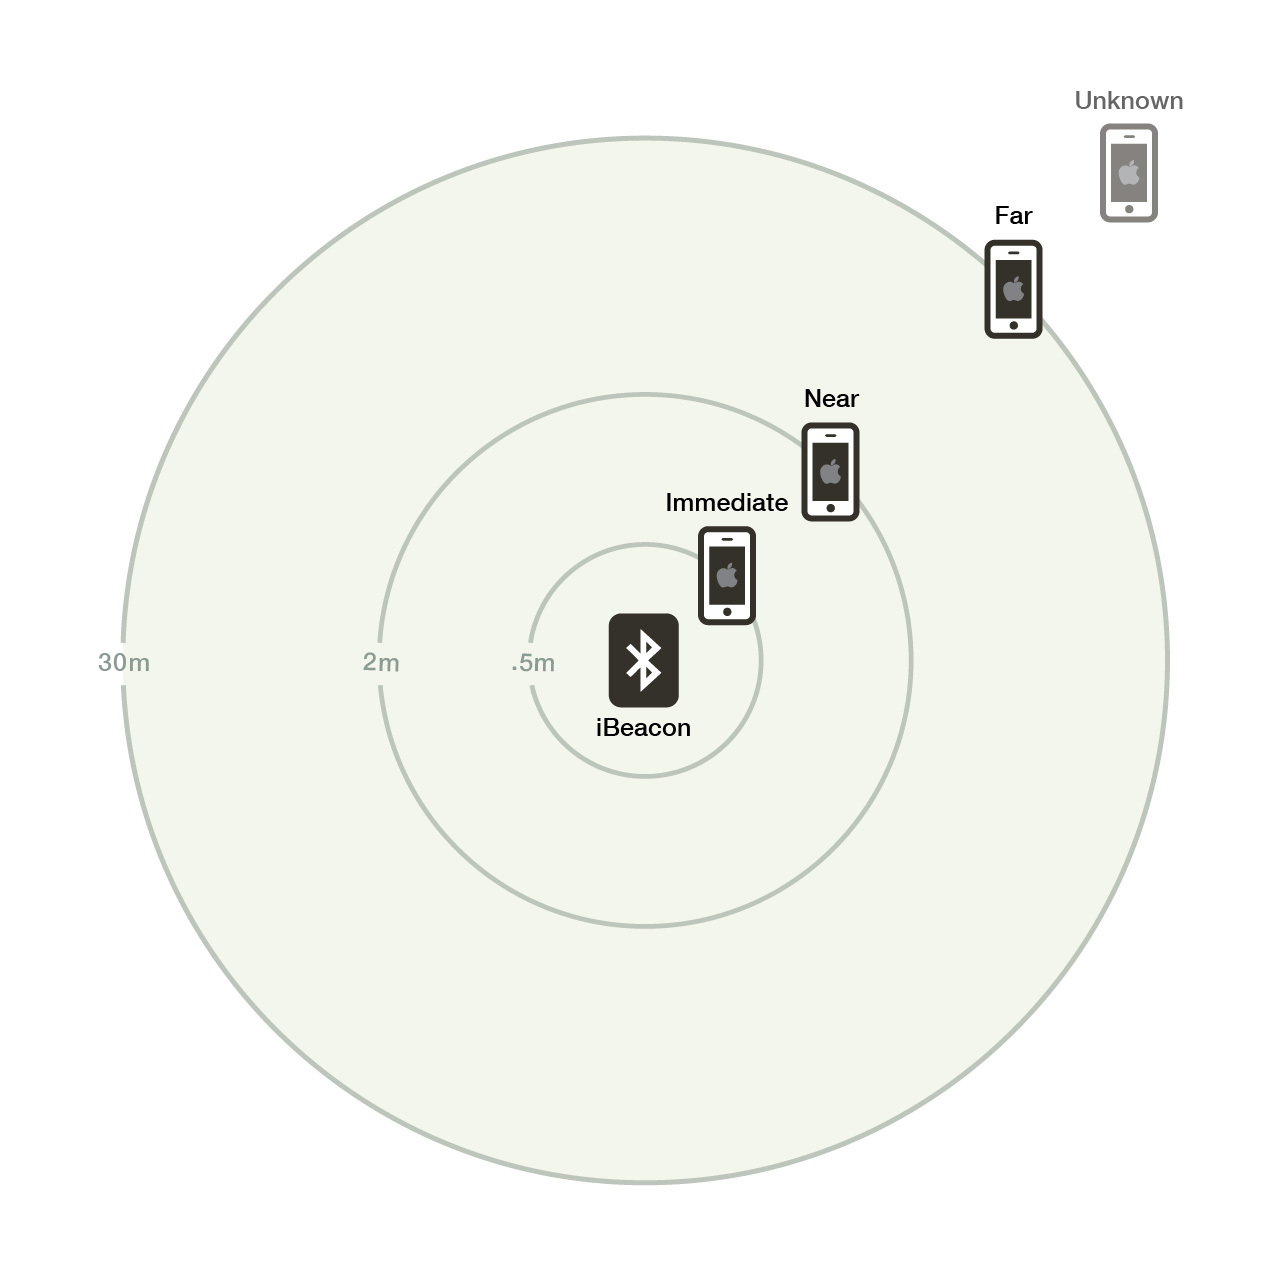
\includegraphics[height=8cm]{images/ibeacon-distance.jpg}
  \caption{Distance categories for iBeacon}
  \label{fig:ibeacon}
\end{figure}
\vspace{0.5cm}


In fact, nothing is stopping this technology from being squeezed into something as small as a typical credit card, or from being embedded in any clothing or other discrete wearable devices such fitness sensors, wristwatches or even temporary tattoos. The opportunities are indeed countless.
Whether we wear those sensors or use them in our homes and businesses (see smart thermostats, lighting and security systems for example), they can all be prepared and trained to cooperate in sophisticated and unexpected ways once the Internet knows that we are present nearby and what our intentions might be. Imagine a smart home capable of knowing when we wake up based on the activity monitor on our wrist and begin warming up the house, brewing a pot of coffee and switching off the security system. 
It is evident that with such a capacity for sensing and responding to our needs,  the Internet of things is slowly shaping a brand new world capable of being alive in ways that it has never been before.


\vspace{0.5cm}
\begin{figure}[htbp]
  \centering
    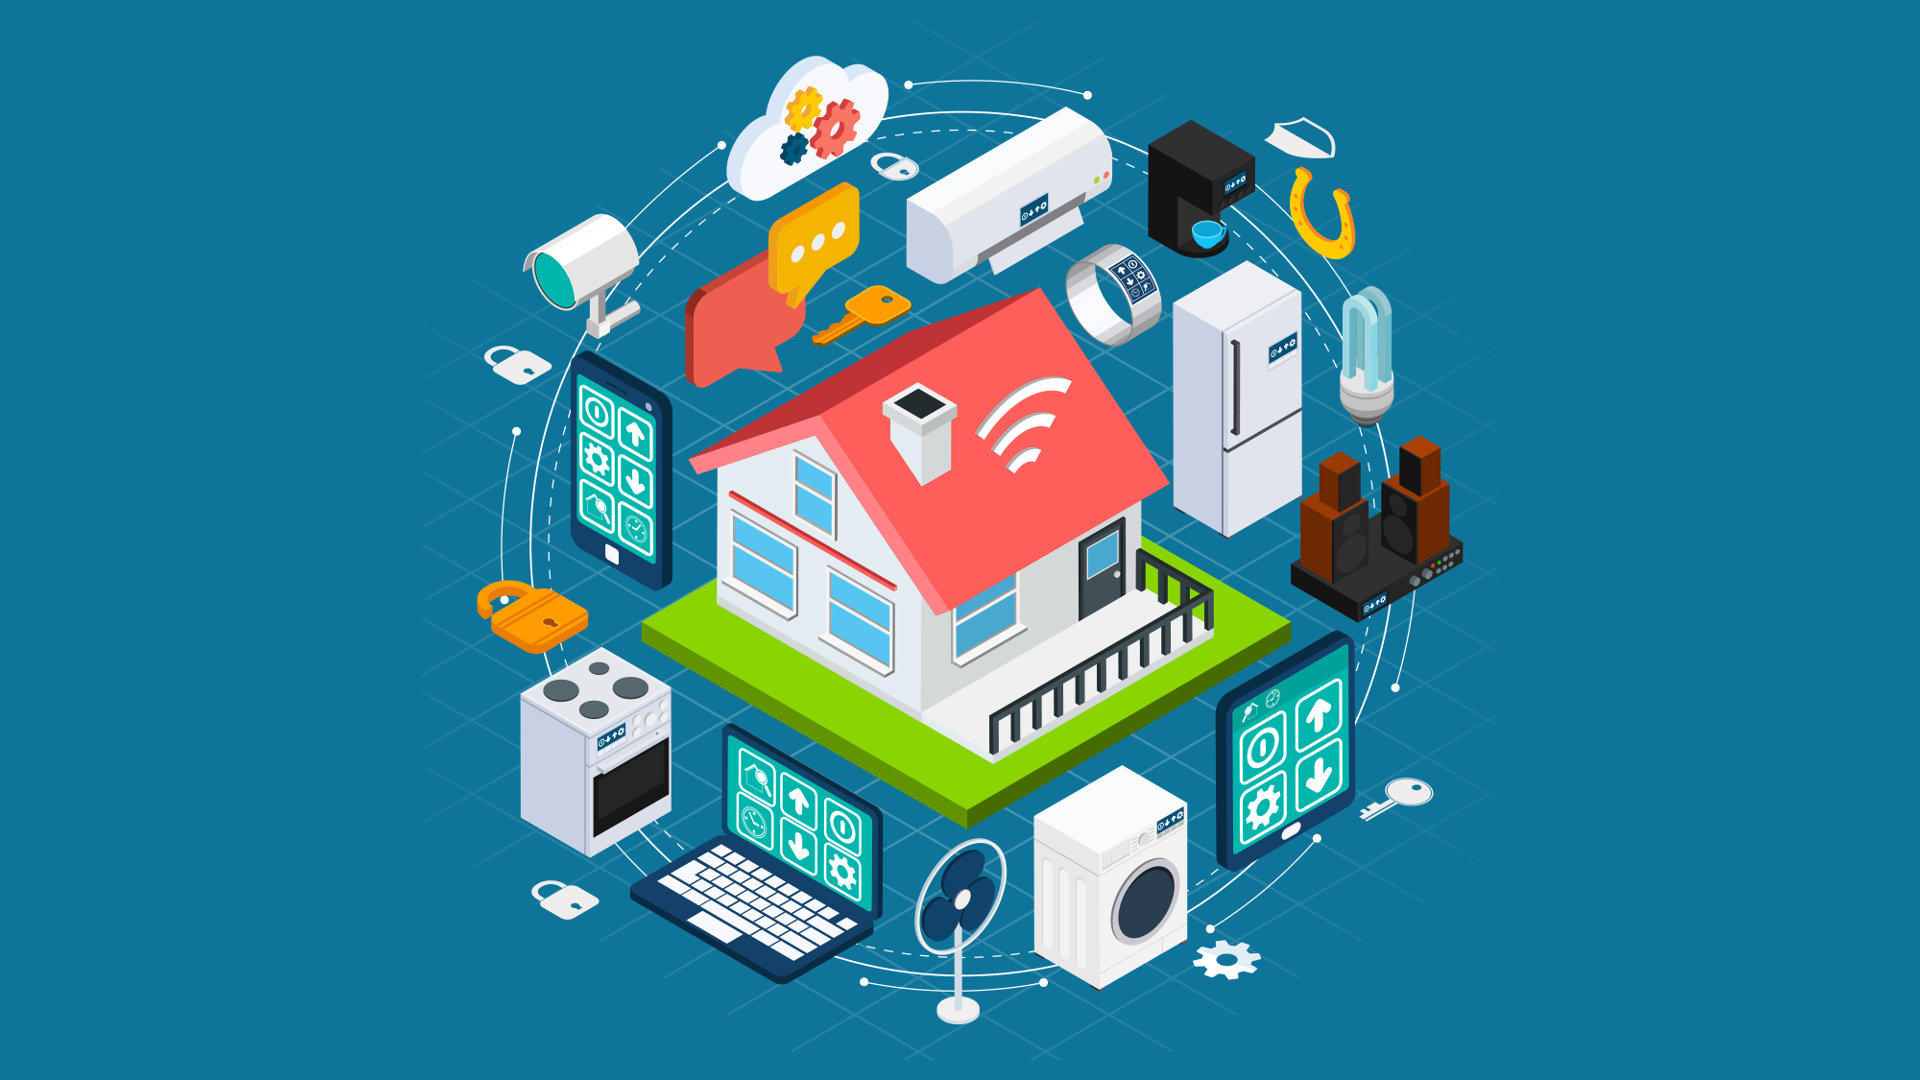
\includegraphics[height=8cm]{images/iot}
  \caption{A smart home ecosystem}
  \label{fig:iot}
\end{figure}
\vspace{0.5cm}

\section{Data and web mining}

VVery often, company management requires selecting the most adequate Business Intelligence solutions that will fit its needs in order to perform crucial strategic decisions.

One of the tools used for this particular goal is a technique called data mining, which is the result of a continuous evolution that has been occuring during the last thirty years of data review.
Up until the late 1970s, Business Intelligence decisions carried out their role through the use of standardized reports which contained simple summarized data and analysis.

In the early 1980s, companies began to query data in more detailed and complex ways. This made it easier to detect patterns based, for example, on an individual product or geographic area.

Currently, the advanced software available on the market for data mining is capable of performing real time pattern detection on a vast quantity of data thrown at it. This expedites a company’s decision making processes and the creation of robust long-term strategies.

\vspace{0.5cm}
\begin{figure}[htbp]
  \centering
    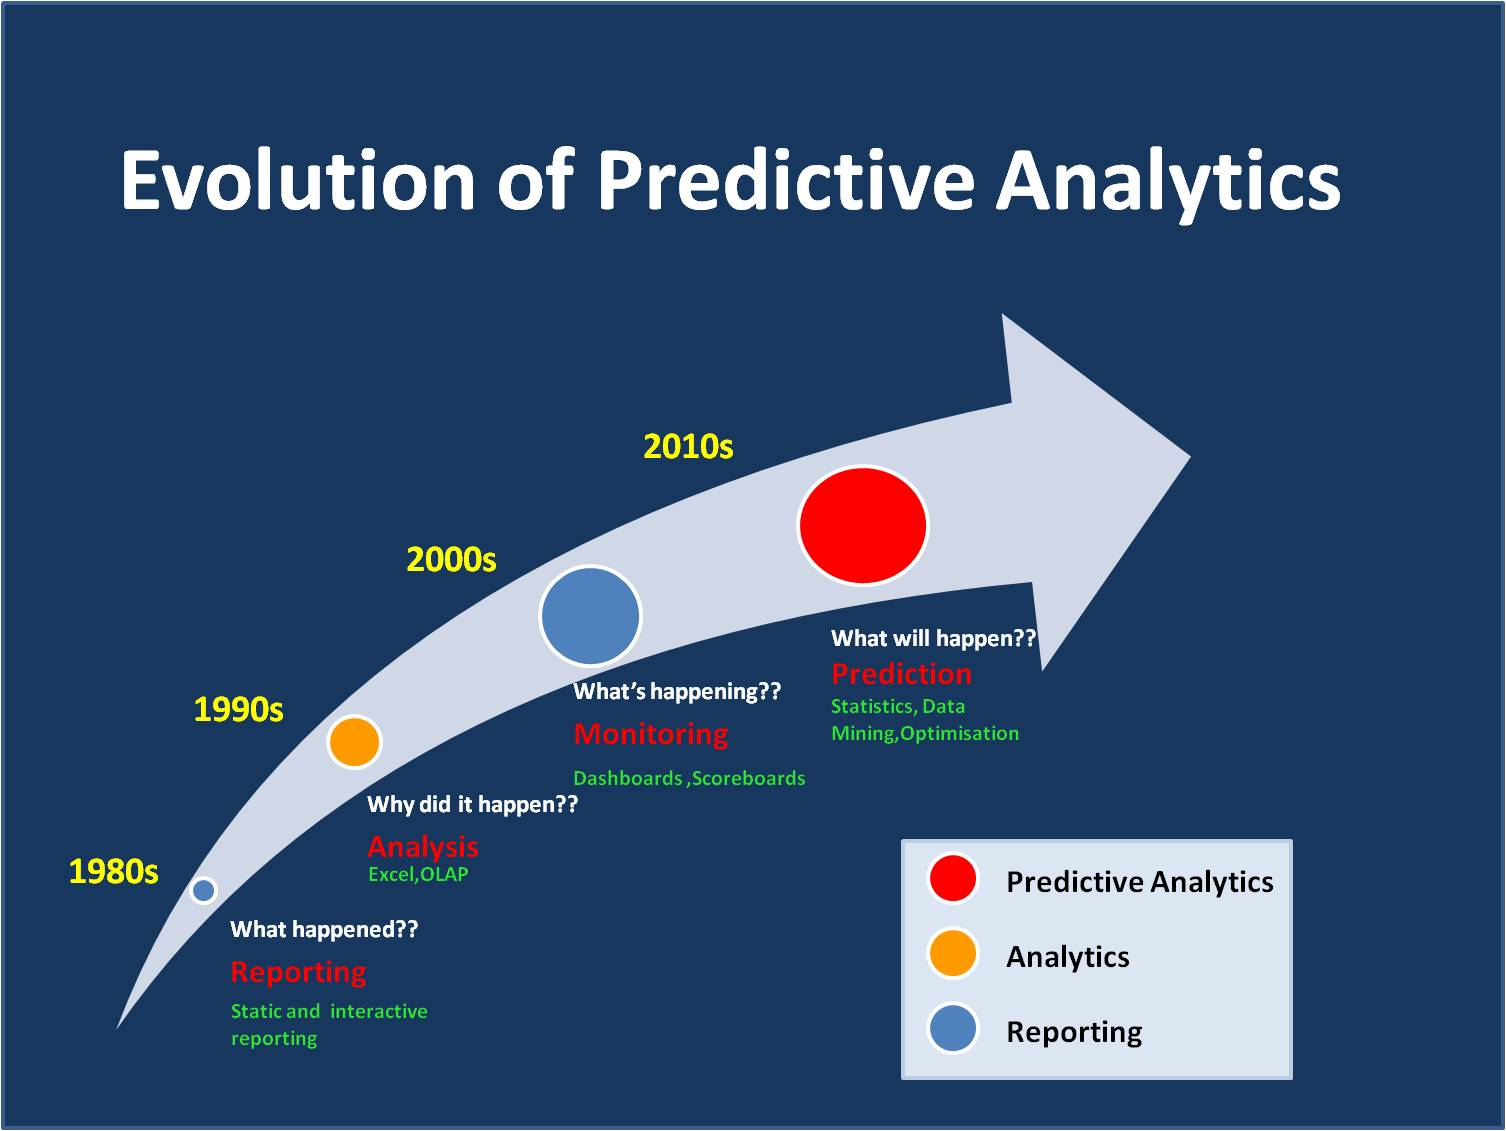
\includegraphics[height=8cm]{images/evolution}
  \caption{Evolution of Predictive Analysis over the last 40 years}
  \label{fig:predict}
\end{figure}
\vspace{0.5cm}
 

Thorough interpretation and analysis of the available data allos the data mining process to create a better overall understanding, and helps in making better decisions.

In fact, thanks to advanced examination techniques, it is possible to find hidden information, create analytical models and data groups, and identify relationships among activities while also correcting errors.

All of this certainly leads to real advantages for a company leveraging these processes, both in terms of revenue and cost. For example, on the side of income, data mining allows companies to identify and classify the best, real and potential customers, discover additional sales opportunities, increase economic productivity and find new ways and new solutions to grow. In parallel, regarding the aspect of cost, the process could maintain clientele by identifying customer loyalty elements, reducing exposure to non-payment risks and distributing resources more efficiently.

For an organization, the reasons behind using data mining may be different.
The unifying point, however, is the need to derive insight from the data that will guide the transformation, reorganization or innovation of business processes.
It is evident that decisions based on accurate and reliable knowledge are always the best. Data mining, in fact, provides exactly this type of information.
While Enterprise Resource Planning (ERP) systems improve operational efficiency, they do not provide the strategic drive for business growth or business change. Warehousing systems can efficiently store data, but they lack the tools to transform those figures into valuable information focused on reporting and answering mostly static questions such as areas where the company has sold the most. On the other side, data mining tools try to present a solution to a wider range of more interesting problems, such as why sales are not taking off as expected, why customers prefer competitors or which previous marketing campaigns had the best outcomes.

Understanding the answers to these questions means taking the right measures to improve the business’s performance.

Besides data visualization techniques, one of the most popular data mining processes on the market is based on the simplified transposition of the neural networks and the neural process of the human brain: when presented with models, the brain understands that some patterns are associated with other desired results. Similarly, artificial neural networks are capable, by learning about sets of historical data called learning sets, to generate patterns and validate them on other subsets of data called test sets. They operate iteratively by modifying patterns from time to time to reach an optimal solution, and they have the ability to evaluate and provide feedback on unknown data, thus making them very useful for forecasting and classifying knowledge. They are very often presented as a "black box" approach to data mining, and they turn out to be very useful when creating parametric models that are difficult to construct and when the emphasis is on forecasting rather than explaining complex patterns.


\vspace{0.5cm}
\begin{figure}[htbp]
  \centering
    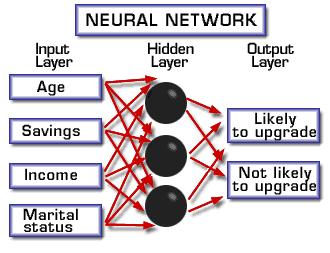
\includegraphics[height=5cm]{images/neural}
  \caption{Neural networks learn to predict outputs after proper training and weighting.}
  \label{fig:neural}
\end{figure}
\vspace{0.5cm}

After discovering what data mining means, who uses it the most, and how it is usually implemented, it is important to focus our attention on the utilization of this tool on the web and its characteristics in such an environment.

In fact, web data mining can detect behavioral models of website visitors, generate reports and implement actions based on those identified patterns.
This process is possible because website visitors often unknowingly provide information about themselves and how they respond to the content presented. Monitoring what links they click, where most of their time is spent, what search terms are entered and when the visitors leave the website are just a few appetizers of the endless stream of possible data inputs.

Some visitors also provide information about their lifestyle or personal information such as names and addresses.

Because of all of this, a thorough and adaptive analysis of this considerable amount of stored information is fundamental, and this is exactly where web data mining kicks in by helping to design the web shopper behavioral model and making valuable predictions.

One of the features that unquestionably contributes to the strength of data mining is the ability to combine emerging traffic data to the site with those related to the transactions and the profile of the buyers.

Through these combinations and by highlighting the patterns that are uncovered, it is possible to both gather complex and strategic considerations and generate predictions that may be indispensable and vital for managing a website that wants to improve its business.

\vspace{0.5cm}
\begin{figure}[!htbp]
  \centering
    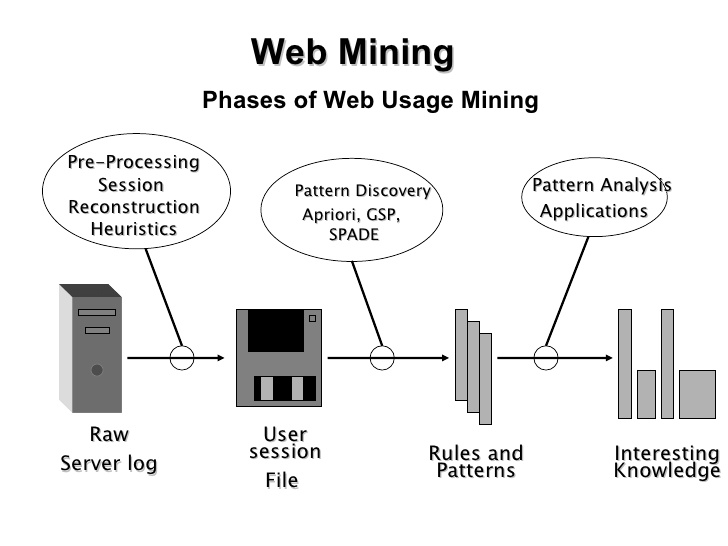
\includegraphics[height=8cm]{images/webmining}
  \caption{Phases of Web Usage Mining}
  \label{fig:webmining}
\end{figure}
\vspace{0.5cm}

Due to the heterogeneity nature of the source data, Web Mining is far from simply being an application of traditional data mining techniques. In fact, it can be categorized into three main types:

\begin{itemize}
  \item \textbf{Web structure mining}:  This focuses on analyzing and discovering useful knowledge from hyperlinks representing the structure of the Web. For example, these links allow us to detect relevant Web pages in a way similar to what search engines are already doing. Alternatively, it is possible to determine shared common interests among users and so on.
  \item \textbf{Web content mining}: The main goal of this technique is to extract valuable information or data from the content of the web pages. After doing so, it is possible to automatically classify and group this information according to topic area. While these tasks are apparently similar to those in traditional data mining, we still can discover relevant behavioral models using product descriptions, forum posts, customer reviews and much more.
  \item \textbf{Web usage mining}: This technique usually refers to the identification of user access patterns from Web usage logs once the sanitization and preprocessing of the clickstream data has occurred.
\end{itemize} 



Although the web mining process is similar to traditional data mining techniques, the data gets collected in an entirely different way. In traditional data mining, the data is often already available and stored in a data warehouse, whereas for the web counterpart, the effort for the data acquisition can be a cumbersome task, especially for web structure and content mining. This is due to the potentially high number of links and large quantity of pages to crawl.

\section{Model-driven techniques}

Software development techniques are continuously evolving while also trying to solve the principal problems that still affect the building and maintenance of software: time, costs and susceptability to errors.

On this topic, one of the latest research trends in software engineering is the Model Driven Engineering (MDE) technique, which was born as an extension of more specific approaches such as the Model-Driven Architecture (MDA) of the Object Management Group (OMG).\footnote{The Object Management Group (OMG) is an international, open membership, not-for-profit technology standards consortium, founded in 1989. OMG standards are driven by vendors, end-users, academic institutions and government agencies. } 

MDE's primary goal is to define the methodologies and techniques to support the process related to the entire lifecycle of software development through the manipulation of models.

Before proceeding further, it is beneficial to explain the difference between MDA, Model-Driven Development (MDD), MDE and Model-Based Engineering (MBE).

The first is, by all means, an OMG standard focused on software development and using a set of defined languages utilized for a specific purpose (e.g. UML\footnote{The Unified Modeling Language (UML) is a general-purpose, developmental, modeling language in the field of software engineering, that is intended to provide a standard way to visualize the design of a system.}). On the other hand, the focus of MDD is still on software development, but is independent of mandatory language constraints to perform its tasks.
MDE, as a superset of MDD, does not only drop the software-related restrictions, but it unties itself from a particular development process, therefore expediting the definition of model driven processes to facilitate a complete software engineering process. 
Finally, we use MBE to refer to a softer version and a superset of MDE where models still play an important role, but are not the central artifacts of the development process. (e.g. blueprints or sketches of the system handed out to programmers directly without automatic code generation) ( Figure \ref{fig:mda} ).

\vspace{0cm}
\begin{figure}[htbp]
  \centering
    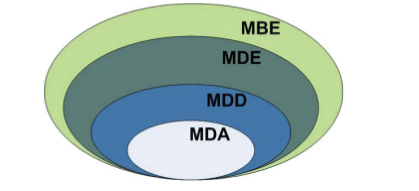
\includegraphics[height=4cm]{images/mda}
  \caption{Relationship between the different MD* acronyms.}
  \label{fig:mda}
\end{figure}
\vspace{0cm}

The model is at the center of any MDE process and, to be considered as such, the modeling language that generated it needs to have well-formalized syntax and semantics. This is a fundamental condition for the automatic transformation of models. In fact, the model represents the system and constitutes an abstract and conforming formalization to a particular language. Such a language is often tailored to a certain domain and is often called Domain-Specific Language (DSL). 

The advantages of using the model driven approach rely on the consideration of the generating language as a type of scheme that is also fully modelable through a formal and abstract definition known as the meta-model. In fact, the model must represent an abstraction of the concepts of the system that needs to be built, while also respecting a meta-model likewise determined by the application domain.

This reasoning can be further iterated up to the determination of a model for the representation of languages used to formalize other languages (the meta-meta model).

Because of the above, model-driven approaches are often defined by models on a stack basis as shown on Figure \ref{fig:mde}.

\vspace{0cm}
\begin{figure}[htbp]
  \centering
    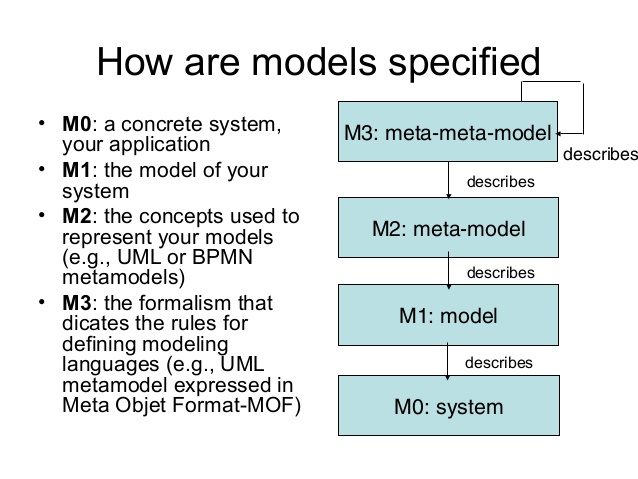
\includegraphics[height=8cm]{images/mde}
  \caption{Models stack}
  \label{fig:mde}
\end{figure}
\vspace{0cm}

One of the most commonly used techniques in MDE is the automatic model generation based on the definition of a set of automatic transformations defined by the starting and target languages. In a nutshell, the MDE approach consists of:

\begin{itemize}
  \item \textbf{Models Generation}, based on modeling stacks definition supporting meta-modelling methods where lower-level models comply with what is specified by higher-level models.

  \item \textbf{Models Manipulation} performed through transformations expected to generate destination models which conform to destination meta-models when provided with source models that conform to source meta-models.
\end{itemize} 

In summary, MDE techniques allow, on the one hand, for the management of the complexity of a system by ensuring increased productivity, and for quality improvements by promoting a higher level of abstraction and reuse, on the other. This result is achieved through a process of engineering, both for the languages and the transformations involved: they are, in fact, the basis of a system’s development process because they represent the transition from higher-level models into lower-level ones until they can be made executable using either automatic code generation or model interpretation.

%\addcontentsline{toc}{chapter}{}


\clearpage

 % !TEX root = Tesi.tex
\chead{}
\chapter{State of the art}

\section{IoT Devices : RFID, NFC, Beacons and Sensors}

The IoT can be used in a variety of fields: personal and health applications; employments in the field of business and enterprise; use in smart cities and in the environmental field. The field of health and care of the person can have many positive effects using data from sensors and RFID tags that can be placed on medications, on machines used for analysis and medical instruments. It will be possible to get it the results of the most accurate and reliable examinations, to monitor in real time the state of health of people, schedule more medical checkups. From the business point of view, IoT technology will improve efficiency: yes will reduce costs for the production process, logistics and warehouse management, thanks to the vast amount of information collected. In addition, consumers may have more information about the products and their origin can be prevented monitoring the "state of health" of products, the greatest traceability will ensure greater transparency and assistance. Another important aspect is the impact of ICT in smart cities and domotics: By getting information in cities, these can be more efficient by improving transport and safety, reducing costs and saving time and energy, from fueling to heat residential homes for urban displacements. Environmental protection can also derive various benefits from IoT technologies: in fact it is possible levels of pollution can be monitored through the information available present in the environment and promptly intervene where necessary, saving on the costs of maintenance and regulation of sensors

\section{Big Data and Predictive Analysis applications}

The concept of Big Data relates directly to the Internet of Things: IoT devices are indeed capable of collecting terabytes of data in a short amount of time, therefore being proficient a interpreting and analyzing such information is quite critical.

It's important to notice not only IoT devices are players capable of generating profiling data at such an incredibly high rate;  as per introduced in chapter \ref{section:data-web-mining} the modern Web represents another essential data source in this paradigm: social networks, for example, are capable of producing an endless stream of data describing user preferences and behaviors at any time.

This vast volume of data available to analyzers is behind the term Big Data which can be taught as a massive dataset, growing at a very high velocity in numerous formats from a variety of different origins.

To obtain business value from this amount of information, companies necessitate algorithms and solutions fitted to efficiently process, validate and give credibility to it, solutions beyond traditional systems currently used for managing and storing information, with high power and high calculation inclination that are efficient for sorting data in a structured and meaningful manner to detect relationships and patterns.

This new approach to data management differs from what companies used to do in the past when priorities were bound to an IT level governance only and they were solely accessed by a restricted set of users. 

It also becomes vital for a company to quickly and correctly identify new sources of big data when they become available on the market incorporating them into the data management platform following a constant continuous improvement logic.

It's quite hard to estimate in advance the added value brought by the Big Data analysis to the various application disciplines in which they can be applied, but they certainly warrant an improvement of the quality of the forecasts offering useful tools to take more prudent decisions supported by more robust empiric evidence.

In fact, Big Data analysis constitutes a fantastic instrument in the field of the decision-making throughout the whole organization pipeline minimizing the risks and reducing the errors caused by possibly wrong human intuitions at any level. For example, the Marketing department could potentially leverage big data for increasing marketing intelligence predicting customer interests while Logistics can utilize Big Data to better forecast product stock refurbishment or Operations can use it to optimize production requests.

\vspace{0.5cm}
\begin{figure}[htbp]
  \centering
    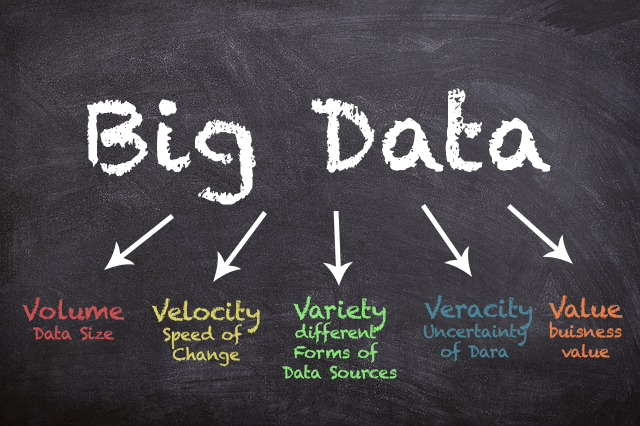
\includegraphics[height=8cm]{images/bigdata.png}
  \caption{The five fundamental Vs of big data }
  \label{fig:bigdata}
\end{figure}
\vspace{0.5cm}

In a nutshell, the potential applications mentioned above represent the core of the predictive analysis notion: the practice of extracting information from Big Data with the goal of determining patterns and predicting future outcomes and possible trends. 

It's important to notice that this kind of analysis does not offer a precise statement of what will happen in the future but rather they forecast what might occur with an acceptable level of reliability including what-if scenarios and risk assessment.

Focusing on the Marketing intelligence example mentioned above the benefits of using Predictive Analysis are immediate to understand. Indeed, it is one of the possible applications digital companies are embracing with the fastest rate nowadays, mostly because it allows them to offer better and more constructive experiences to the customers on every possible point of contact between the business itself and the clients with the goal of increasing customer loyalty and, naturally, incomes.


In detail, this process takes place using sophisticated algorithms and mathematical models on top of the big datasets of customers activity accessible from Big Data sources; eventually, this data gets sanitized, structured and filtered and finally grouped in a meaningful way. 

The behaviors and patterns of interaction detected by this process can indicate, for example, a more appealing product offer with a major chance of conversion for a particular customer profile segment.

\vspace{0.5cm}
\begin{figure}[htbp]
  \centering
    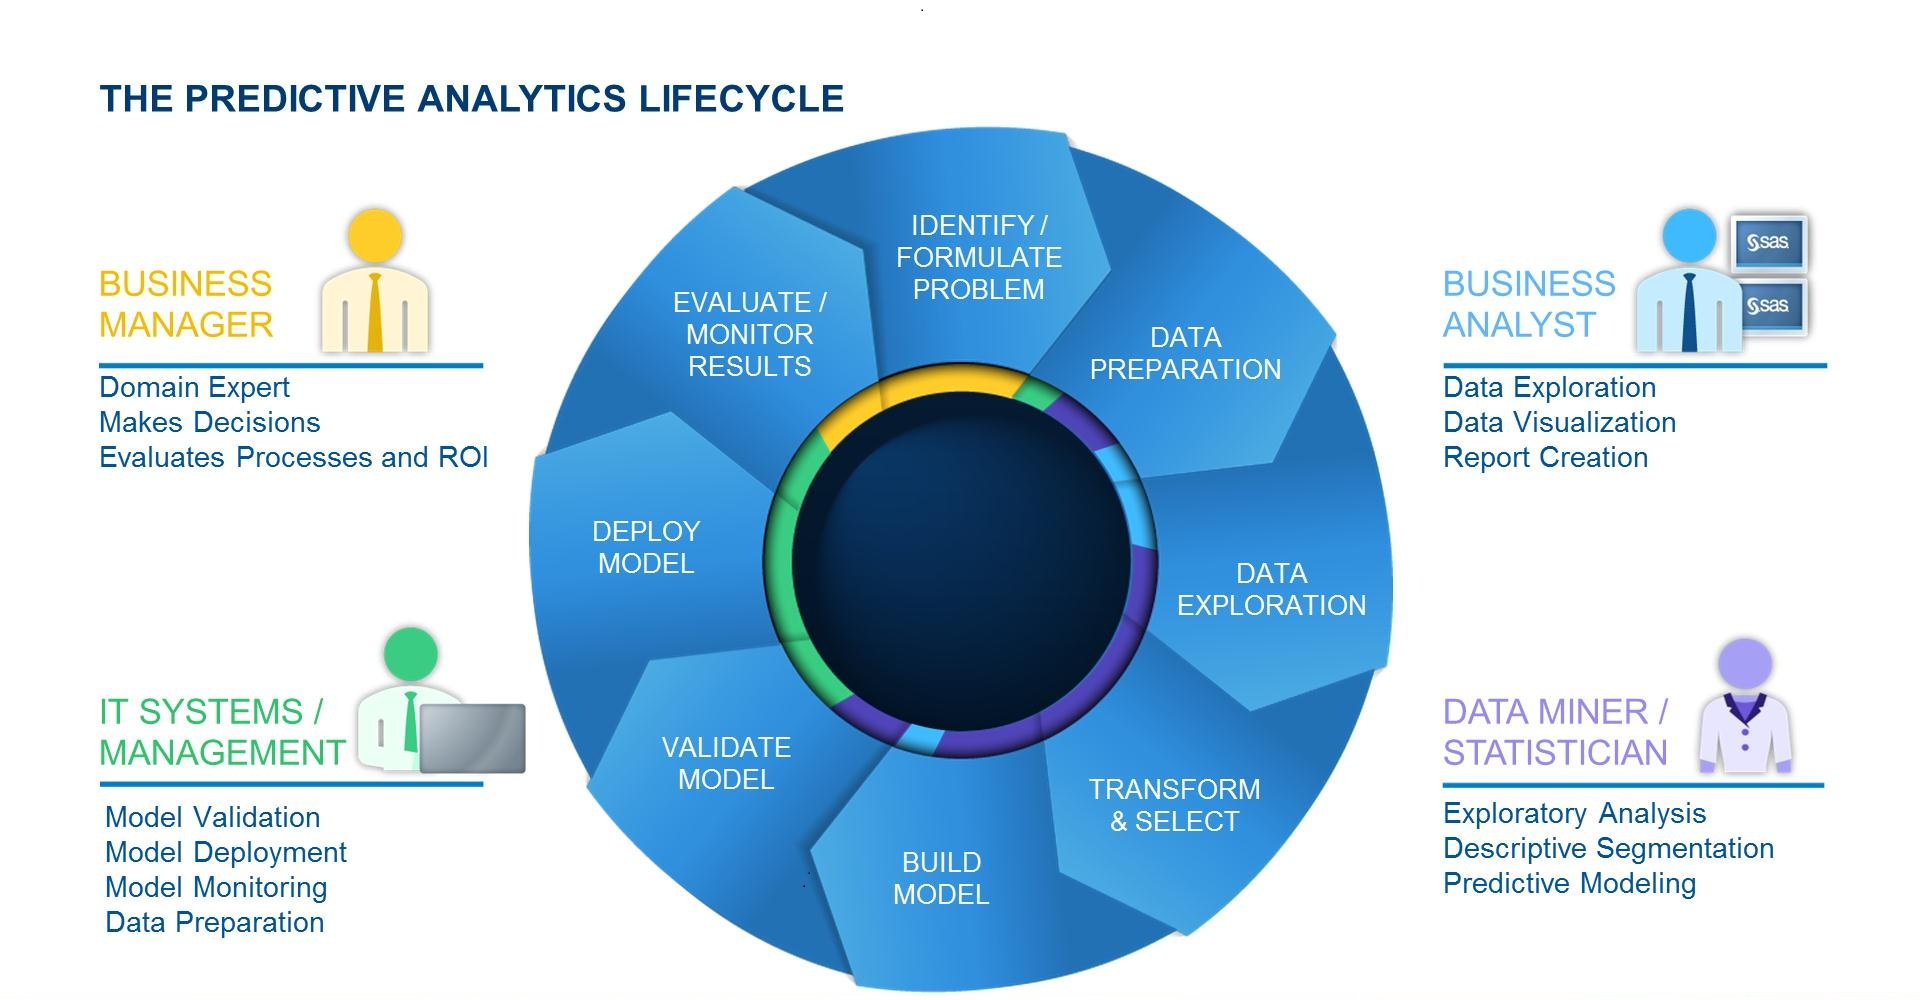
\includegraphics[height=8cm]{images/pa-lifecycle.jpg}
  \caption{The predictive analysis lifecycle }
  \label{fig:bigdata}
\end{figure}
\vspace{0.5cm}

As mentioned above different typologies and techniques are used to perform this type of analysis for behavioral prediction, these are the most important ones :



\begin{itemize}
    \item \textbf{Clustering or Unsupervised learning}:  This methodology groups similar individuals and identifies with high precision the enterprise's customer base. The algorithm processes hundred of attributes until it identifies the discriminating ones for a more efficient segmentation: the underlying idea is that several statistically significant groups behave in the same way. 

    The clusters obtained with this process are similar to groups determined through a priori segmentation; the fundamental difference between the two methodologies is that, while segmentation involves assigning customers to previously identified groups, clustering allows to distinguish the natural disposition of individuals in the different groups based solely on data and not preventive attributes definition. 

    Clusters can be of different types depending mostly on the criteria by which customers are grouped : product-based clusters, for example, gather all customers who tend to buy products or combinations of several products in the same category, brand-based clusters, on the other hand, focus on customers who prefer certain brands instead of others while behavior-based clusters combine consumers with similar buying behaviors, helping the marketing manager to identify the most appropriate way to address each of them.

    \item \textbf{Propensity models or Supervised learning}: This technique is based on probabilistic models using advanced machine learning techniques such as neural networks, logistic regression, random forest, and regression trees. The main purpose of these procedures is to predict future customer behavior based on past examples. Over time, these algorithms become more efficient, hardening forecasts with more data.

    \item \textbf{Reinforcement learning and Collaborative filtering}: This highly used technique in making predictions has major applications, one of the most famous one being the recommendation suggestion which offers tips on which products to buy. The recommendations are targeted and tailor-made for the client and they are obtained taking into consideration the entire relationship between customer and brand. Respectively they can upsell for higher value products, cross-sells to same category items or dynamically link other products based on the bought-together association.
  \end{itemize} 


 



%\addcontentsline{toc}{chapter}{}

\clearpage

 % !TEX root = Tesi.tex
\chead{}
\chapter{Data acquisition}

The evolution of the Internet and the amount of data available from web usage mining and IoT devices have led to an enormous proliferation of the accessible information as per described in the previous sections.  In this chapter, we focus on describing the possible channels of acquisition of customer behavioural data in both the virtual and the physical world. This valuable information represents the milestone of the journey towards the enhancement of the eCommerce experience for its users, and aims at addressing some of the weaknesses of the standard approaches for web personalisation.

Before we can efficiently represent content visualised on user interfaces, navigation paths and user-triggered events on a web application, we need to take a little detour briefly introducing a standard modeling language able to shape such interactions. This language will be analysed in detail in the following sections.

\section{The IFML language}
\label{the-ifml-language}

The Interaction Flow Modeling Language (IFML)\cite{IFML-1, IFML-2} is designed for describing and controlling the behaviour of front-end software applications. IFML brings several advantages to the development process, such as promoting the separation of concerns between roles and increasing the overall understanding of the product for non-technical stakeholders. That can be achieved because IFML supports formal specification for interface composition, user interaction, and event management independently of the implementation platform. This language was adopted as a standard by the Object Management Group (OMG) in March 2013.

IFML supports the following concepts: 

\begin{itemize}
  \item \textbf{The view structure} describes \textit{ViewContainers}, their nesting relationships, their visibility, and their reachability.
    
  \item \textbf{The view content} manages \textit{ViewComponents}, i.e., content and data entry elements contained within ViewContainers.
  
  \item \textbf{The events} defines the \textit{Events} that may affect the state of the user interface. \textit{Events} can be produced by the user interaction, by the application, and by an external system.

  \item \textbf{The actions} triggered by user events. The effect of an \textit{Event} is represented by an \textit{InteractionFlow} connection, which connects the event to the \textit{ViewContainer} or \textit{ViewComponent} affected by the \textit{Event}. The \textit{InteractionFlow} expresses a change of state of the user interface: the occurrence of the event triggers a change in the state that produces a transition in the user interface.
  
  \item \textbf{The navigation flow} indicates the effect of an Event on the user interface.

  \item \textbf{The data flow} indicates the data passed between \textit{ViewComponents} and \textit{Actions}.
  
  \item \textbf{The parameter binding} illustrates the input-output dependencies between \textit{ViewComponents} and between \textit{ViewComponents} and \textit{Actions}. 


\end{itemize} 

\vspace{0.5cm}
\begin{figure}[H]
  \centering
    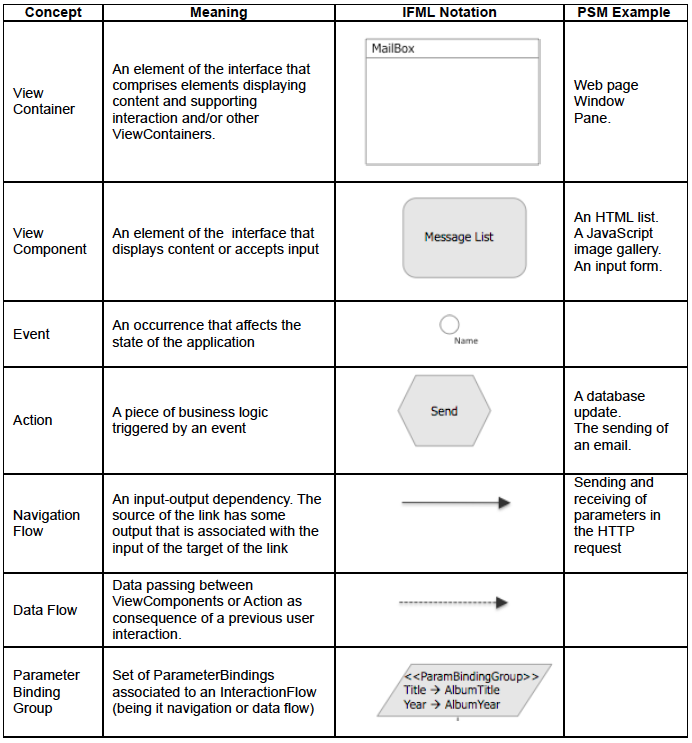
\includegraphics[width=10cm]{images/ifml.jpg}
  \caption{Main IFML concepts and notations.}
  \label{fig:ifml}
\end{figure}
\vspace{0.5cm}

\newpage

\section{Web navigation profiling}
\label{navigational-modeling-for-the-web}
The front-end of eCommerce websites is usually built using shared and reusable components (forms, list views, detail views, etc.), which have a specific and expected behaviour.
For example, product lists and grids show users record details and create possibilities for interaction. Similarly, ``add to cart" buttons are placed on strategic points within product pages to trigger a specific user action.
These interactions and any other user action withing the website can be represented using the IFML notation.

To demonstrate the versatility and adaptability of this modeling language, we introduce a real-life example which will serve as reference from this chapter forward: an online boutique website called \textit{``Madison Island"} and specialised in fashion items running on an eCommerce platform.

Madison Island presents all the features of a typical digital store including catalogue navigation, product searching, customer account, shopping cart, and order processing. 

\vspace{0.5cm}
\begin{figure}[htbp]
  \centering
    
\includegraphics[width=12cm]{images/home.png}
  \caption{Madison Island digital store homepage}
  \label{fig:home}
\end{figure}
\vspace{0.5cm}


Figure \ref{fig:home} shows the home page of the website. In this section, the user can select one of the product categories, access his customer area, switch the language of the website, search for an item or go directly to the shopping cart. 

In the following subsections, we analyse some scenarios related to users navigational behaviours, exposing both their representation in IFML notation as well as the log entries in the application server associated with those representations.

\newpage
\subsection{The product page journey}
\label{the-product-page-journey}

Starting from the homepage, the user can interact with the navigation menu by choosing from a set of available categories.  (Figure \ref{fig:navigation})

\vspace{0.5cm}
\begin{figure}[H]
  \centering
    
\includegraphics[width=9cm]{images/madison/navigation.png}
  \caption{Navigation menu}
  \label{fig:navigation}
\end{figure}
\vspace{0.5cm}

Depending on the category display mode, a category page can show users either a list of links to children categories or a set of products. In the former case, children categories work as transitional pages that help further filtering products (Figure \ref{fig:category-display-modes}).


\vspace{0.5cm}
\begin{figure}[H]
  \centering
  \subfloat[Category listing]{{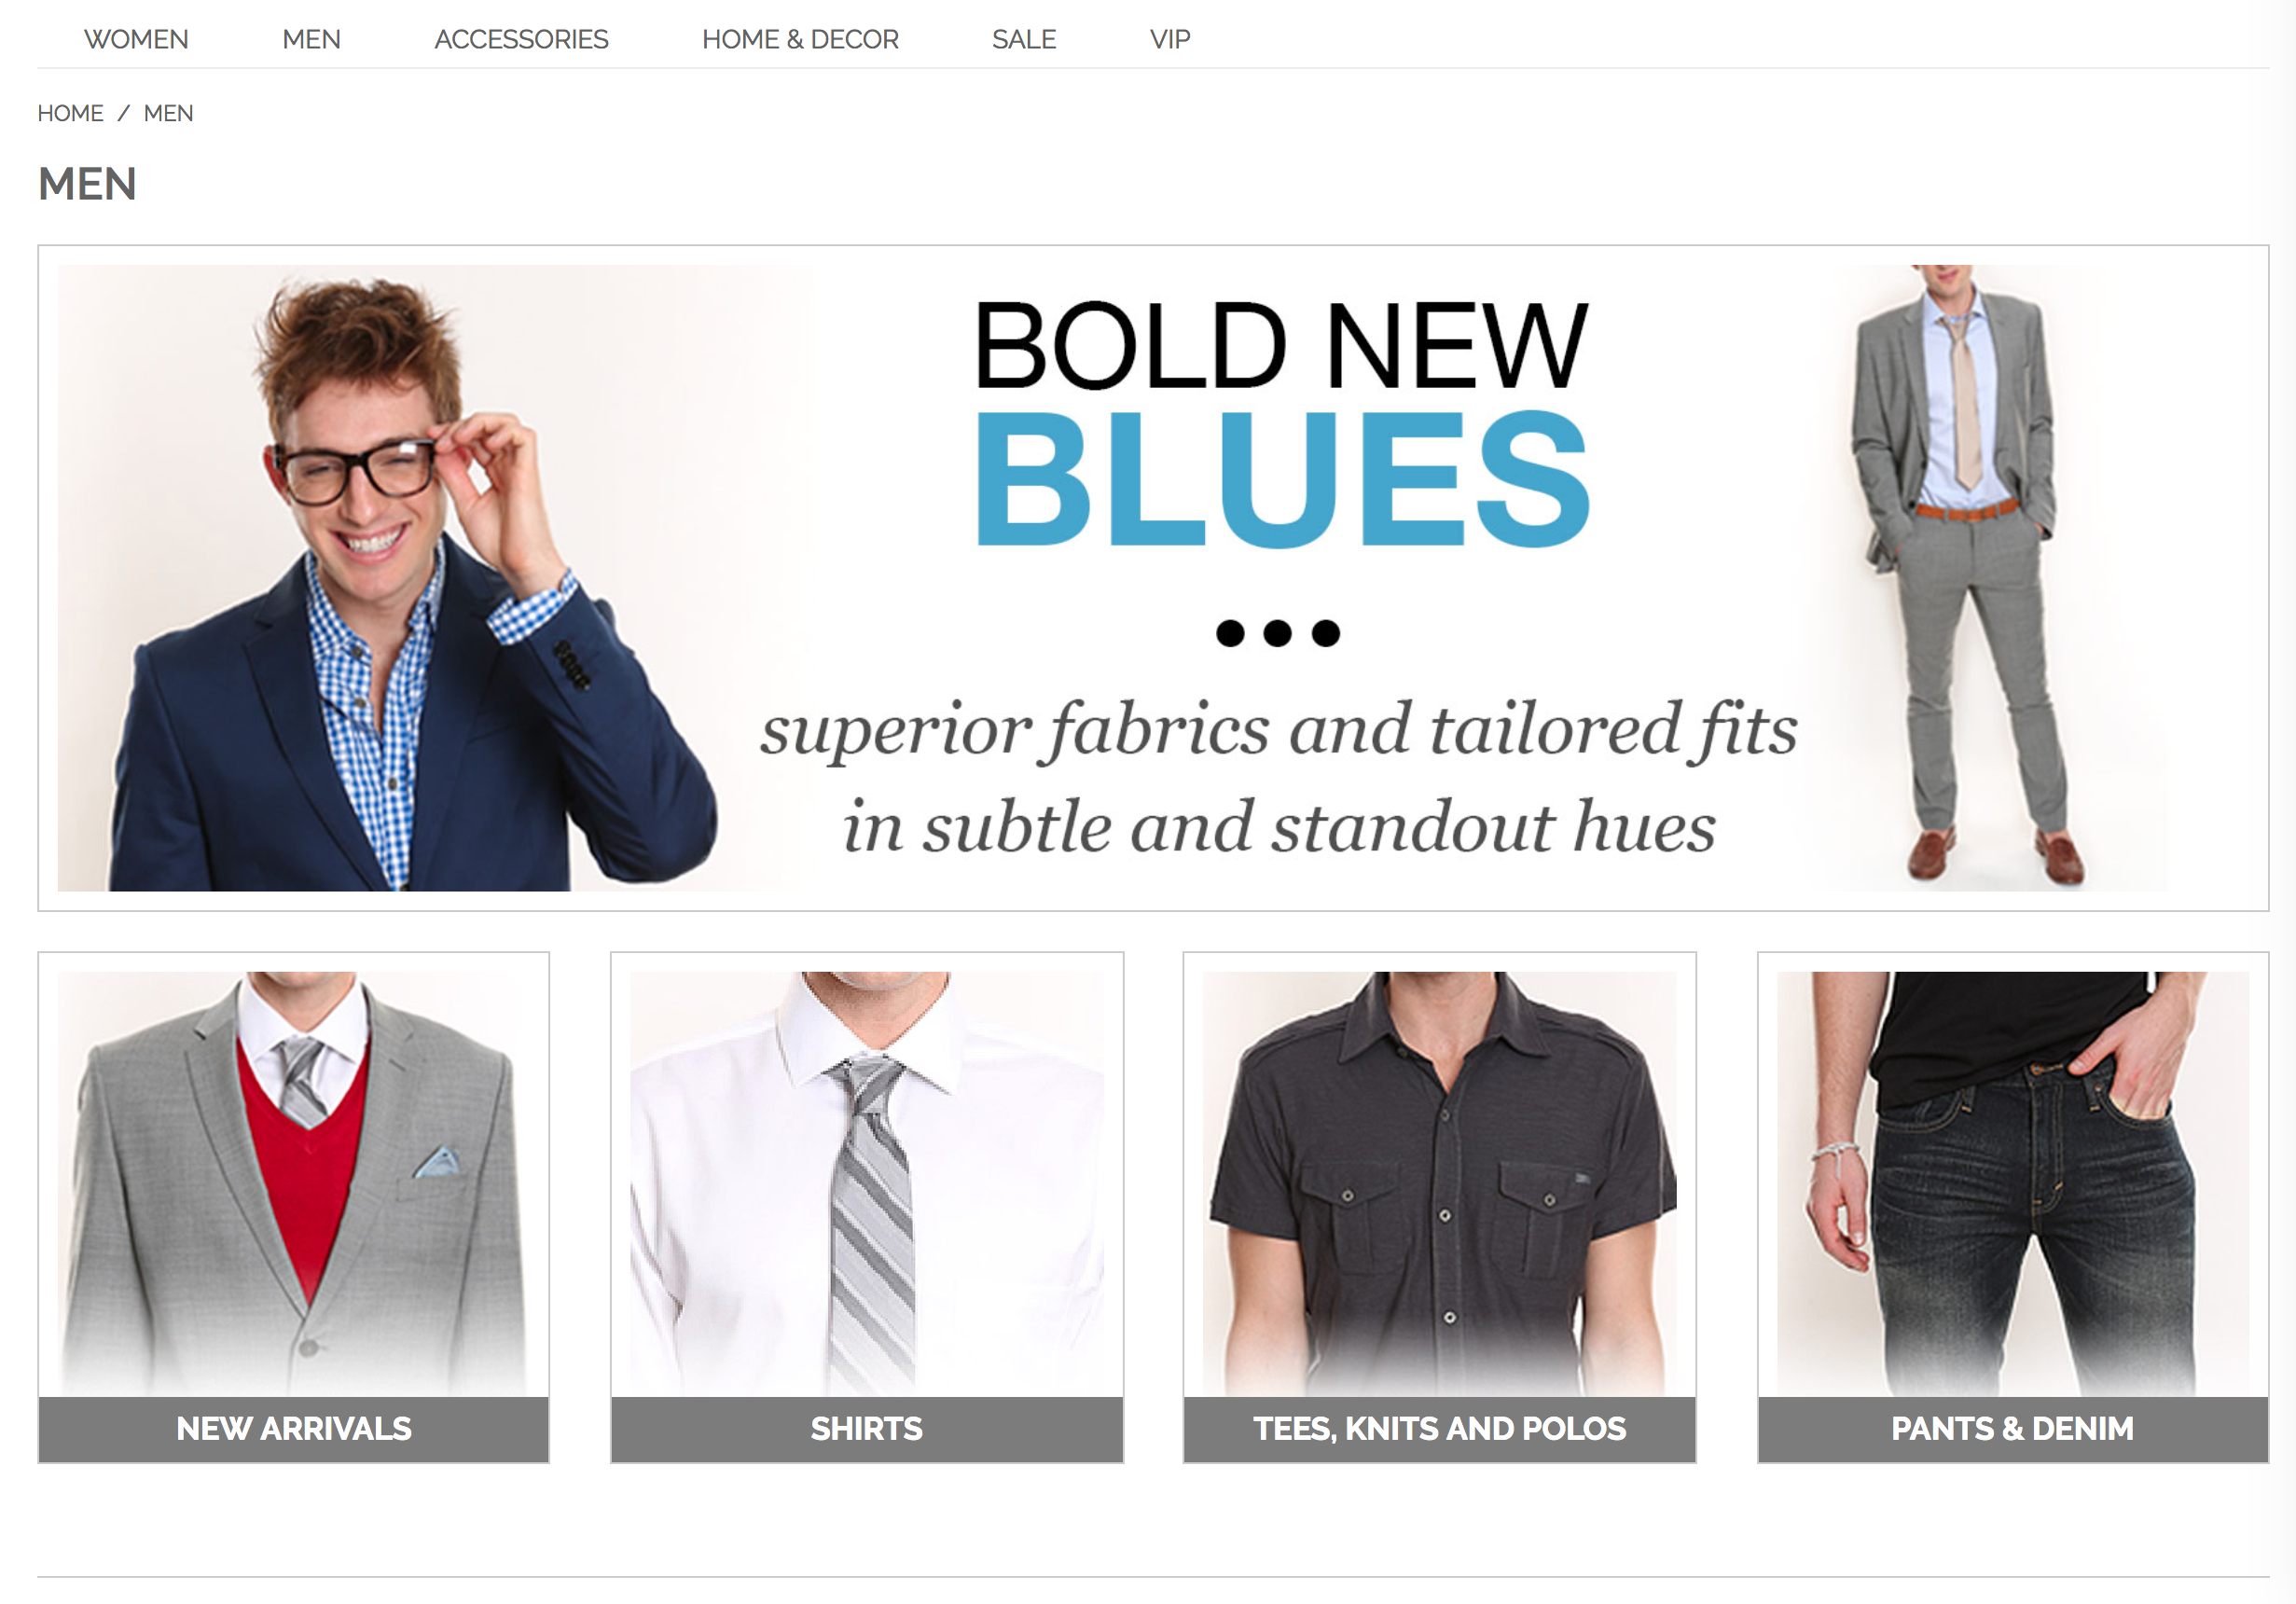
\includegraphics[width=7cm]{images/madison/category-cms.png} }}%
  \qquad
  \subfloat[Product listing]{{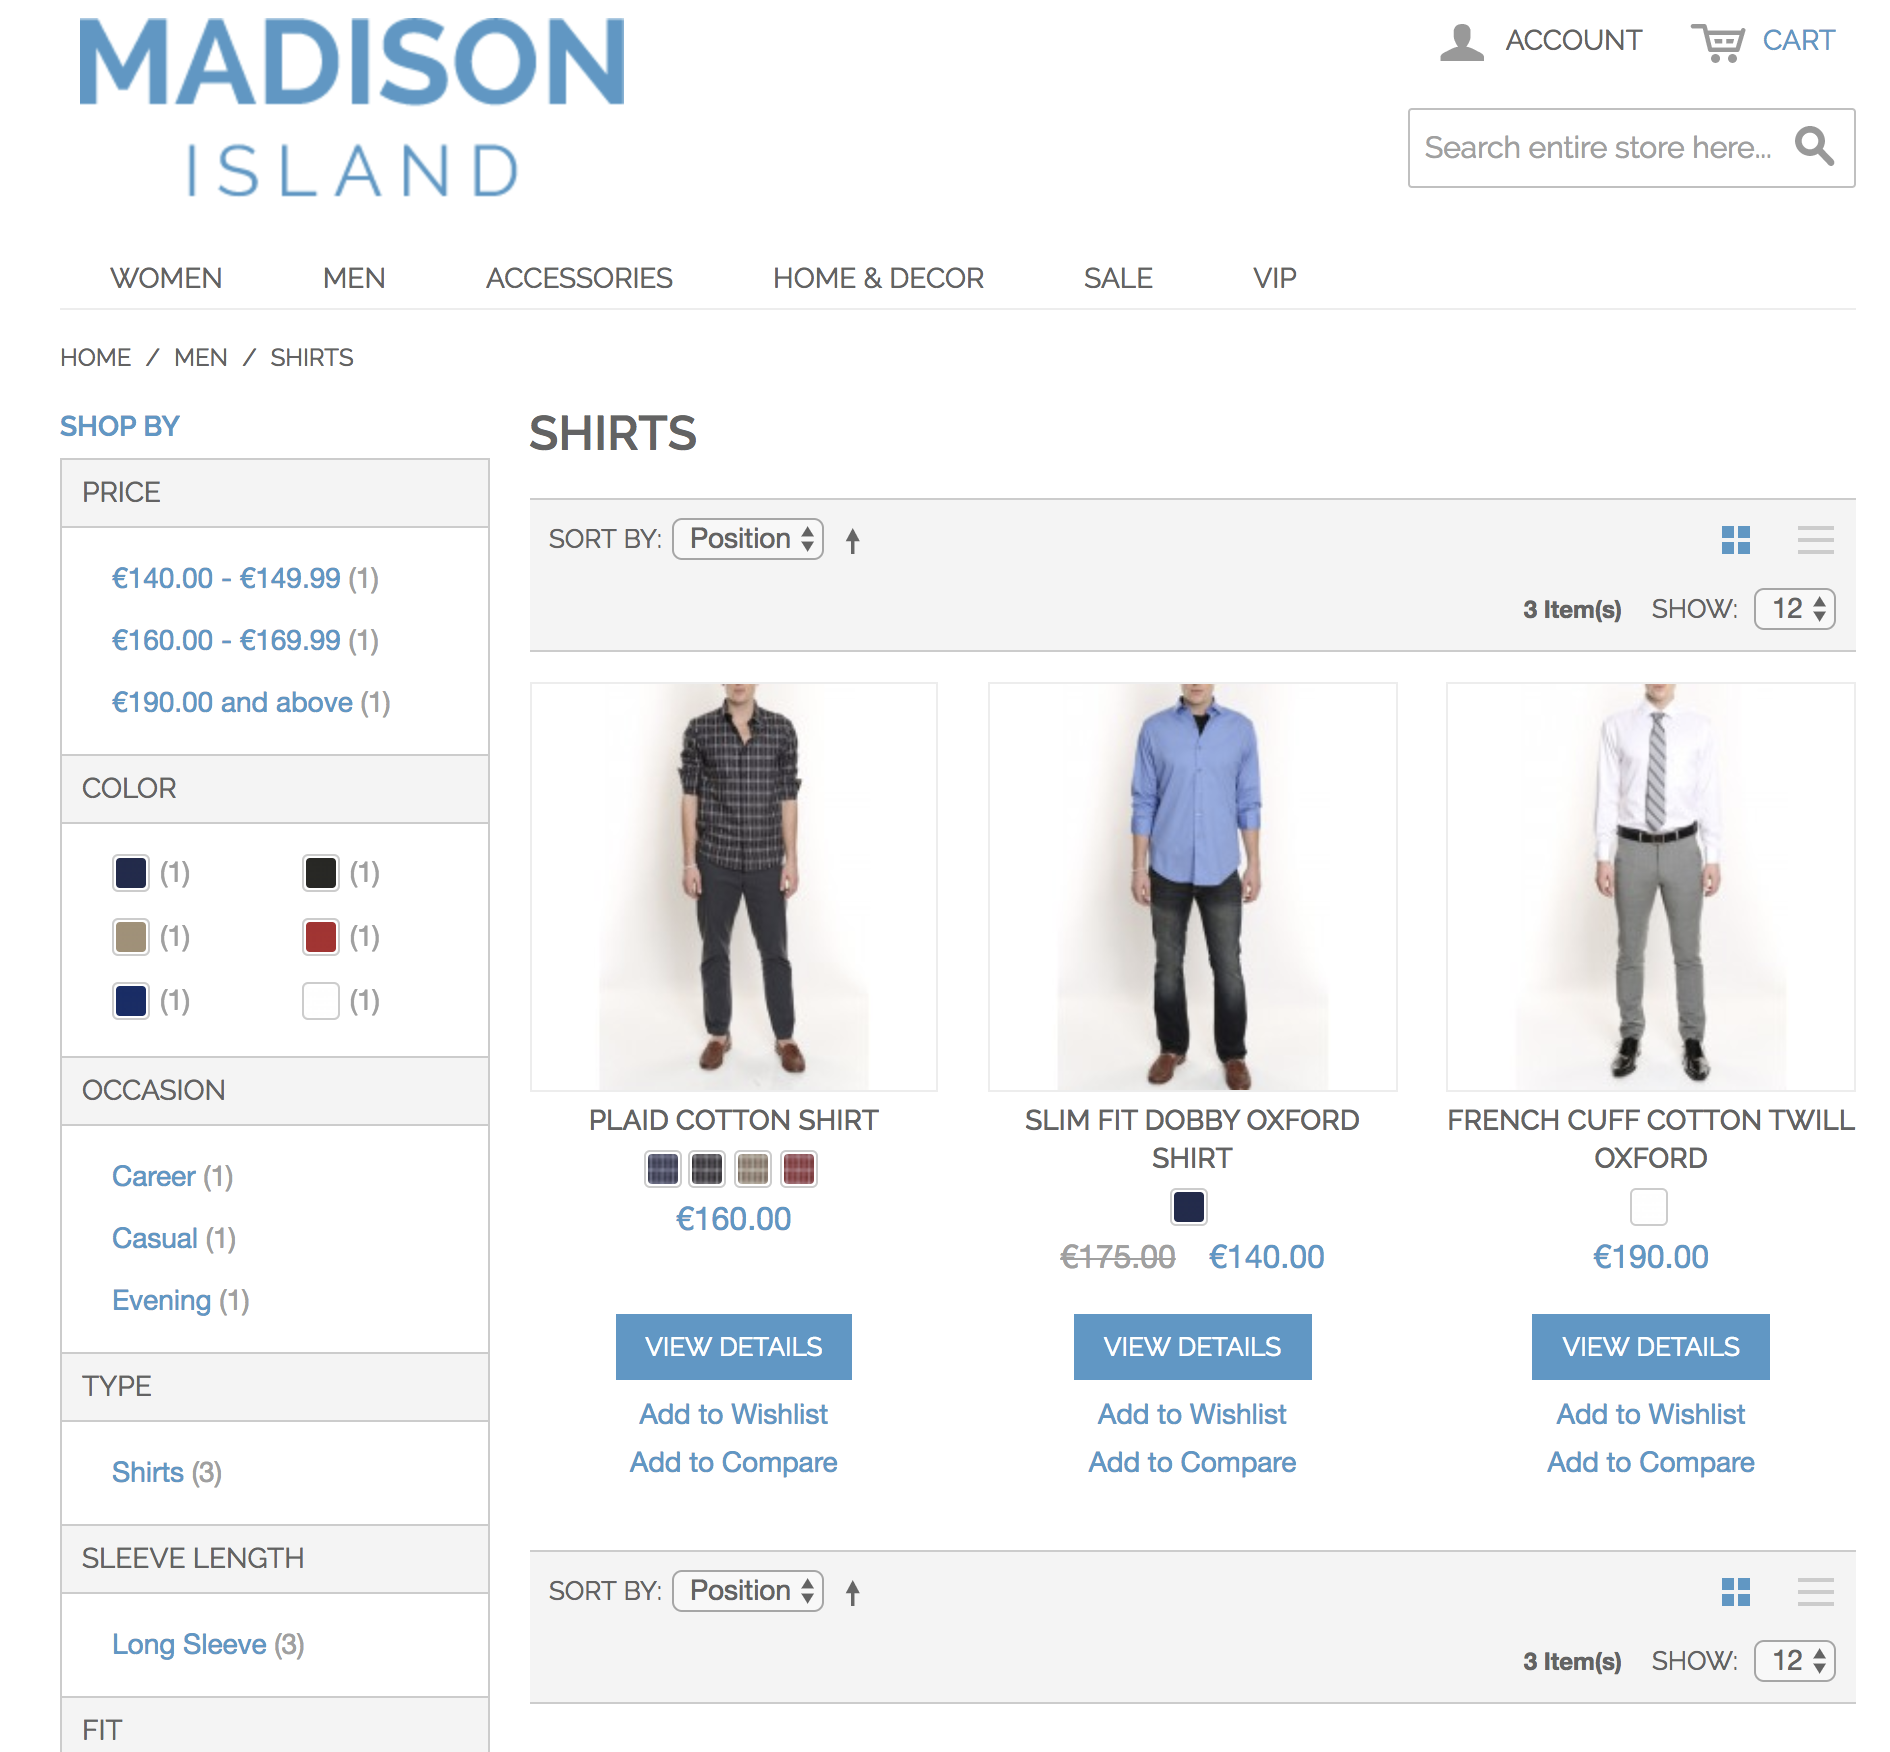
\includegraphics[width=7cm]{images/madison/products-list.png} }}%
  \caption{Different category page view modes}%
  \label{fig:category-display-modes}%
\end{figure}
\vspace{0.5cm}

Finally, from the product listing screen, the user can access any of the product detail pages by clicking on the \textit{``View Details"} button placed below the selected product thumbnail. The following image illustrates the product page seen when the user clicks on \textit{``View Details"} of \textit{``Plaid Cotton Shirt"} (Figure \ref{fig:product-detail}).


\vspace{0.5cm}
\begin{figure}[H]
  \centering
    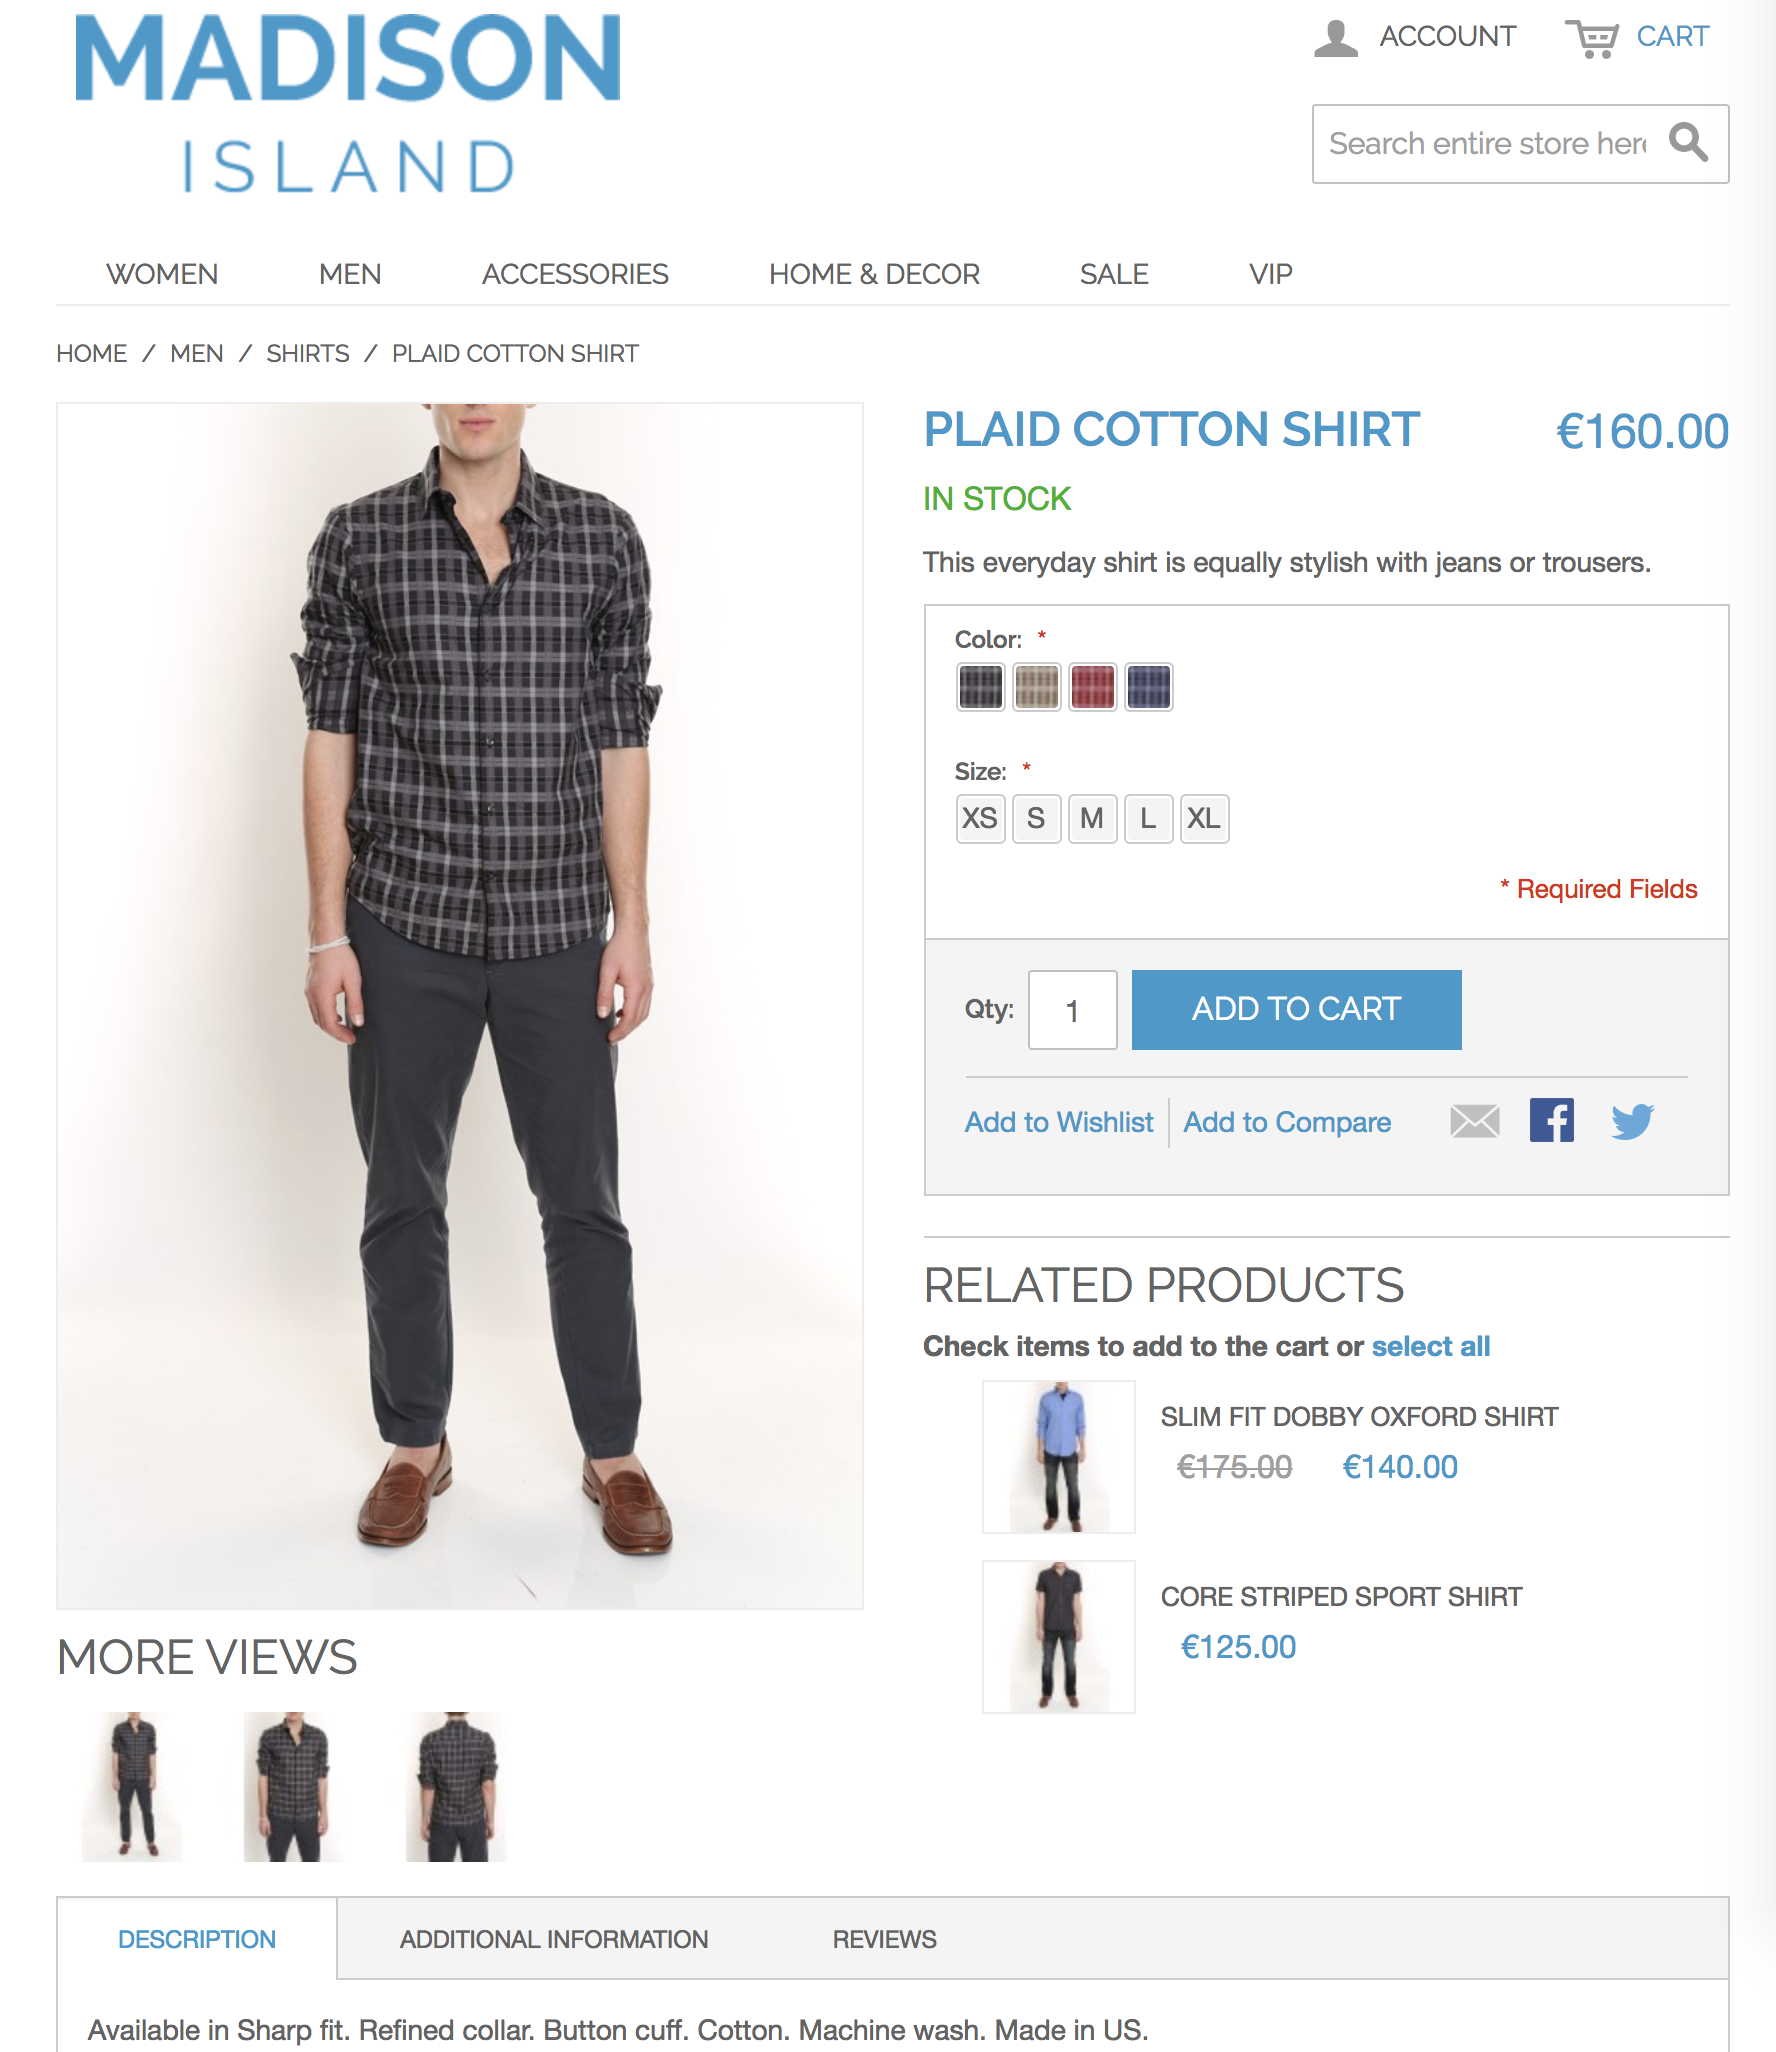
\includegraphics[height=8cm]{images/madison/product-detail.png}
  \caption{Product detail page}
  \label{fig:product-detail}
\end{figure}
\vspace{0.5cm}

The end-to-end interaction from the homepage to the product detail page can be represented by a model using the following IFML notation:

\vspace{0.5cm}
\begin{figure}[H]
  \centering
    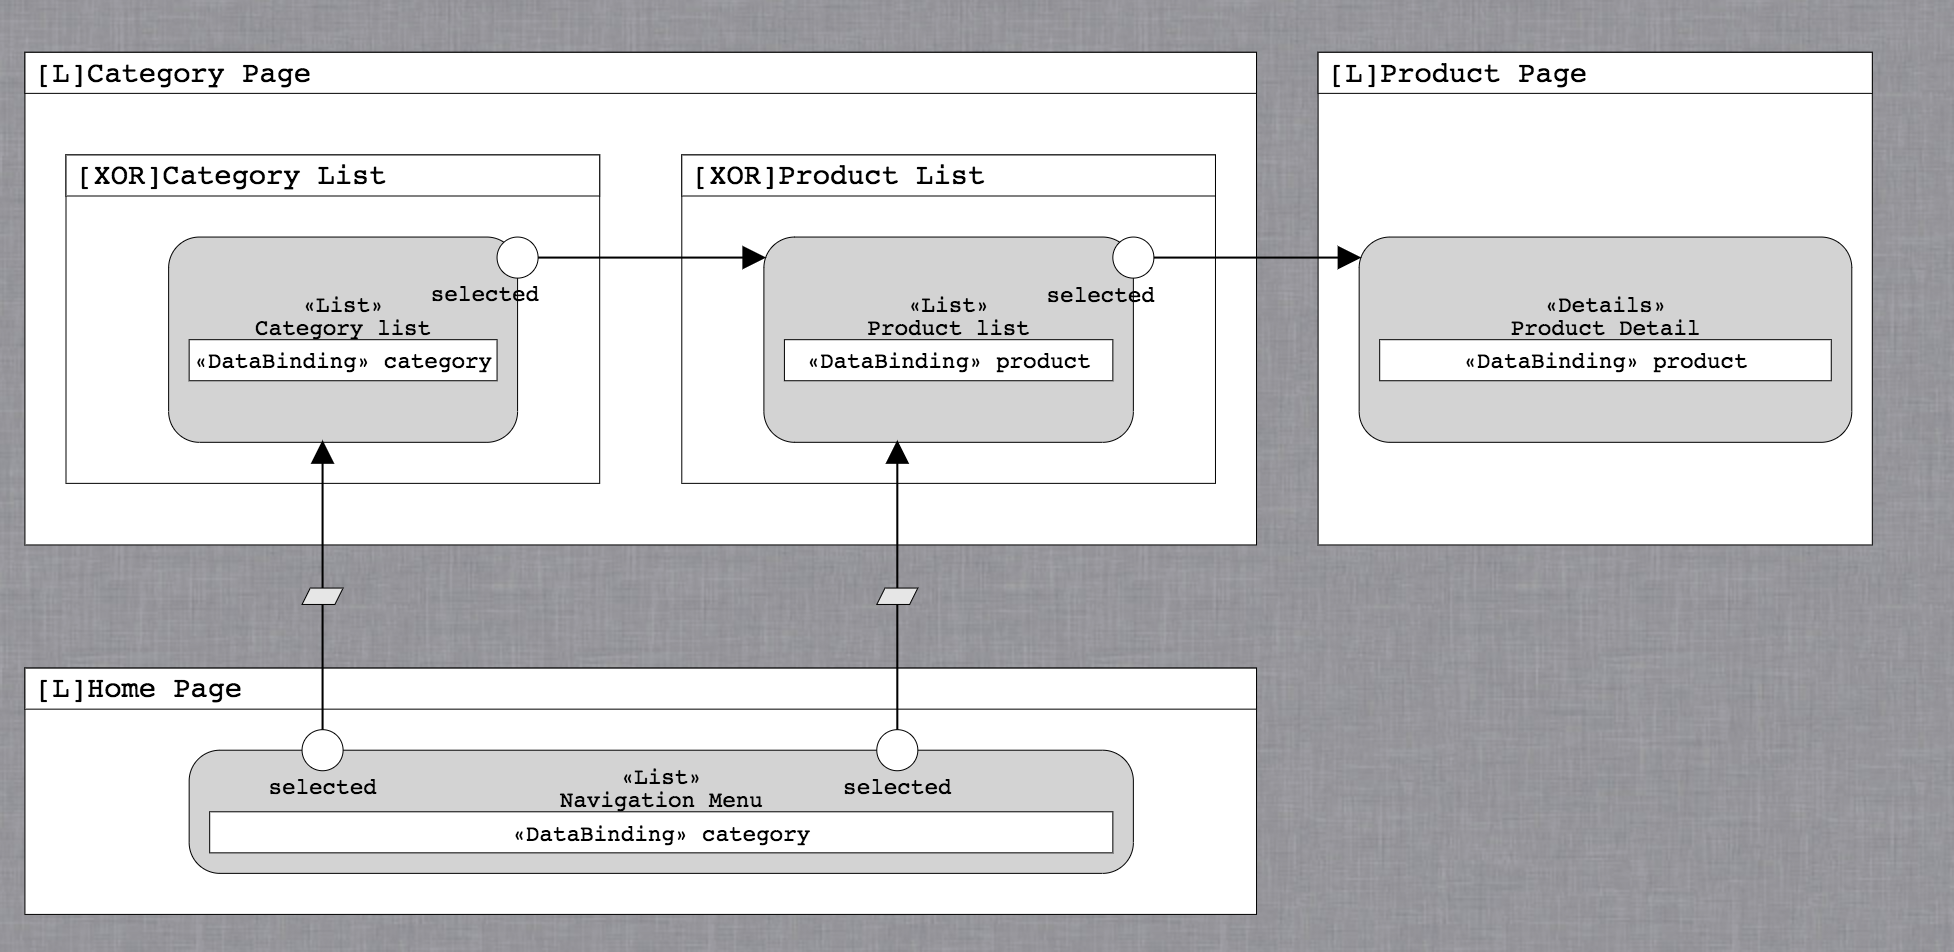
\includegraphics[width=12cm]{images/madison/ifml1.png}
  \caption{IFML representation of the Product Detail interaction}
  \label{fig:ifml1}
\end{figure}
\vspace{0.5cm}

The same sequence of actions can be expressed as a stream of records in the access logs on the application server. Such logs track all the requests processed by the web platform. The following table presents how the above mentioned user journey is logged on the server:

\vspace{0.5cm}
\begin{center}
  \begin{tabular}{|c|p{3cm}|p{10cm}|}
  \hline
  \multicolumn{3}{|c|}{Application Server Access Log}\\ \hline
  \textbf{ID}&\textbf{Page}&\textbf{Log Entry}   \\ \hline
  1&Home Page&\em[29/Nov/2017:06:30:45 +0000] ``GET /" 200 0 - 29505 \\ \hline
  2&\textit{``View All Men"} Category Page &\em[29/Nov/2017:06:49:38 +0000] ``GET /men.html /" 200 0 - 29505 
  \\ \hline
  3&\textit{``Shirts"} Category Page &\em[29/Nov/2017:07:04:15 +0000] ``GET /men/shirts.html" 200 0 - 29505
  \\ \hline
  4&\textit{``Plaid Cotton Shirt"} Product Page &\em[29/Nov/2017:07:08:40 +0000] ``GET /men/shirts/plaid-cotton-shirt-476.html" 200 0 - 29505
  \\ \hline
  \end{tabular}
  \end{center}
  \vspace{0.5cm}

  It is important to notice that both entries 2 and 3 record a \textit{``Category Page"} pageview action by logging their related URLs. The entry 4, on its turn, tracks a \textit{``Product Page"} visit that happened after visiting a category page, logging a specific URL that concatenates the product URL key and the category path. 


\subsection{Products association and correlation}

In this section, we analyse the set of actions that can generate pageviews among different product pages on the Madison Island website. 

For doing so, we consider a \textit{``Related Products"} widget presented to customers just below the \textit{``Add to Cart"} button on the \textit{``Plaid Cotton Shirt"} page discussed on \ref{the-product-page-journey}.

\vspace{0.5cm}
\begin{figure}[H]
  \centering
    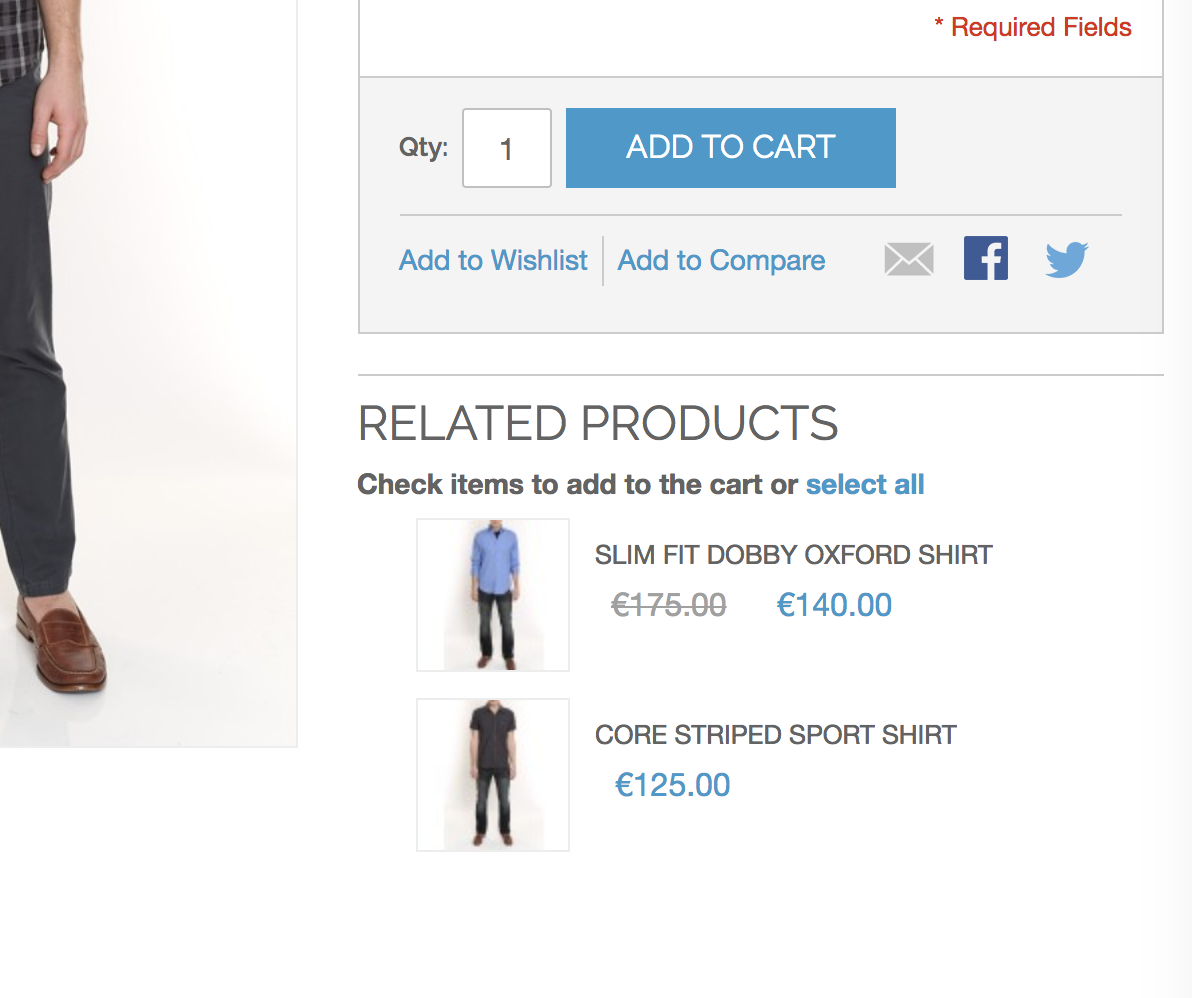
\includegraphics[width=8cm]{images/madison/related-products.png}
  \caption{Related products section}
  \label{fig:related-products}
\end{figure}
\vspace{0.5cm}

By clicking either on the product name or on its thumbnail, the user is directed to the related product page. In this case, we simulate an interest on the listed \textit{``Core Striped Sport Shirt"} (Figure \ref{fig:product-detail2}).

\vspace{0.5cm}
\begin{figure}[H]
  \centering
    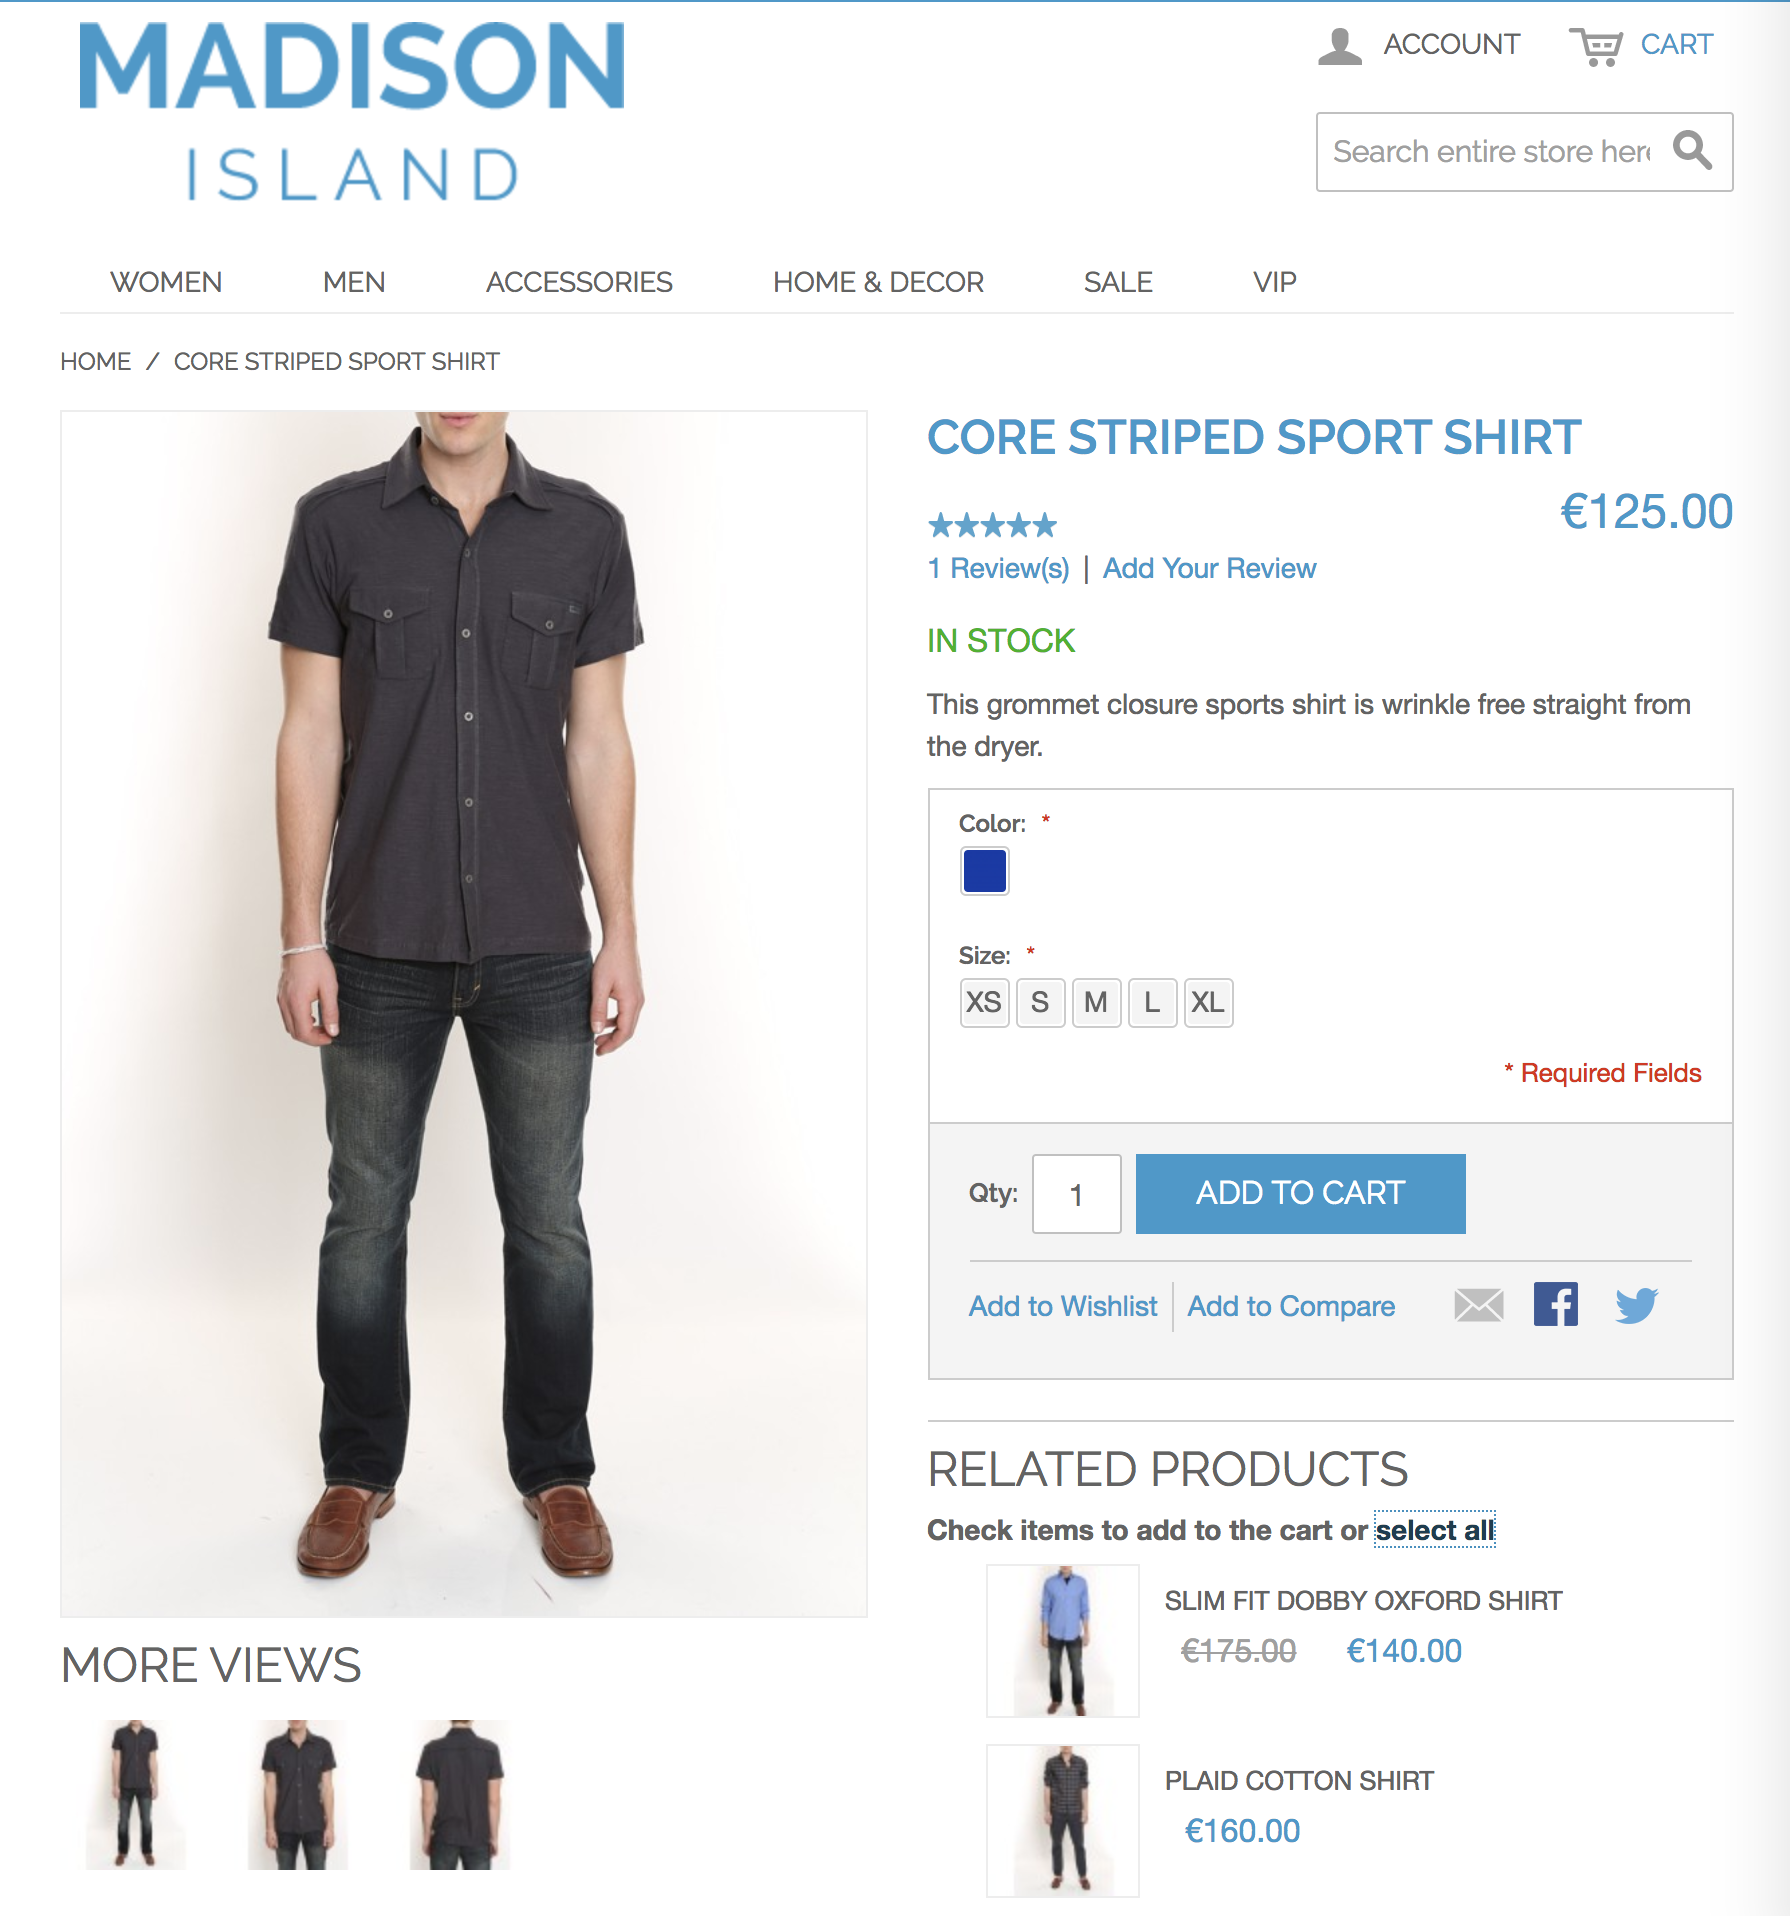
\includegraphics[height=8cm]{images/madison/product-detail2.png}
  \caption{A related product page}
  \label{fig:product-detail2}
\end{figure}
\vspace{0.5cm}

Besides using the simple navigational shortcut available on the related products section, the user can reach a product page in several other ways. For instance, users can click on the ``back" button in their browser to quickly go to the previous category page and to choose a different item. They can also reach the navigation menu to browse another category, or use the search function on the top bar to perform a global product search.
Consequently, the tracking of all these possible user interactions can help in establishing a correlation pattern among different products on the website. Figure \ref{fig:product-search} illustrates the result of the search by the term ``blazer" on the search bar within a given product page.

\vspace{0.5cm}
\begin{figure}[H]
  \centering
    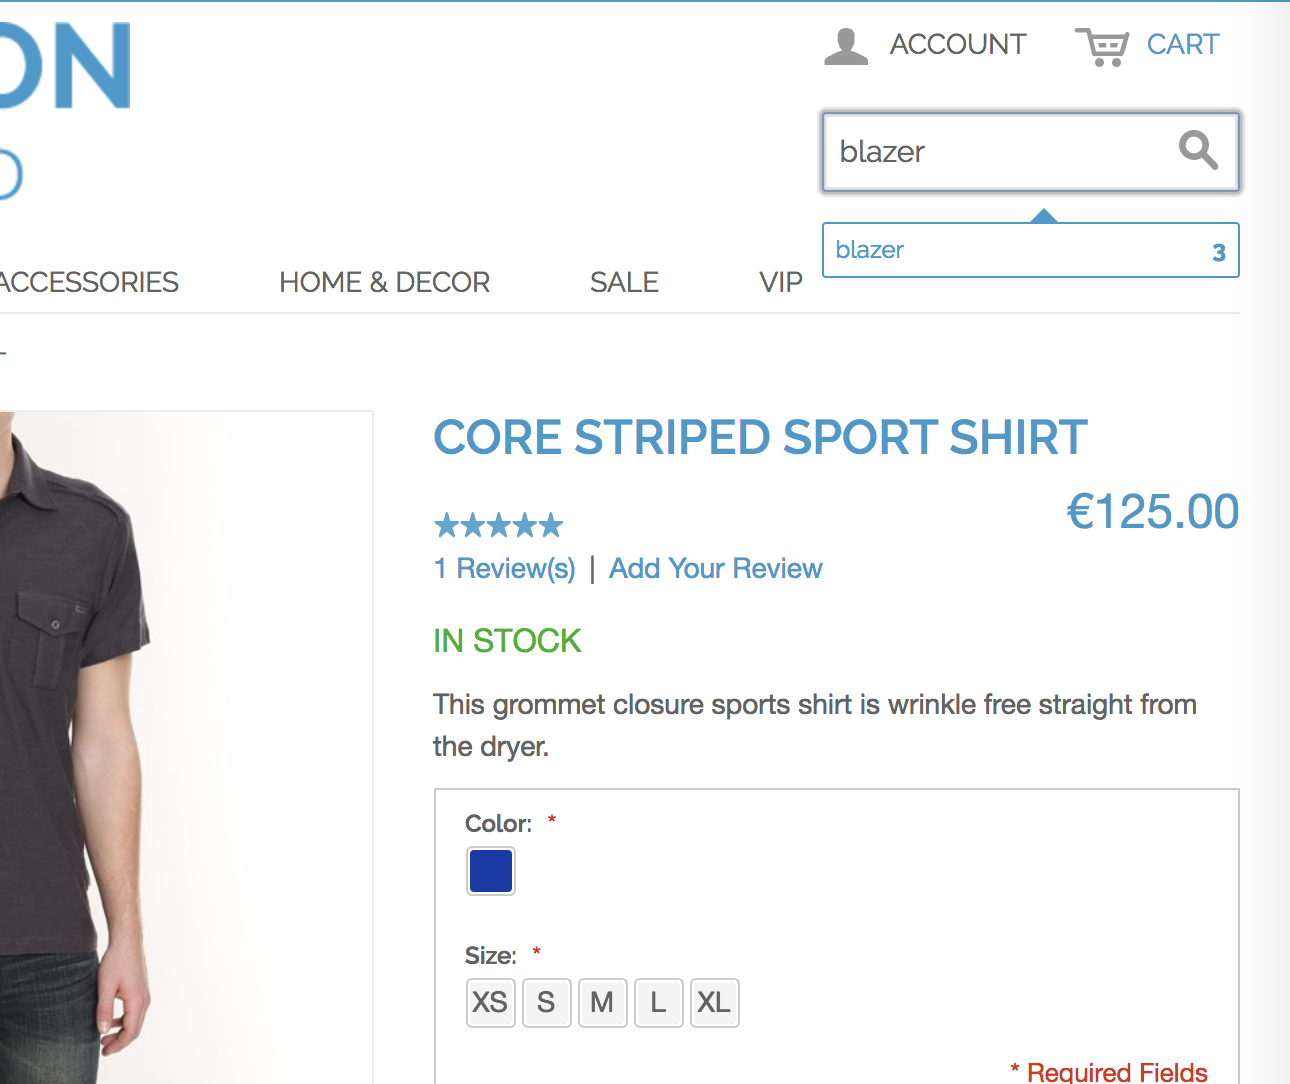
\includegraphics[height=7cm]{images/madison/search.png}
  \caption{Product search bar}
  \label{fig:product-search}
\end{figure}
\vspace{0.5cm}

When the search is performed, the user is taken to the search result page, which lists the products matching the searched term. From there, the user can freely browse to any of the available product pages, similarly to the navigation process described for the category listing page (Figure \ref{fig:search-results}).

\vspace{0.5cm}
\begin{figure}[H]
  \centering
    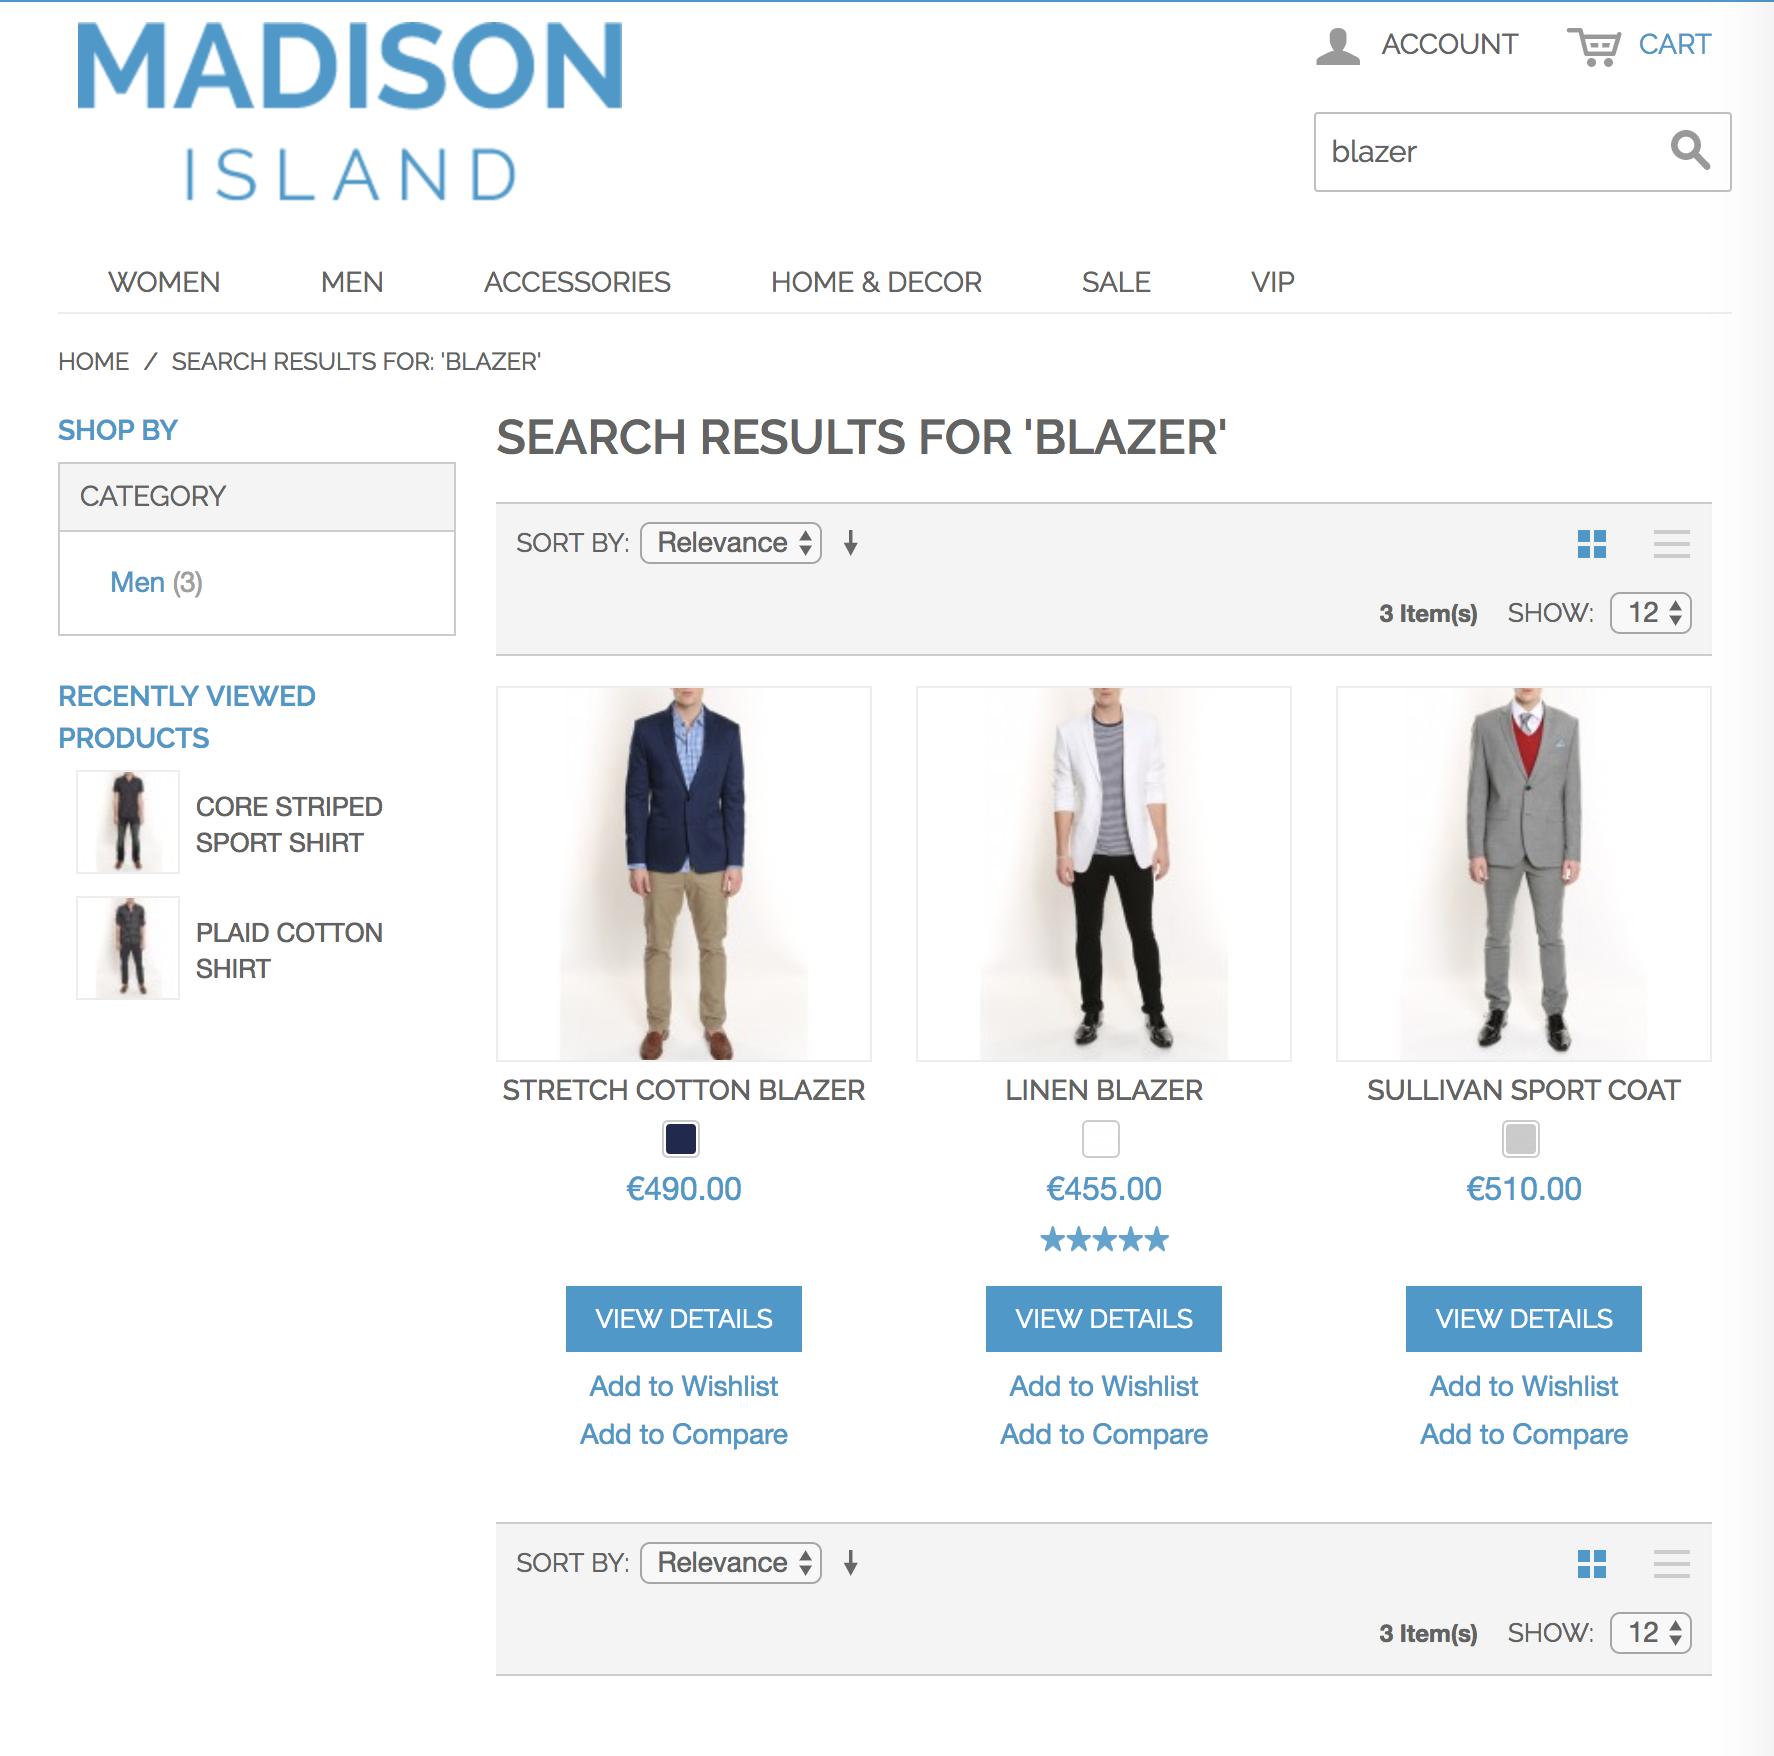
\includegraphics[height=8cm]{images/madison/search-results.png}
  \caption{Search results page}
  \label{fig:search-results}
\end{figure}
\vspace{0.5cm}

At this point, we can update and extend the IFML model shown in Figure \ref{fig:ifml1} according to the new notions and interactions that have been described so far.

\vspace{0.5cm}
\begin{figure}[H]
  \centering
    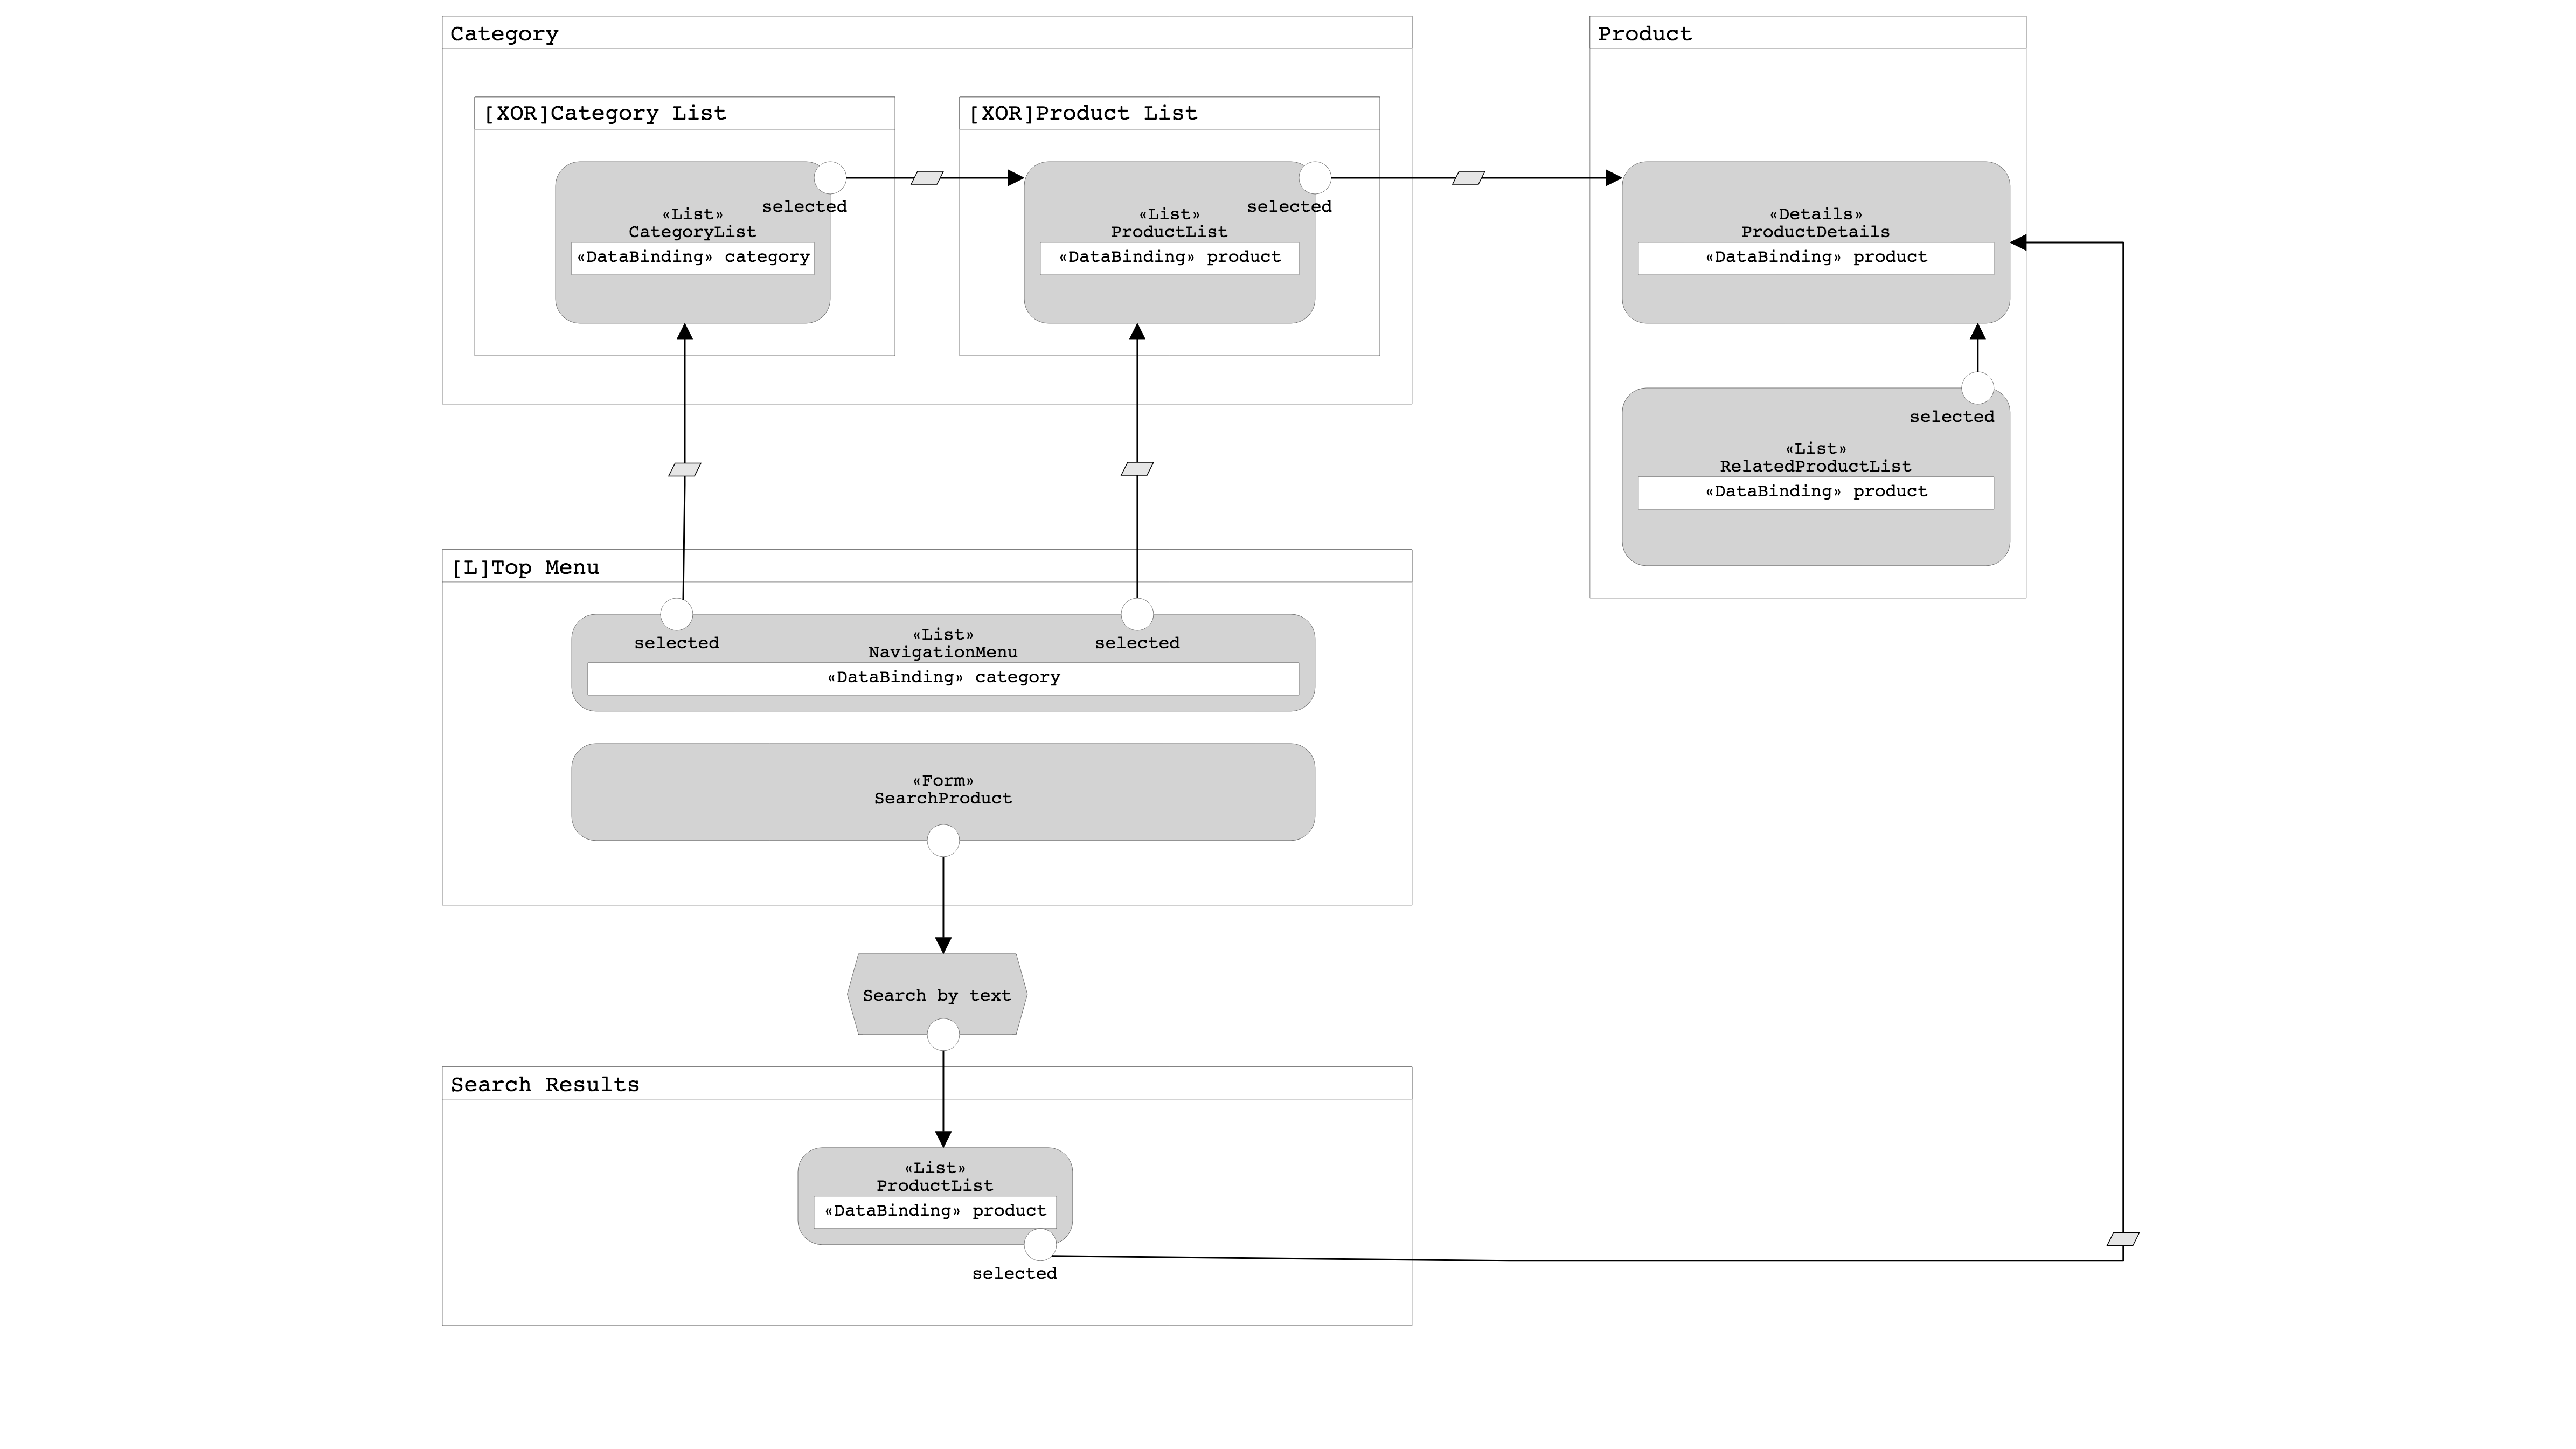
\includegraphics[width=14cm]{images/madison/ifml2.png}
  \caption{Updated IFML representation of the navigational behaviours}
  \label{fig:ifml2}
\end{figure}
\vspace{0.5cm}

These new navigational paths are represented in the application server access log in the following manner: 

\vspace{0.5cm}
\begin{center}
  \begin{tabular}{|c|p{3cm}|p{10cm}|}
  \hline
  \multicolumn{3}{|c|}{Application Server Access Log}\\ \hline
  \textbf{ID}&\textbf{Page}&\textbf{Log Entry}   \\ \hline
  1&\textit{``Plaid Cotton Shirt"} Product Page&\em[04/Dec/2017:06:37:06 +0000] 
  ``GET /men/shirts/plaid-cotton-shirt-476.html" 200 0 - 29505
  \\ \hline
  2&\textit{``Core Striped Sport Shirt"} Product Page &\em [04/Dec/2017:06:37:15 +0000] ``GET /core-striped-sport-shirt-551.html" 200 0 - 29505
  \\ \hline
  3&\textit{``Plaid Cotton Shirt"} Product Page &\em[04/Dec/2017:06:37:21 +0000] ``GET /men/shirts/plaid-cotton-shirt-476.html" 200 0 - 29505
  \\ \hline
  5&\textit{``Tees Knits And Polos"} Category Page &\em[04/Dec/2017:06:38:06 +0000] ``GET /men/tees-knits-and-polos.html" 200 0 - 29505
  \\ \hline
  6&\textit{``Blazer"} Search By Term&\em[04/Dec/2017:06:38:20 +0000] ``GET /catalogsearch/result/?q=blazer" 200 0 - 29505
  \\ \hline
  7&\textit{``Stretch Cotton Blazer"} Product Page &\em[04/Dec/2017:06:38:43 +0000] ``GET /stretch-cotton-blazer-587.html" 200 0 - 29505
  \\ \hline
  \end{tabular}
  \end{center}
\vspace{0.5cm}

The sequence of actions as seen in this log reveals that the user browsed from one product to another, taking advantage of the related product links (ID 2). In fact, the target URL does not include any category path beside the URL key related to the product, which indicates a direct access. The entries 3 and 4 illustrate the journey of an user who has clicked on the browser back button and has performed the same actions again. The last three recorded actions show, respectively, a direct access to a category page through the navigational menu, a search by the \textit{``blazer"} term as per the previous example, and the related redirection to the product page.

\newpage
\section{IoT behaviour profiling}

As mobile devices surpass desktop computers in driving purchases and in enriching behaviour data, location and proximity tracking becomes a valuable tool for brands and stores. In the following subsections, we analyse two possible scenarios of customer interaction in the physical world based on the recording and reporting capabilities of IoT devices. Such data would then be collected together with other web-based information (\ref{beacons}) to form a comprehensive behavioural data stream that could leverage for generating tailored customisations of the Madison eCommerce portal.

\subsection{Apple iBeacon technology and Estimote Beacons overview}

The IoT device chosen to illustrate the scenarios related to the behavioural modeling would be the Estimote Beacons, which use Apple iBeacon technology and are compatible with iBeacon-enabled Apple products and applications.

The company from Cupertino jumped first on the beacon bandwagon by publishing in 2013 a detailed specification (IDs, transmission intervals, etc.) for developing the iBeacon protocol, which in turn allowed vendors, such as Estimote, to ship iBeacon-compatible hardware transmitters worldwide.

\vspace{0.5cm}
\begin{figure}[H]
  \centering
    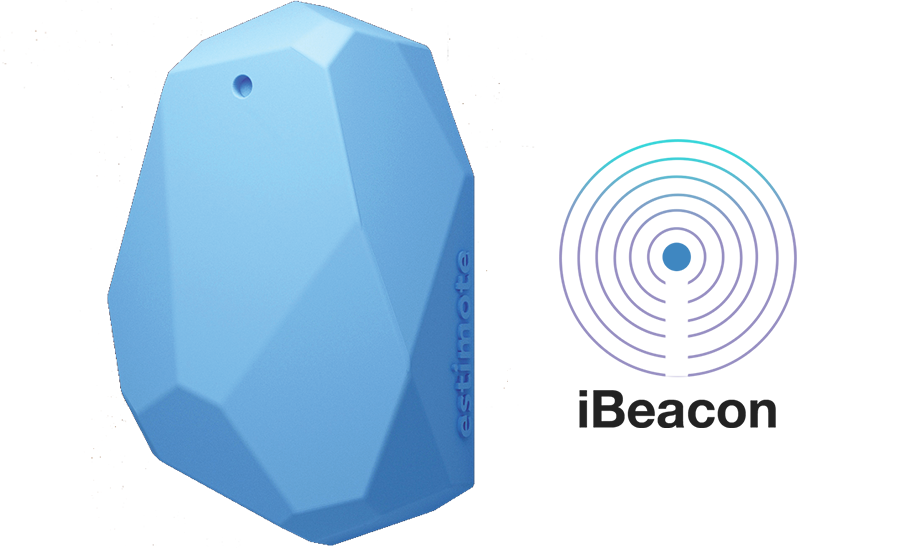
\includegraphics[width=16cm]{images/ibeacon.png}
  \caption{An Estimote iBeacon compatible device}
  \label{fig:estimote-beacon}
\end{figure}
\vspace{0.5cm}

As described in Section \ref{beacons}, a beacon can simply be seen as a lighthouse that broadcasts information in certain intervals and at a defined power, leveraging Low Energy Bluetooth connection. In the case of iBeacons, the information sent to listening mobile devices would contain:


\begin{itemize}
  \item The Universal Unique ID (UUID), which is globally unique. Example: de2b45ae-ed98-11e4-3432-78616d6f6f6d
  \item The Major ID, which uniquely identifies our customer’s system: e.g. 51314
  \item The Minor ID, which reports the exact location or object (in our case, the spot): e.g. 23369
\end{itemize}

Unlike QR and NFC communication, the customer needs to have an app installed on their phone to receive this one-way data stream. Technically, the app obeys only to iBeacons with UUID, Major and Minor IDs matching to predefined values. When that happens, the app can react accordingly. Such mechanism ensures that only the installed app can track users as they walk around the transmitters. 

In other words, the phone OS will keep listening for beacons even if the app is not running, and even if the phone is locked or rebooted. Once either an “enter” or and “exit” event happens, the OS will launch the app into the background (if needed) and let it execute, for a few seconds, some code to handle the event.

\subsection{Proximity Marketing}
\label{section:proximity-marketing}

Proximity Marketing is an efficient tool not only for discovering and engaging new customers, but also for better targeting existing ones. This marketing technique operates in a given physical location by leveraging the IoT ecosystem to promote products and services.  This communication channel acts on a clear target: all the customers close to, or within, an area covered by the diffusion devices.

Such innovative form of relationship marketing aims to activate and involve users by drawing their attention at the right time and in the right place, creating more intense and stimulating shopping experiences.

In this work, we will focus on a basic scenario where the recognition of proximity in the physical world does not directly trigger an immediate action to grab customer attention, but instead is limited to the silent tracking of the event as well as the automatic recording of data on a specific web server.

We start by defining a possible allocation of items for a ``Madison Island" retail store, which resembles the catalogue presented on its website.

\vspace{0.5cm}
\begin{figure}[H]
  \centering
    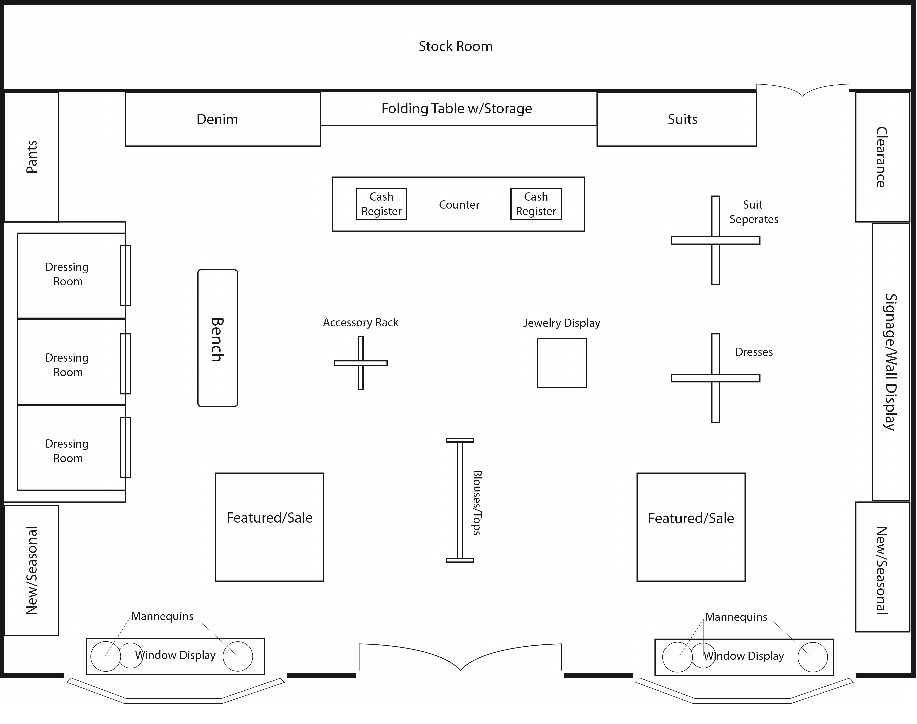
\includegraphics[width=15cm]{images/madison/retail-map.jpg}
  \caption{Madison Island brick-and-mortar store map}
  \label{fig:retail-map}
\end{figure}
\vspace{0.5cm}

Each label described in Figure~\ref{fig:retail-map} represents a specific category of the website, whereas the color of the label indicates the parent category to which the products belong. More specifically:

\begin{itemize}
  \item Red represents the \textbf{Women} category, which maps the content available at \textbf{/women.html}. 
  \item Blue represents the \textbf{Men} category, which maps the content available at \textbf{/men.html}.
  \item Purple represents the \textbf{Home \& Decor} category, which maps the content available at \textbf{/home-decor.html}. 
  \item Orange represents the \textbf{Accessories} category, which maps the content available at \textbf{/accessories.html}. 
\end{itemize}

As a customer walks around the physical shop, the Madison Island mobile app looks for a predefined set of beacon regions. Whenever the device either enters or exits each region, the app registers proximity data and tracks the aisles (regions) visited or not by the customer.

In this scenario, the following image illustrates what would be a suitable Estimote beacon allocation for the store:

\vspace{0.5cm}
\begin{figure}[H]
  \centering
    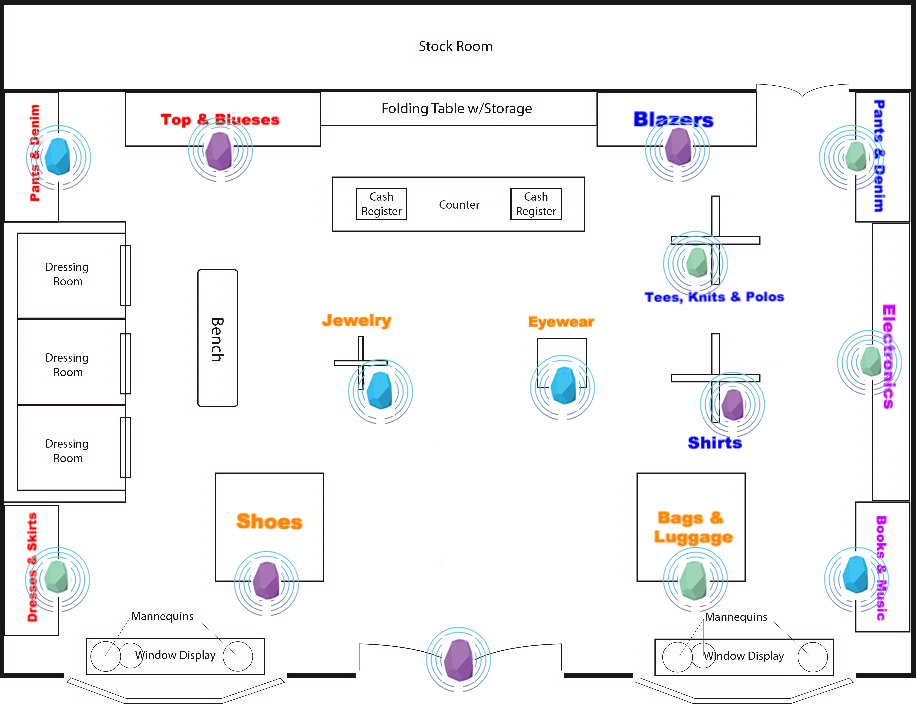
\includegraphics[width=14cm]{images/madison/retail-map-beacon.jpg}
  \caption{Madison Island brick-and-mortar store with Estimote beacons allocation}
  \label{fig:beacons-map}
\end{figure}
\vspace{0.5cm}

Depending on the business use case, the mobile app can either send an event to the listening server whenever the user crosses a region boundary, or submit a single event with a full list of regions and their minimum proximities detected during the customer visit. 

Due to the behavioural profiling nature of this activity, we assume that the app does the latter, detecting all the entering and leaving of each virtual fence and activating a \textit{ranging} procedure that detects proximity information based on the strength of the Bluetooth signal.\cite{region-monitoring-apple}.

Once the shoppers leaves the physical store, the app performs a single data push to a REST API endpoint with all the tracked data.

From a technical perspective, all these operations are accomplished leveraging the Estimote iOS-SDK\cite{estimote-ios-sdk}, which allows the developer to quickly define regions and ranges for each beacon and facilitates the tracking of the actual proximity to beacon through the ranging process.

As an example, the JSON payload sent from the app to the REST endpoint for an hypothetical customer 3045678 (e.g. \textbf{POST /users/3045678/sessions}) would have the following structure:


\vspace{0.5cm}
\begin{lstlisting}[language=json,firstnumber=1]
  {
    ``data":{
       ``customerId":3045678,
       ``storeId":8784,
       ``storeLabel" : ``Madison1",
       ``sessionId" : ``89376f84-065b-11e8-ba89-0ed5f89f718b"

       ``sessionRegions":[
             {
                "regionId: : 156,
                ``regionLabel":``store-entrance",
                ``detectionCount":2,
                ``maxSecondsInRegion": 5,
                ``maxProximity":``unknown",
                ``firstDetectionTimestamp":"2018-02-21T18:09:07Z",
                ``lastDetectionTimestamp":"2018-02-21T18:16:02Z",
                ``beaconData" : {
                  ``uuid":``0686a88e-fed6-11e7-8be5-0ed5f89f718b",
                  ``majorId":2553,
                  ``minorId":79
                }
             },
             {
                "regionId: : 645,
                ``regionLabel":``shoes",
                ``detectionCount":1,
                ``maxSecondsInRegion": 24,
                ``maxProximity":``near",
                ``firstDetectionTimestamp":"2018-02-21T18:09:20Z",
                ``lastDetectionTimestamp":"2018-02-21T18:09:20Z",
                ``beaconData" : {
                  ``uuid":``0686a88e-fed6-11e7-8be5-0ed5f89f718b",
                  ``majorId":19029,
                  ``minorId":49
                }
             },
             {
                ``regionId" : 6875,
                ``regionLabel":``jewelry",
                ``detectionCount":1,
                ``maxSecondsInRegion": 15,
                ``maxProximity":``far",
                ``firstDetectionTimestamp":"2018-02-21T18:10:15Z",
                ``lastDetectionTimestamp":"2018-02-21T18:10:15Z",
                ``beaconData" : {
                  ``uuid":``0686a88e-fed6-11e7-8be5-0ed5f89f718b",
                  ``majorId":38415,
                  ``minorId":59
                }
             },
             {
                ``regionId" : 2563,
                ``regionLabel":``blazers",
                ``detectionCount":1,
                ``maxSecondsInRegion": 195,
                ``maxProximity":``immediate",
                ``firstDetectionTimestamp":"2018-02-21T18:11:01Z",
                ``lastDetectionTimestamp":"2018-02-21T18:11:01Z",
                ``beaconData" : {
                  ``uuid":``0686a88e-fed6-11e7-8be5-0ed5f89f718b",
                  ``majorId":25911,
                  ``minorId":27
                }
             },
             {
                ``regionId" : 456,
                ``regionLabel":``tees-knits-polos",
                ``detectionCount":1,
                ``maxSecondsInRegion": 10,
                ``maxProximity":``far",
                ``firstDetectionTimestamp":"2018-02-21T18:14:56Z",
                ``lastDetectionTimestamp":"2018-02-21T18:14:56Z",
                ``beaconData" : {
                  ``uuid":``0686a88e-fed6-11e7-8be5-0ed5f89f718b",
                  ``majorId":42037,
                  ``minorId":36
                }
             },
             {
                ``regionId" : 998,
                ``regionLabel":``bags-and-luggage",
                ``detectionCount":1,
                ``maxSecondsInRegion": 7,
                ``maxProximity":``far",
                ``firstDetectionTimestamp":"2018-02-21T18:15:12Z",
                ``lastDetectionTimestamp":"2018-02-21T18:15:12Z",
                ``beaconData" : {
                  ``uuid":``0686a88e-fed6-11e7-8be5-0ed5f89f718b",
                  ``majorId":37931,
                  ``minorId": 85
                }
             }
          ]
    }
 }
  \end{lstlisting}
\vspace{0.5cm}


The above example session shows an evident preference for ``Blazer" items, and a slight interest in ``Shoes" items. More precisely, the ``Blazer" region registered a session that lasted over 3 minutes and that was the closest to a beacon.  

\subsection{Customer Rewards}

Besides allowing proximity based marketing, beacon technology can also be used to reward customers for particular actions based on geolocalisation data. Such rewards could increase brand engagement, enhancing customer loyalty and fostering lasting customer relationships. 

Achieving such results is possible by extending the set of actions that enable customers to earn bonuses and discounts on the website (newsletter subscriptions, minimum order amount, etc..) to activities performed in the physical world, including the simple act of visiting and walking around the brick-and-mortar store.

For example, the brand can rank customers by the amount of time spent at each Madison Retail shop, rewarding them with monthly offers tailored according to their purchases. The brand can also focus on offering special offers on the website to the customers that visited a retail store in a specific time span, such as Christmas.

For our Madison Island example, we are considering a scenario where customers are rewarded with a fixed amount of points on their online account if they scan three QR codes from in-store products. Specifically, when the beacon detects their entrance into the store, the mobile app pushes a CheckPoints notification to the customer, inviting them to scan codes of items available in the shop. Once the scans are correctly performed within a session, the mobile app pushes the information to the same REST API presented in the previous chapter, which then stores the data.

\vspace{0.5cm}
\begin{figure}[H]
  \centering
    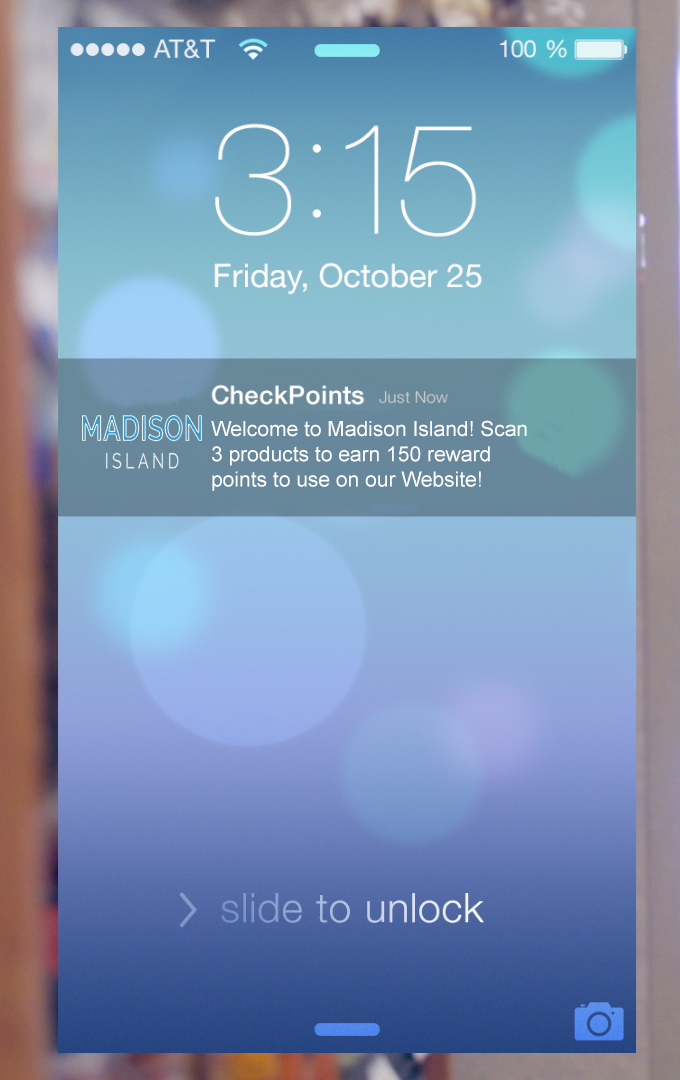
\includegraphics[width=8cm]{images/madison-push-reward-points.jpg}
  \caption{Madison Island mobile app push notification example}
  \label{fig:mobile-app-push-notification}
\end{figure}
\vspace{0.5cm}


The JSON payload sent to the server (e.g. \textbf{POST /users/3045678/scans}) after each successful scan would then have a structure similar to the following one:
 
\vspace{0.5cm}
\begin{lstlisting}[language=json,firstnumber=1]
  {
    ``data":{
       ``customerId":3045678,
       ``storeId":8784,
       ``storeLabel" : ``Madison1",
       ``sessionId" : ``89376f84-065b-11e8-ba89-0ed5f89f718b"
       ``sessionDuration" : 456,
       ``sessionActions": [{
          ``userAgent" : ``Iphone 6s",
          ``scannedItems":
            [{
              ``barcode":``042100005264",
              ``name" : ``Elizabeth Knit Top-Red-S"
              ``sku": ``wbk012c-Red-S"    
            },
            {
              ``barcode":``042100005931",
              ``name" : ``Plaid Cotton Shirt-Khaki-L"
              ``sku": ``msj006c-Khaki-L"    
            },
            {
              ``barcode":``042100007717",
              ``name" : ``Broad St Saddle Shoes"
              ``sku": ``shm00110"    
            }
            ]
      }]
    }
 }
  \end{lstlisting}
\vspace{0.5cm}


Similarly to the process outlined in \ref{section:proximity-marketing}, the product data collected when customers scan codes during their visits to the physical store will potentially be converted into reward points to be used by the same customer on the website.  


\clearpage

 % !TEX root = Tesi.tex
\chead{}
\chapter{Our approach to modeling}

While in the last chapter we introduced three different streams of real usage data obtained both from the physical and the virtual world, we now focus on expanding those representations in a more detailed way with the help of the Model-Driven Engineering techniques briefly described in \ref{model-driven-techniques}. 
Concretely, the goal of the first two sections is to illustrate the defining languages (metamodels) for both the real usage data and the eCommerce platform interactions described in the previous examples. Besides, we will generate actual models based upon those metamodels, which represent the very same information.
Finally, in the last section, we will use the same model generation for updating the models instantiated previously, leveraging model transformation techniques based upon usage pattern detection resulting from the Big Data analysis.

\section{Real usage data modeling}

\subsection{Metamodel}

The representation of the real usage data starts from the definition of the metamodel that defines the languages and processes from which to form a model without making statements about its content. In fact, a metamodel is itself a model that is used to describe another model by using a modeling language at a different level of abstraction.  

Figure in \ref{fig:real-usage-data-metamodel-diagram} describes the processed metamodel as a UML Class Diagram according to the data retrieved for our real usage data analysis.

\vspace{0.5cm}
\begin{figure}[H]
  \centering
    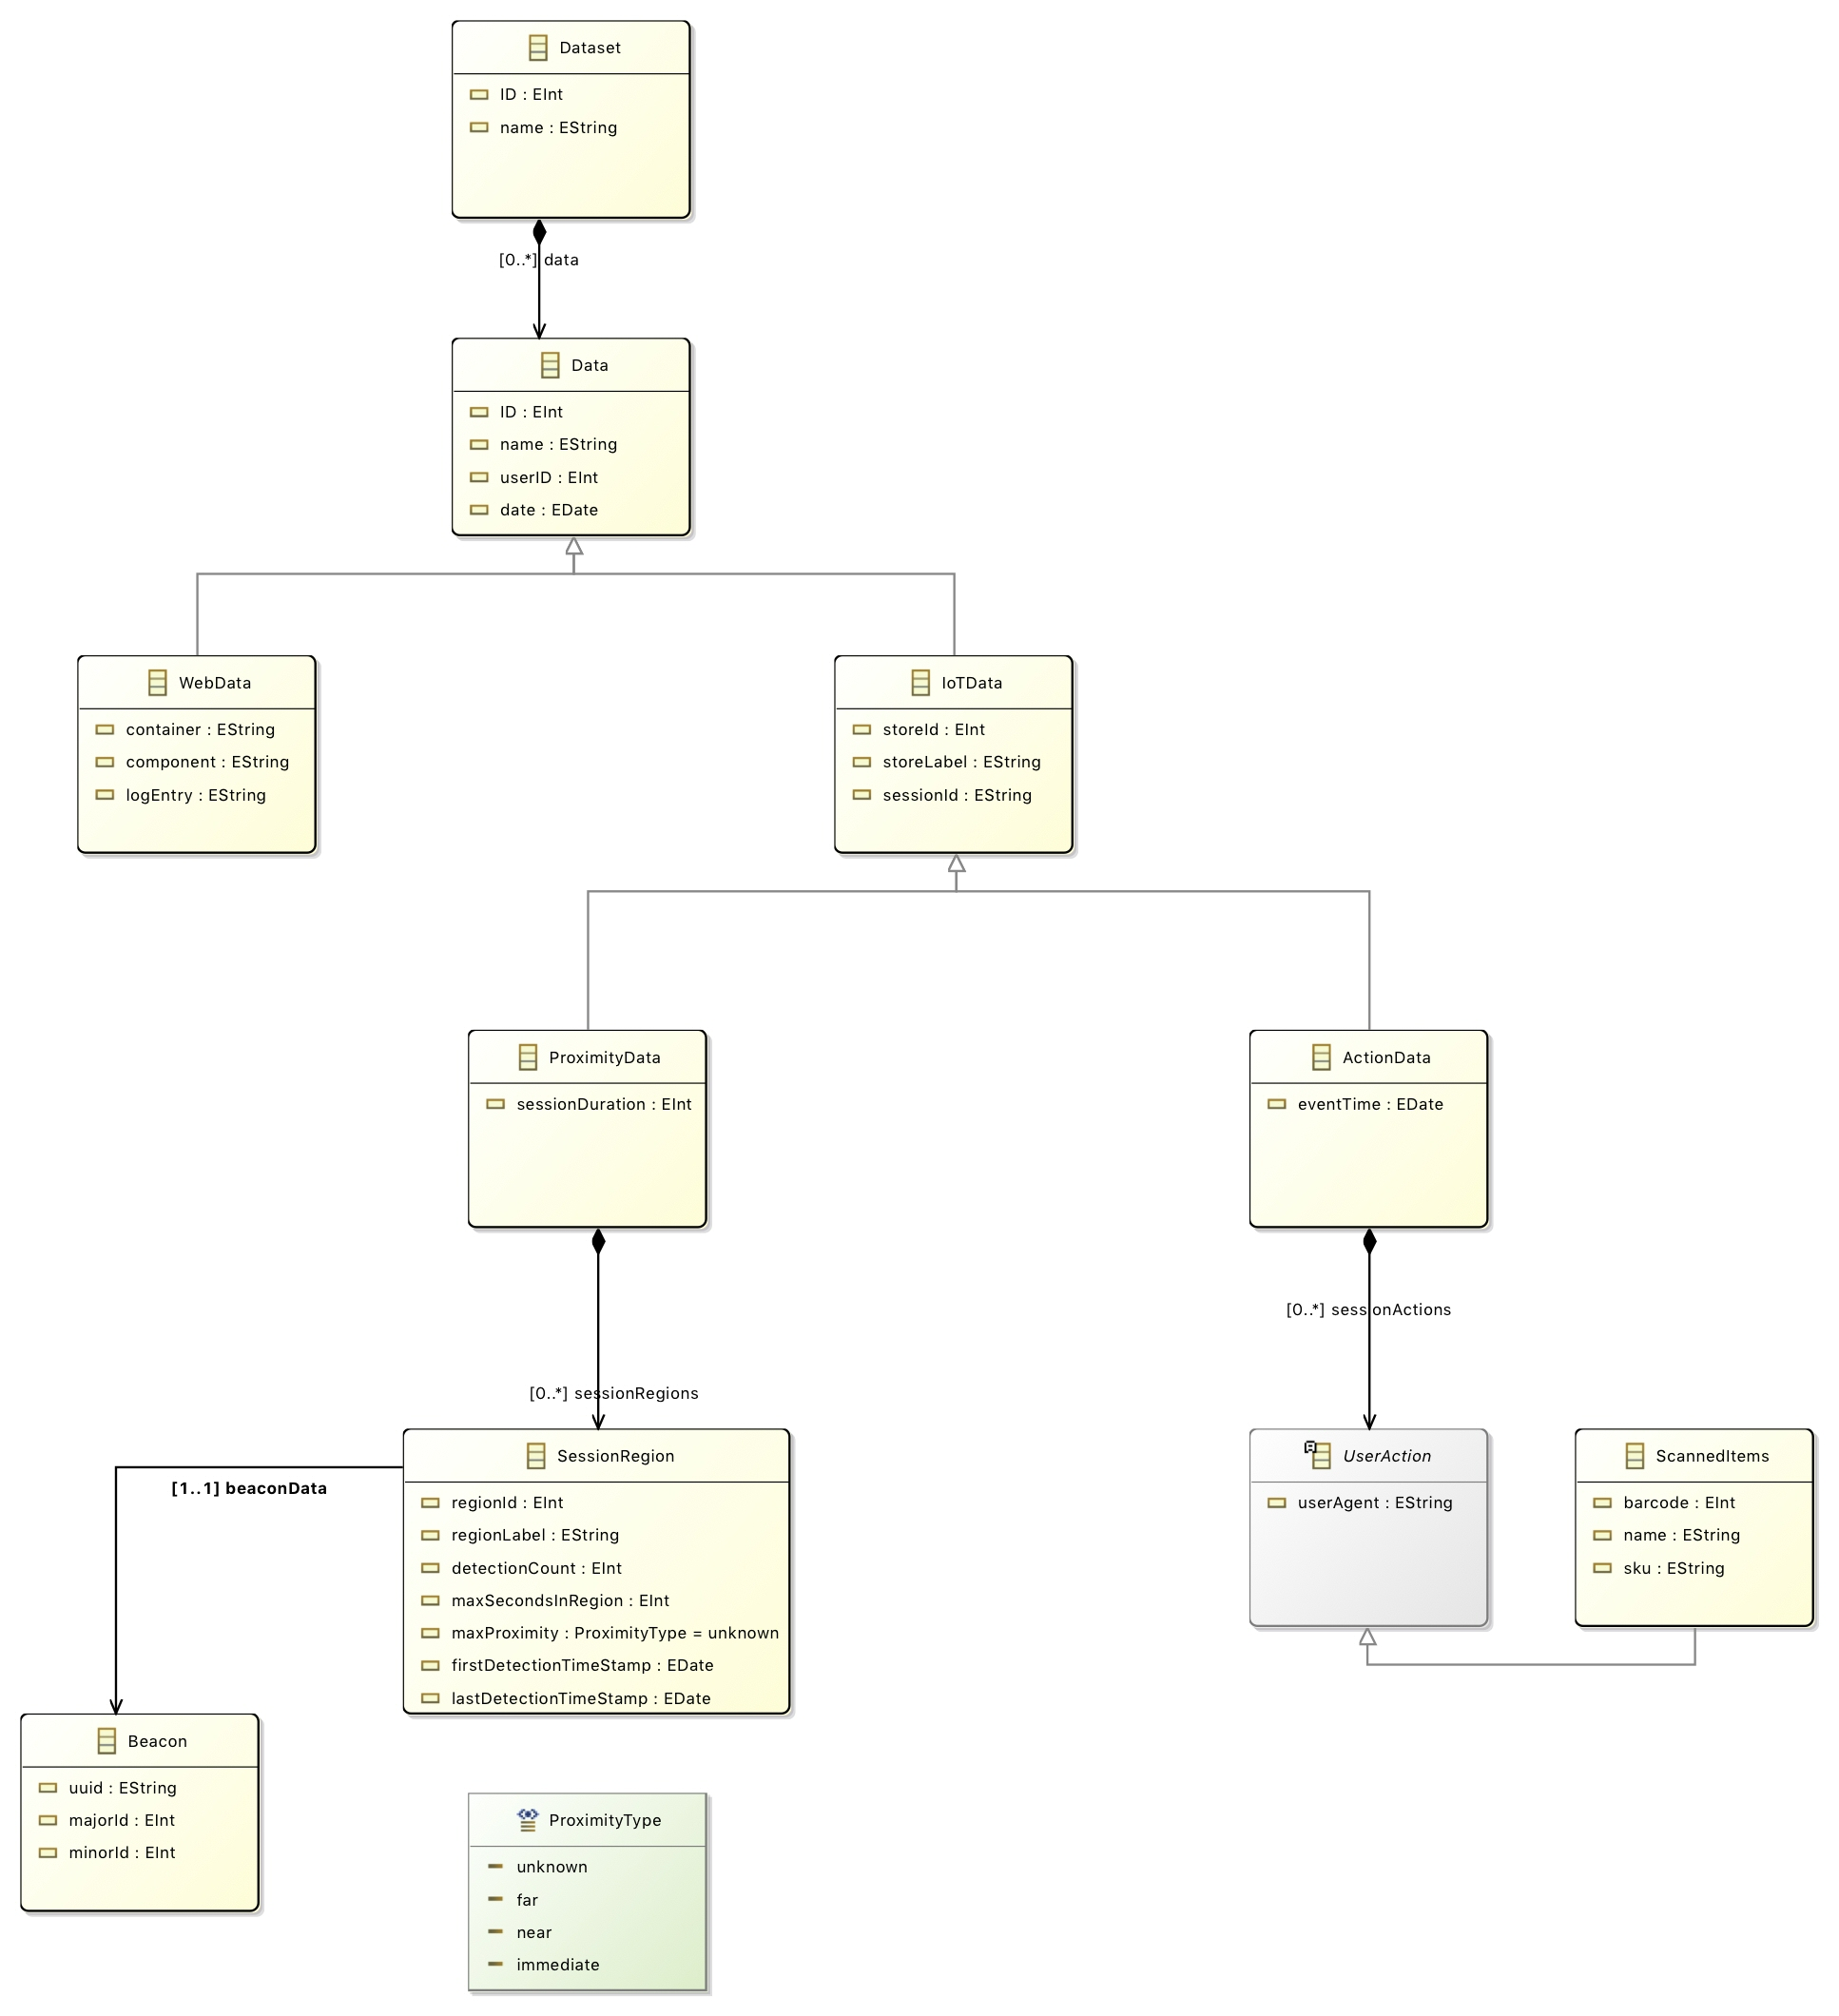
\includegraphics[height=19cm]{images/diagrams/RealUsageDataMetamodel.jpg}
  \caption{Real Usage Data Metamodel Diagram Class}
  \label{fig:real-usage-data-metamodel-diagram}
\end{figure}
\vspace{0.5cm}

\newpage
\subsection{Model}
\label{real-usage-data-model}

The RealUsageData metamodel defined above allows us to create dynamic instances that precisely map the real usage data collected both from web mining process and from IoT devices tracking. Figure \ref{fig:real-usage-data-model} illustrates this processed model in its ecore representation form in Eclipse Modeling Tools (EMF). The figure is followed by the corresponding XMI file content.

\vspace{0.5cm}
\begin{figure}[H]
  \centering
    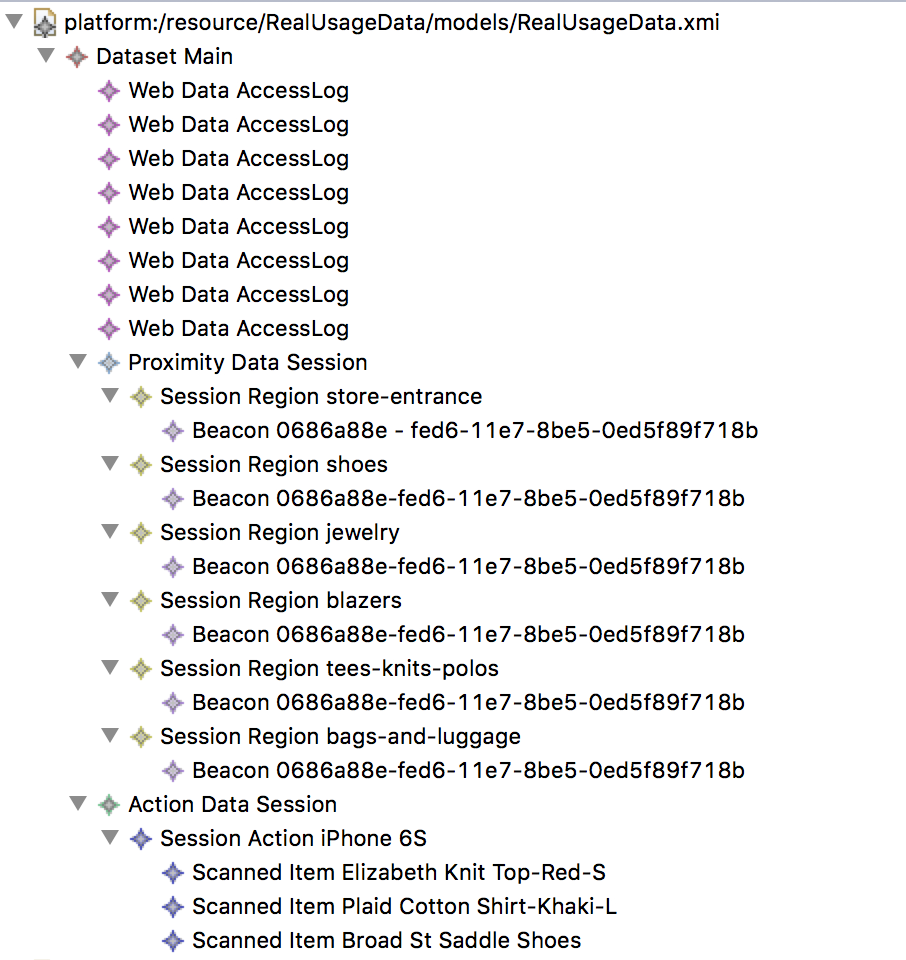
\includegraphics[height=12cm]{images/diagrams/RealUsageDataModel.png}
  \caption{Real Usage Data Model in EMF}
  \label{fig:real-usage-data-model}
\end{figure}
\vspace{0.5cm}

\lstset{language=XML}
\begin{lstlisting} 
<?xml version="1.0" encoding="UTF-8"?>
<RealUsageData:Dataset
    xmi:version="2.0"
    xmlns:xmi="http://www.omg.org/XMI"
    xmlns:xsi="http://www.w3.org/2001/XMLSchema-instance"
    xmlns:RealUsageData="RealUsageData"
    xsi:schemaLocation="RealUsageData ../metamodels/RealUsageData.ecore"
    ID="1" name="Main">
  <data xsi:type="RealUsageData:WebData"
      ID="1"
      name="AccessLog"
      userID="3045678"
      date="2017-11-29T17:06:49.000+0100"
      viewContainer="Homepage"
      viewComponent="TopMenu"
      eventType="click"
      parameterBindingGroup="Category/5"
      logEntry="GET /men.html / 200 0 - 29505"/>
  <data xsi:type="RealUsageData:WebData"
      ID="2"
      name="AccessLog"
      userID="3045678"
      date="2017-11-29T17:07:04.000+0100"
      viewContainer="Category #5"
      viewComponent="CategoryList"
      eventType="click"
      parameterBindingGroup="Category/15"
      logEntry="GET /men/shirts.html 200 0 - 29505"/>
  <data xsi:type="RealUsageData:WebData"
      ID="3"
      name="AccessLog"
      userID="3045678"
      date="2017-11-29T07:08:40.000+0100"
      viewContainer="Category #15"
      viewComponent="ProductList"
      eventType="click"
      parameterBindingGroup="Product/404"
      logEntry="GET /men/shirts/plaid-cotton-shirt-476.html 200 0 - 29505"/>
  <data xsi:type="RealUsageData:WebData"
      ID="4"
      name="AccessLog"
      userID="3045678"
      date="2017-12-04T06:37:15.000+0100"
      viewContainer="Product #404"
      viewComponent="RelatedProductList"
      eventType="click"
      parameterBindingGroup="Product/413"
      logEntry="GET /core-striped-sport-shirt-551.html 200 0 - 29505"/>
  <data xsi:type="RealUsageData:WebData"
      ID="5"
      name="AccessLog"
      userID="3045678"
      date="2017-12-04T06:37:21.000+0100"
      viewContainer=""
      viewComponent=""
      eventType="backButton"
      parameterBindingGroup=""
      logEntry="GET /men/shirts/plaid-cotton-shirt-476.html 200 0 - 29505"/>
  <data xsi:type="RealUsageData:WebData"
      ID="6"
      name="AccessLog"
      userID="3045678"
      date="2017-12-04T06:38:06.000+0100"
      viewContainer="Product #404"
      viewComponent="TopMenu"
      eventType="click"
      parameterBindingGroup="Category/16"
      logEntry="GET /men/tees-knits-and-polos.html 200 0 - 29505"/>
  <data xsi:type="RealUsageData:WebData"
      ID="7"
      name="AccessLog"
      userID="3045678"
      date="2017-12-04T06:38:20.000+0100"
      viewContainer="Category #16"
      viewComponent="TopSearch"
      eventType="submit"
      parameterBindingGroup="SearchText/blazer"
      logEntry="GET /catalogsearch/result/?q=blazer 200 0 - 29505"/>
  <data xsi:type="RealUsageData:WebData"
      ID="8"
      name="AccessLog"
      userID="3045678"
      date="2017-12-04T06:38:20.000+0100"
      viewContainer="Search Results"
      viewComponent="ProductList"
      eventType="click"
      parameterBindingGroup="Product/407"
      logEntry="GET /stretch-cotton-blazer-587.html 200 0 - 29505"/>
  <data xsi:type="RealUsageData:ProximityData"
      ID="9"
      name="Session"
      userID="3045678"
      date="2018-02-21T18:16:07.000+0100"
      storeId="8784"
      storeLabel="Madison1"
      sessionId="89376f84-065b -11e8- ba89-0ed5f89f718b"
      sessionDuration="345">
    <sessionRegions
        regionId="156"
        regionLabel="store-entrance"
        detectionCount="2"
        maxSecondsInRegion="5"
        firstDetectionTimeStamp="2018-02-21T18:09:07.000+0100"
        lastDetectionTimeStamp="2018-02-21T18:16:02.000+0100">
      <beaconData
          uuid="0686a88e - fed6-11e7-8be5-0ed5f89f718b"
          majorId="2553"
          minorId="79"/>
    </sessionRegions>
    <sessionRegions
        regionId="645"
        regionLabel="shoes"
        detectionCount="1"
        maxSecondsInRegion="24"
        maxProximity="near"
        firstDetectionTimeStamp="2018-02-21T18:09:20.000+0100"
        lastDetectionTimeStamp="2018-02-21T18:09:20.000+0100">
      <beaconData
          uuid="0686a88e-fed6-11e7-8be5-0ed5f89f718b"
          majorId="19029"
          minorId="49"/>
    </sessionRegions>
    <sessionRegions
        regionId="6875"
        regionLabel="jewelry"
        detectionCount="1"
        maxSecondsInRegion="15"
        maxProximity="far"
        firstDetectionTimeStamp="2018-02-21T18:10:15.000+0100"
        lastDetectionTimeStamp="2018-02-21T18:10:15.000+0100">
      <beaconData
          uuid="0686a88e-fed6-11e7-8be5-0ed5f89f718b"
          majorId="38415"
          minorId="59"/>
    </sessionRegions>
    <sessionRegions
        regionId="2563"
        regionLabel="blazers"
        detectionCount="1"
        maxSecondsInRegion="195"
        maxProximity="immediate"
        firstDetectionTimeStamp="2018-02-21T18:11:01.000+0100"
        lastDetectionTimeStamp="2018-02-21T18:11:01.000+0100">
      <beaconData
          uuid="0686a88e-fed6-11e7-8be5-0ed5f89f718b"
          majorId="25911"
          minorId="27"/>
    </sessionRegions>
    <sessionRegions
        regionId="456"
        regionLabel="tees-knits-polos"
        detectionCount="1"
        maxSecondsInRegion="10"
        maxProximity="immediate"
        firstDetectionTimeStamp="2018-02-21T18:14:56.000+0100"
        lastDetectionTimeStamp="2018-02-21T18:14:56.000+0100">
      <beaconData
          uuid="0686a88e-fed6-11e7-8be5-0ed5f89f718b"
          majorId="42037"
          minorId="36"/>
    </sessionRegions>
    <sessionRegions
        regionId="998"
        regionLabel="bags-and-luggage"
        detectionCount="1"
        maxSecondsInRegion="7"
        maxProximity="far"
        firstDetectionTimeStamp="2018-02-21T18:15:12.000+0100"
        lastDetectionTimeStamp="2018-02-21T18:15:12.000+0100">
      <beaconData
          uuid="0686a88e-fed6-11e7-8be5-0ed5f89f718b"
          majorId="37931"
          minorId="85"/>
    </sessionRegions>
  </data>
  <data xsi:type="RealUsageData:ActionData"
      ID="10"
      name="Session"
      userID="3045678"
      date="2018-02-22T15:27:09.000+0100"
      storeId="8784"
      storeLabel="Madison1"
      sessionId="89376f84-065b-11e8-ba89-0ed5f89f718b"
      sessionDuration="456">
    <sessionActions
        userAgent="iPhone 6S">
      <scannedItems
          barcode="042100005264"
          name="Elizabeth Knit Top-Red-S"
          sku="wbk012c-Red-S"/>
      <scannedItems
          barcode="042100005931"
          name="Plaid Cotton Shirt-Khaki-L"
          sku="msj006c-Khaki-L"/>
      <scannedItems
          barcode="042100007717"
          name="Broad St Saddle Shoes"
          sku="shm00110"/>
    </sessionActions>
  </data>
</RealUsageData:Dataset>
\end{lstlisting}
\vspace{0.5cm}
\section{eCommerce application modeling}

As we have briefly introduced in \ref{the-ifml-language}, IFML is used to design platform independent-level models that can be used to define the interactions between the users of an application and the application itself. At its core, IFML is meant to be flexible and straightforward, but perhaps more importantly, the language is intended to be abstract enough to allow the definition of the main traits of an application front-end making as few visual commitments as possible. Furthermore, its extendibility  allows modelers and designers to specialise specific components, enriching the semantics of their models and making the diagrams more readable.

In fact, the models generated using IFML describe the user-interface components required at the front-end of the application, without specifying layout details of these elements. Such approach enhances the separation of concerns among developers and UX designers, in which the latter builds the user interface according to an interaction flow model. Besides defining components of the User Interface, these models explain how data flows among different sections of the application upon triggering events, and introduces the business logic carried out using that data.

\subsection{IFML Metamodel}

The IFML metamodel is organised into three packages: the Core, the Extension, and the DataTypes. The Core package contains the concepts that build up the interaction infrastructure of the language concerning InteractionFlowElements, InteractionFlows and Parameters. The Extension package extends the Core package components with more complex behaviours. The DataTypes package, in its turn, contains the custom data types defined by IFML.

\vspace{0.5cm}
\begin{figure}[H]
  \centering
    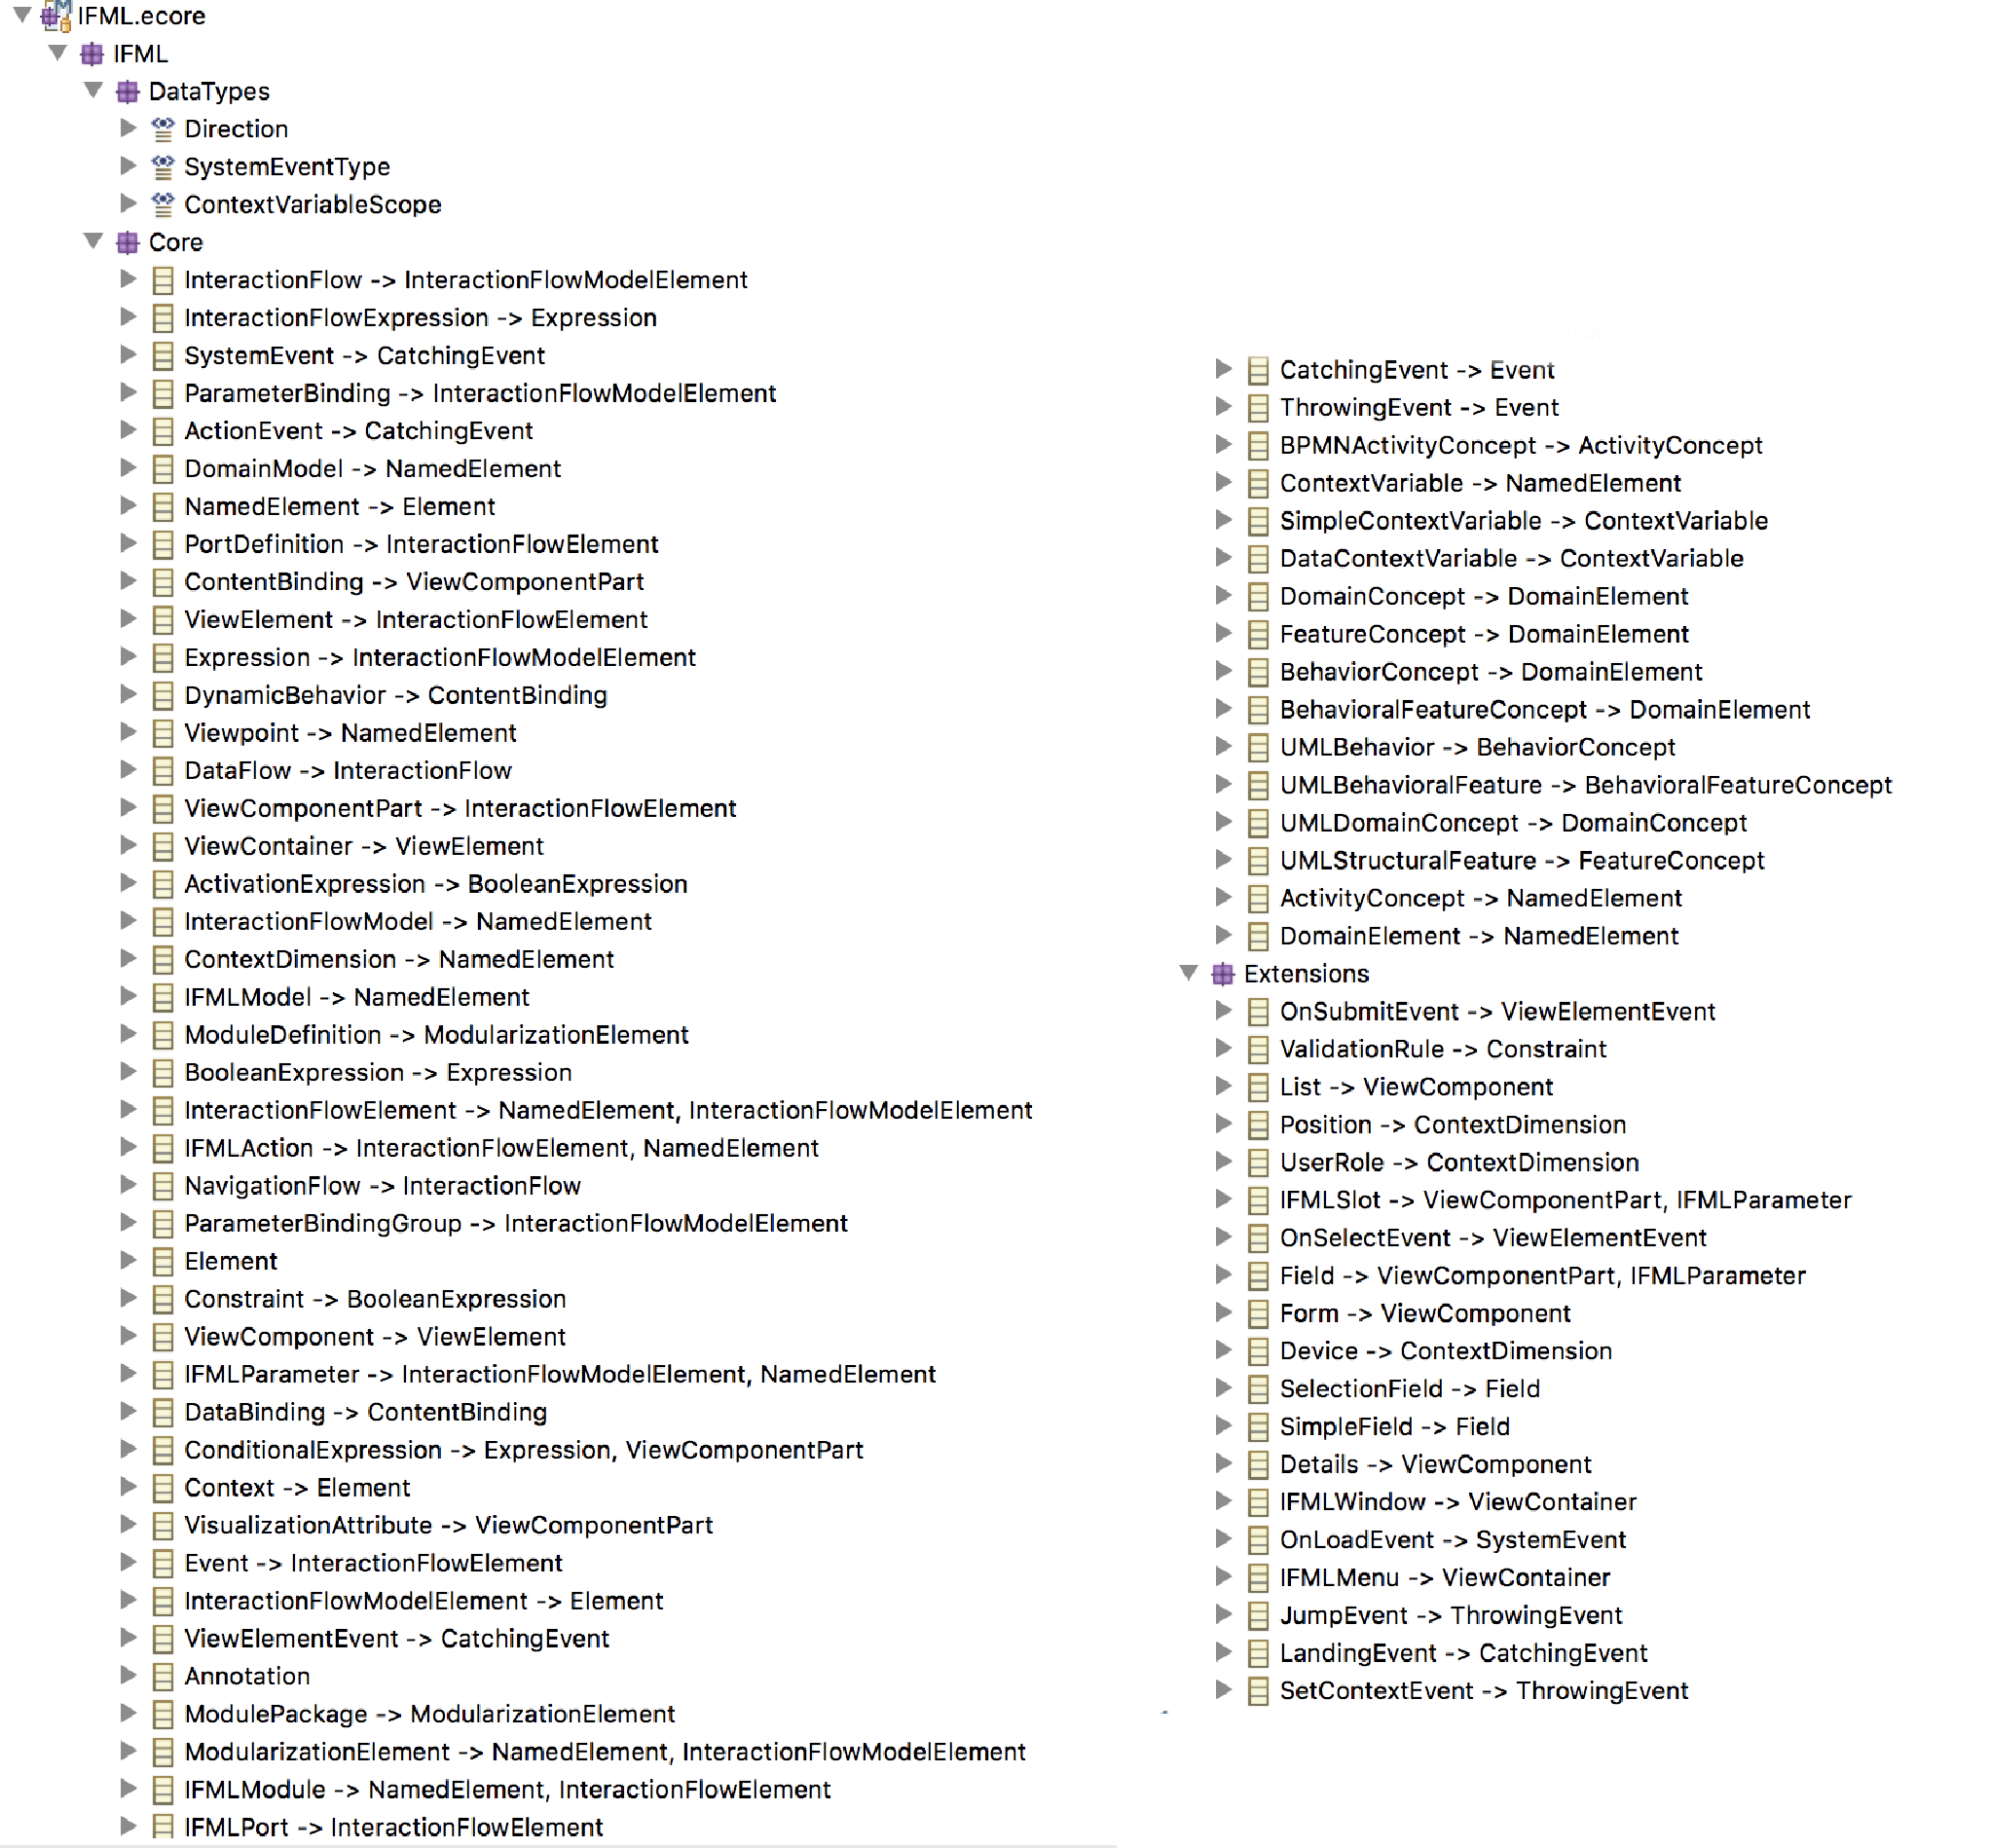
\includegraphics[width=16cm]{images/diagrams/ifml-ecore.png}
  \caption{IFML metamodel in EMF}
  \label{fig:ifml-ecore-representation}
\end{figure}
\vspace{0.5cm}

By using the primitive data types from the UML metamodel and a UML representation for the IFML Domain Model, the IFML metamodel specifies a set of UML metaclasses as the foundation for the IFML metaclasses.

\newpage
The following structure is a high-level representation of the IFML metamodel and its areas of concern:

\begin{itemize}
  \item IFML Model
  \item Interaction Flow Model
  \item Interaction Flow Elements
  \item View Elements
  \item Events
  \item Specific Events and View Components
  \item Parameters
  \item Expressions
  \item ContentBinding
\end{itemize}

Figure \ref{fig:simple-ifml-core-model} shows an excerpt of the IFML metamodel. The IFMLModel is the top-level container of all the model elements and represents an \textit{IFMLModel}. It contains an \textit{InteractionFlowModel} that is the user view of an application, a \textit{DomainModel} represented in UML, and optional ViewPoints. The concepts extending \textit{ViewContainer}, \textit{ViewComponents}, \textit{ViewComponentPart}, and \textit{ViewElementEvent} represent the visual elements of an \textit{IFMLModel}.

\vspace{0.5cm}
\begin{figure}[H]
  \centering
    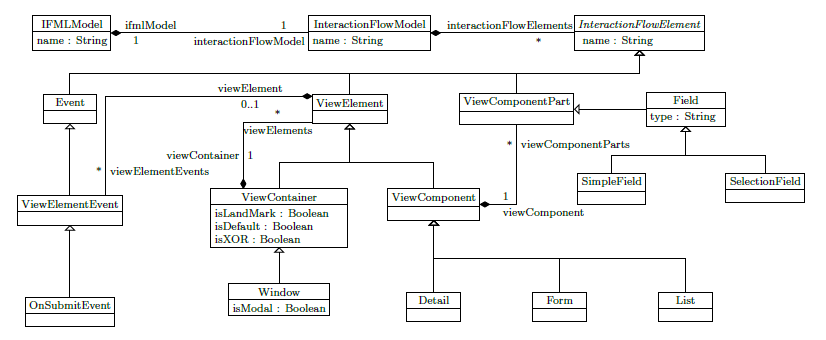
\includegraphics[width=15cm]{images/diagrams/ifml-metamodel.png}
  \caption{Class diagram of an IFML subset.}
  \label{fig:simple-ifml-core-model}
\end{figure}
\vspace{0.5cm}

\subsection{Model}

As mentioned previously, interaction flow models are described using the Interaction Flow Modelling Language and, together with the domain model and optionally viewpoints, they form the core of the \textit{IFMLModel}.

Essentially, the goal of the domain model is to offer to the interaction flow references about the available content. An example of a domain model for an e-commerce website is given in Figure~\ref{fig:domain-model-uml-ecommerce}.

\vspace{0.5cm}
\begin{figure}[H]
  \centering
    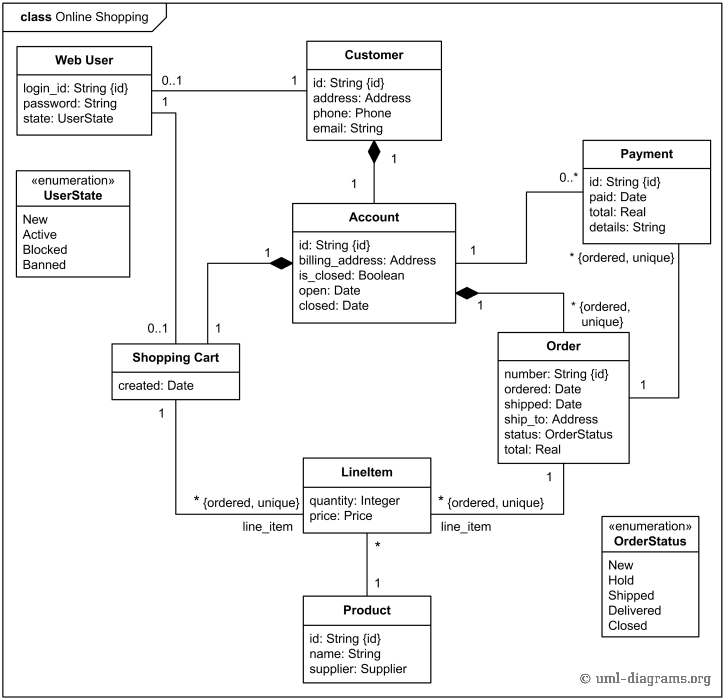
\includegraphics[width=12cm]{images/diagrams/domain-model-uml-ecommerce.png}
  \caption{Example of a Domain Model Class Diagram for an eCommerce website}
  \label{fig:domain-model-uml-ecommerce}
\end{figure}
\vspace{0.5cm}

Although some partial \textit{IFMLModel} representations for the Madison Island eCommerce platform have already been introduced in \ref{navigational-modeling-for-the-web}, in this subsection we explore the most important ones in more detail and with a broader approach that is not strictly related to the navigational modeling. Our final goal is to build an \textit{IFMLModel} which would represent the main pages and website interactions, taking advantage of the IFML metamodel described just above.

\subsubsection{Global overview}

The Madison Island Interaction Model is formed by a different combination of \textit{IFMLWindow} elements connected through \textit{IFMLAction}s reacting to distinct \textit{Events} with different \textit{ParameterBindings}. The detail of the modeling is contextual to the purpose of this work. Consequently, we have limited the inclusion of the possible interactions and elements presented on the website to the IFMLModel. In so doing, we keep the model design lightweight and reduce its complexity. Overall, the main \textit{IFMLWindow} standalone nodes have been described with more detail when compared to other shared \textit{ViewContainer} elements, such as the Header and the Footer. In Figure \ref{fig:ifml-before-global}, a visual representation of the IFMLDiagram corresponding to the main \textit{IFMLModel} for the Madison Island eCommerce platform is presented.

\vspace{0.5cm}
\begin{figure}[H]
  \centering
    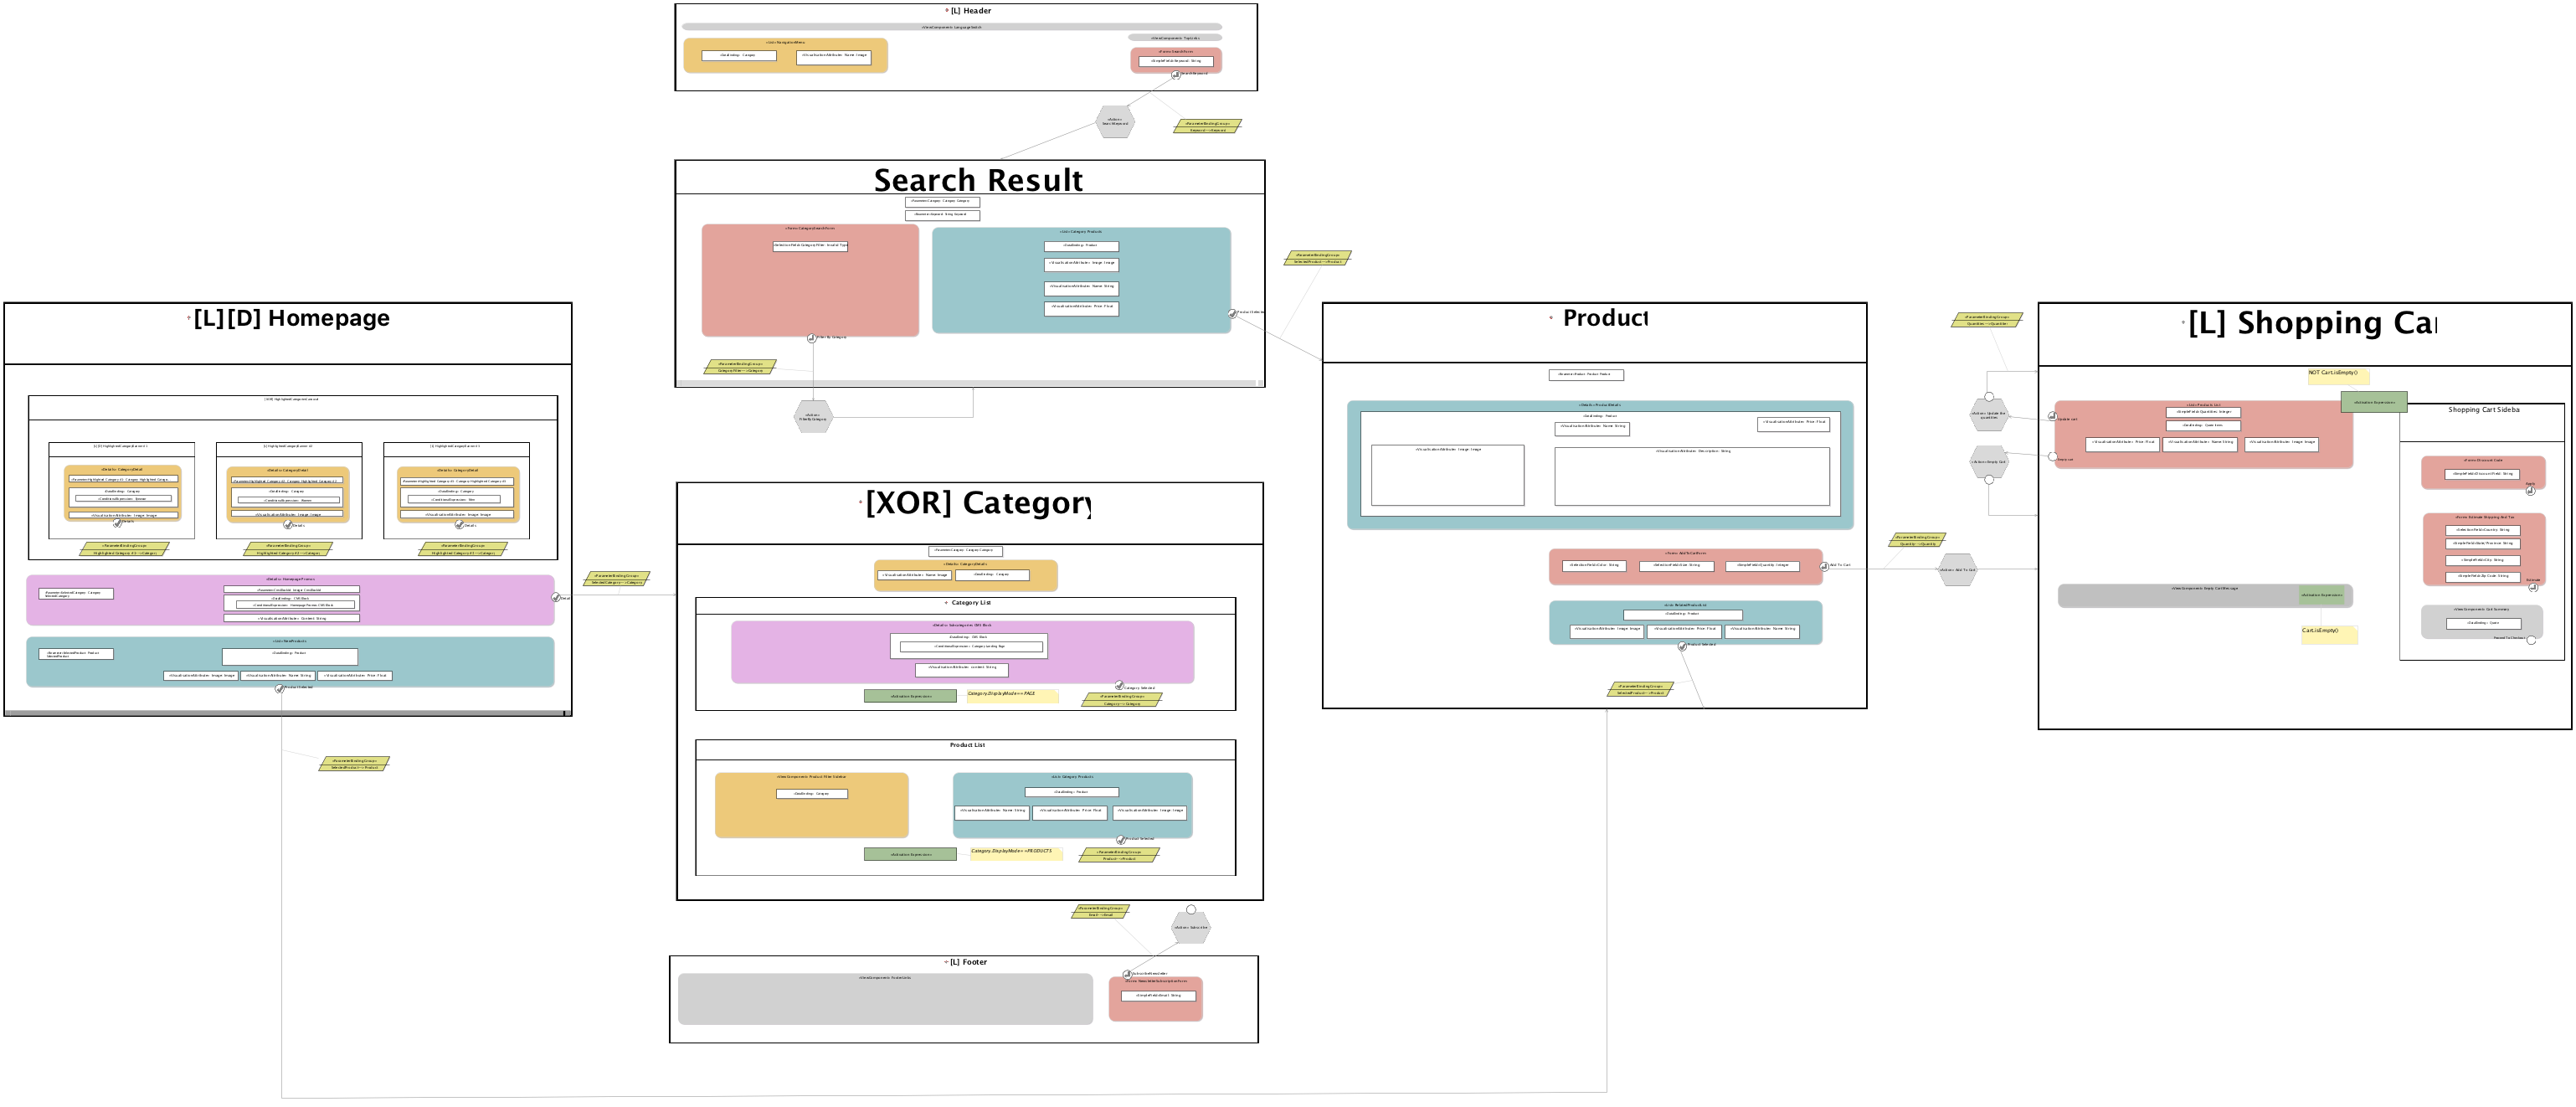
\includegraphics[height=6.5cm] {images/diagrams/before/ifml-global.png}
  \caption{Main Madison Island IFML Diagram overview}
  \label{fig:ifml-before-global}
\end{figure}
\vspace{0.5cm}
\newpage
\subsubsection{Homepage}

The Madison Island Interaction Model for the Homepage (Figure \ref{fig:desktop-before-homepage} and \ref{fig:ifml-before-homepage}) is composed by a parent \textit{IFMLWindow} element, which contains three children elements: another \textit{IFMLWindow} for the Highlighted Categories Carousel, a \textit{Detail View Component} for the Homepage promos CMS Block, and a \textit{List View Component} for the New Products sections that is bound to the Product Entity of the \textit{Domain Model} . The parent HighlightedCategoriesCarousel \textit{IFMLWindow} has the \textit{isXOR} property set to true, representing three exclusive main configurations for the initial screen within the carousel mechanism. Each \textit{Data Binding} within all these banner components is limited by a \textit{Conditional Expressions} defining the instance of the content to show.

\vspace{0.5cm}
\begin{figure}[H]
  \centering
    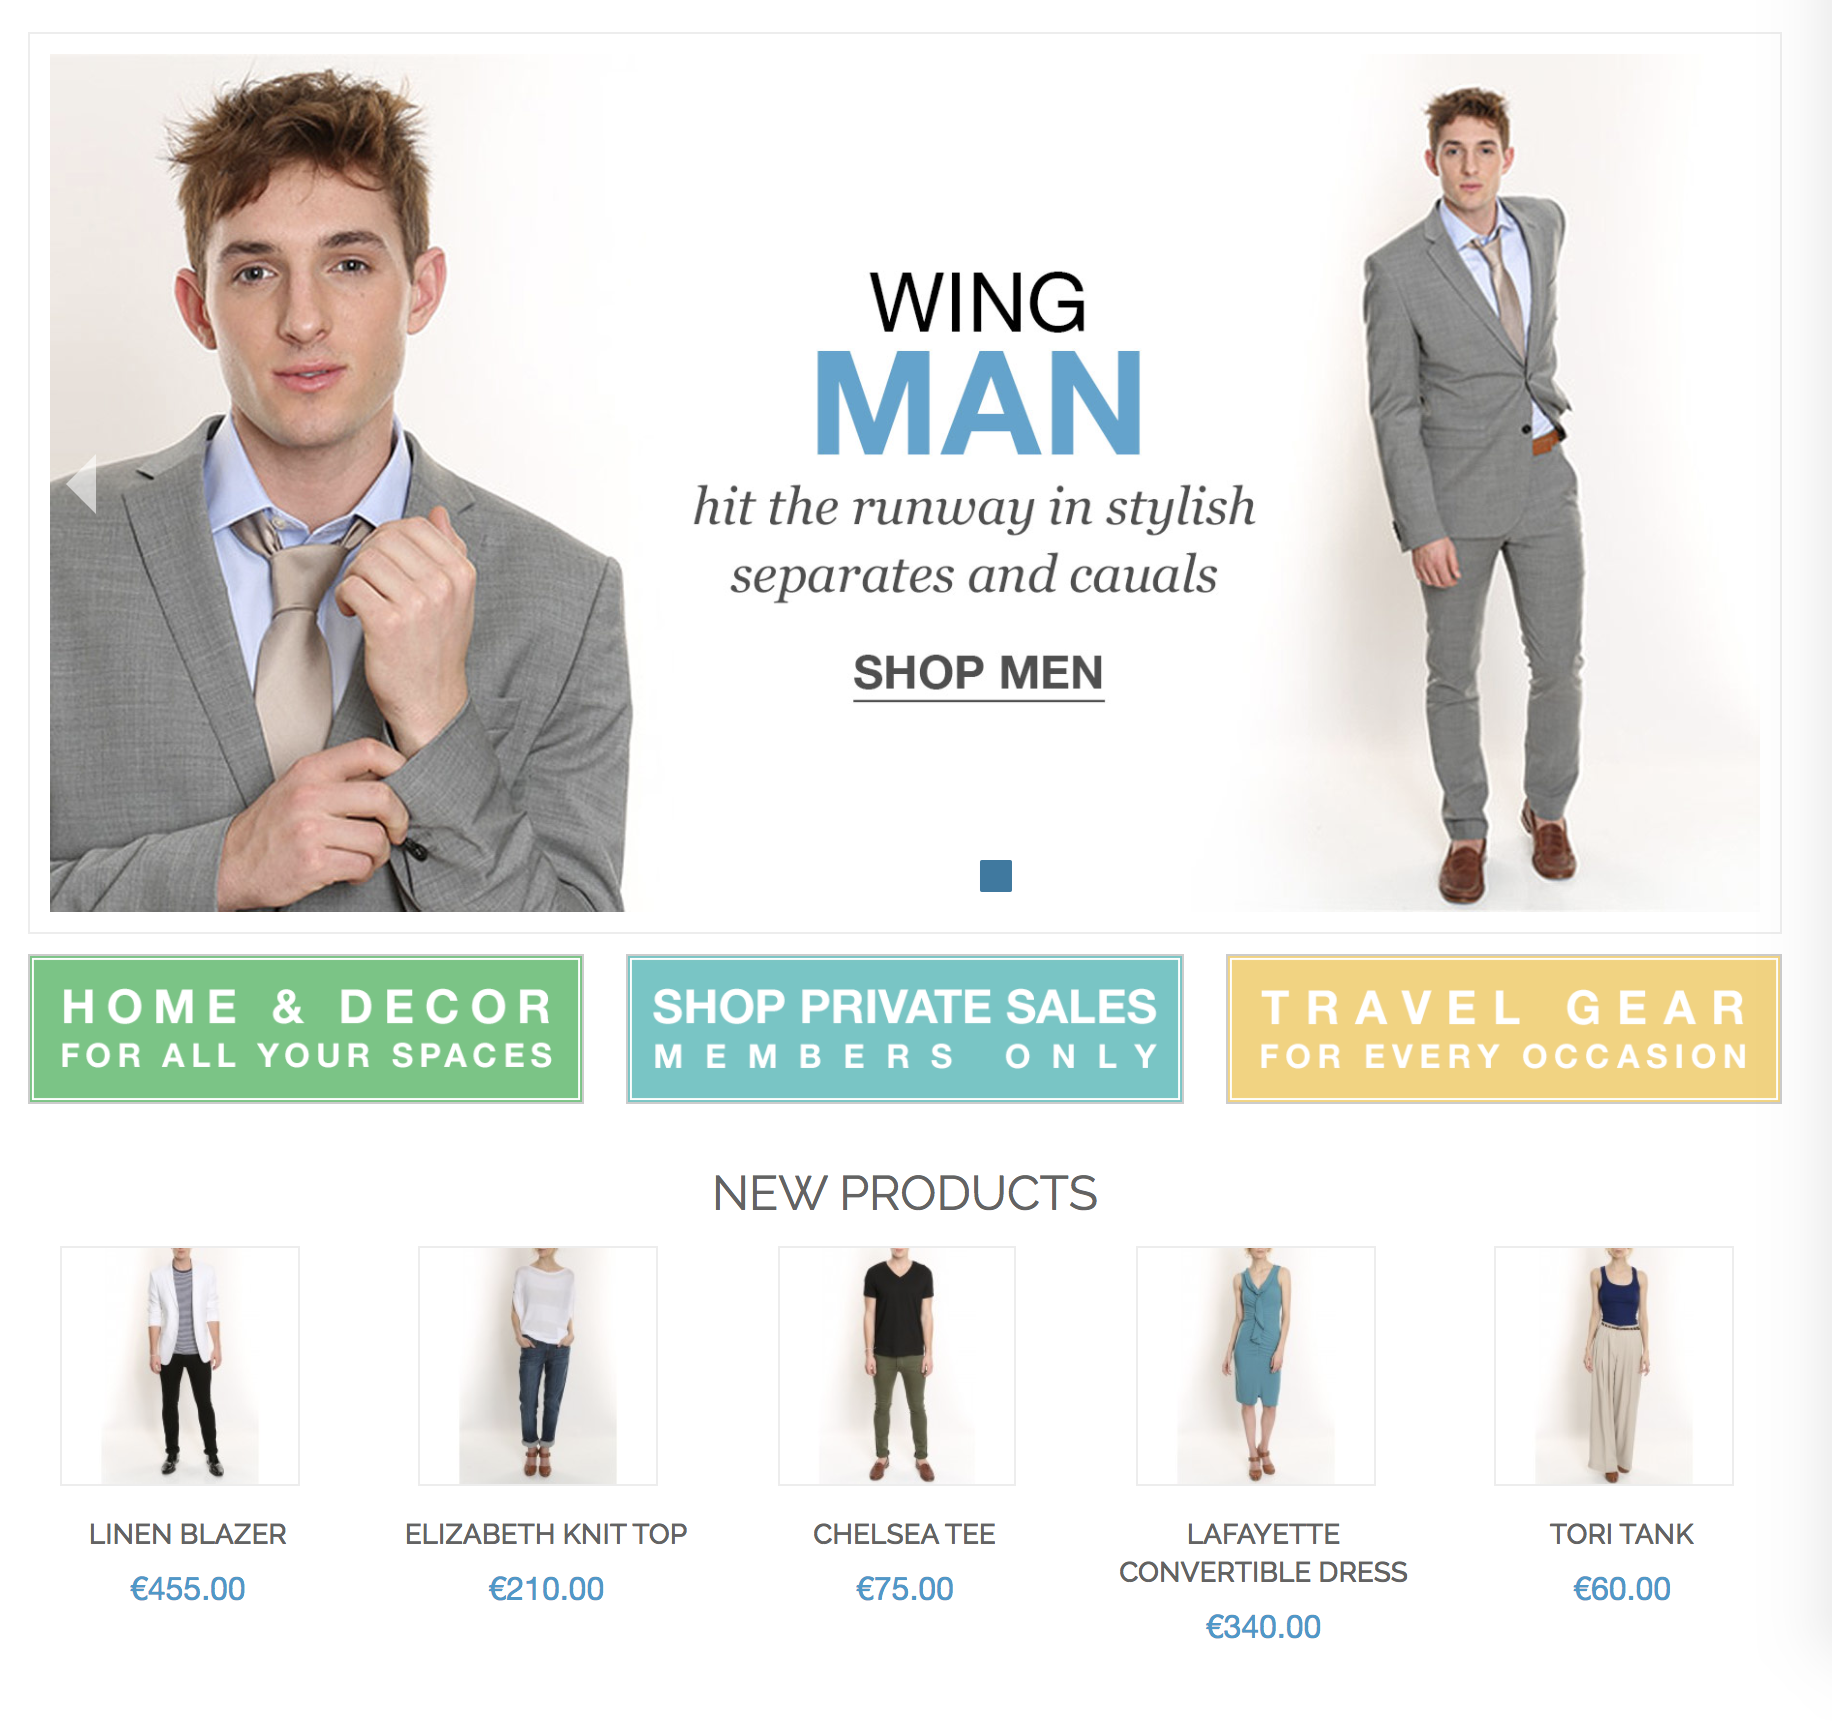
\includegraphics[width=14cm]{images/diagrams/before/desktop-homepage.png}
  \caption{Homepage Desktop Version}
  \label{fig:desktop-before-homepage}
\end{figure}
\vspace{0.5cm}

\begin{figure}[H]
  \centering
    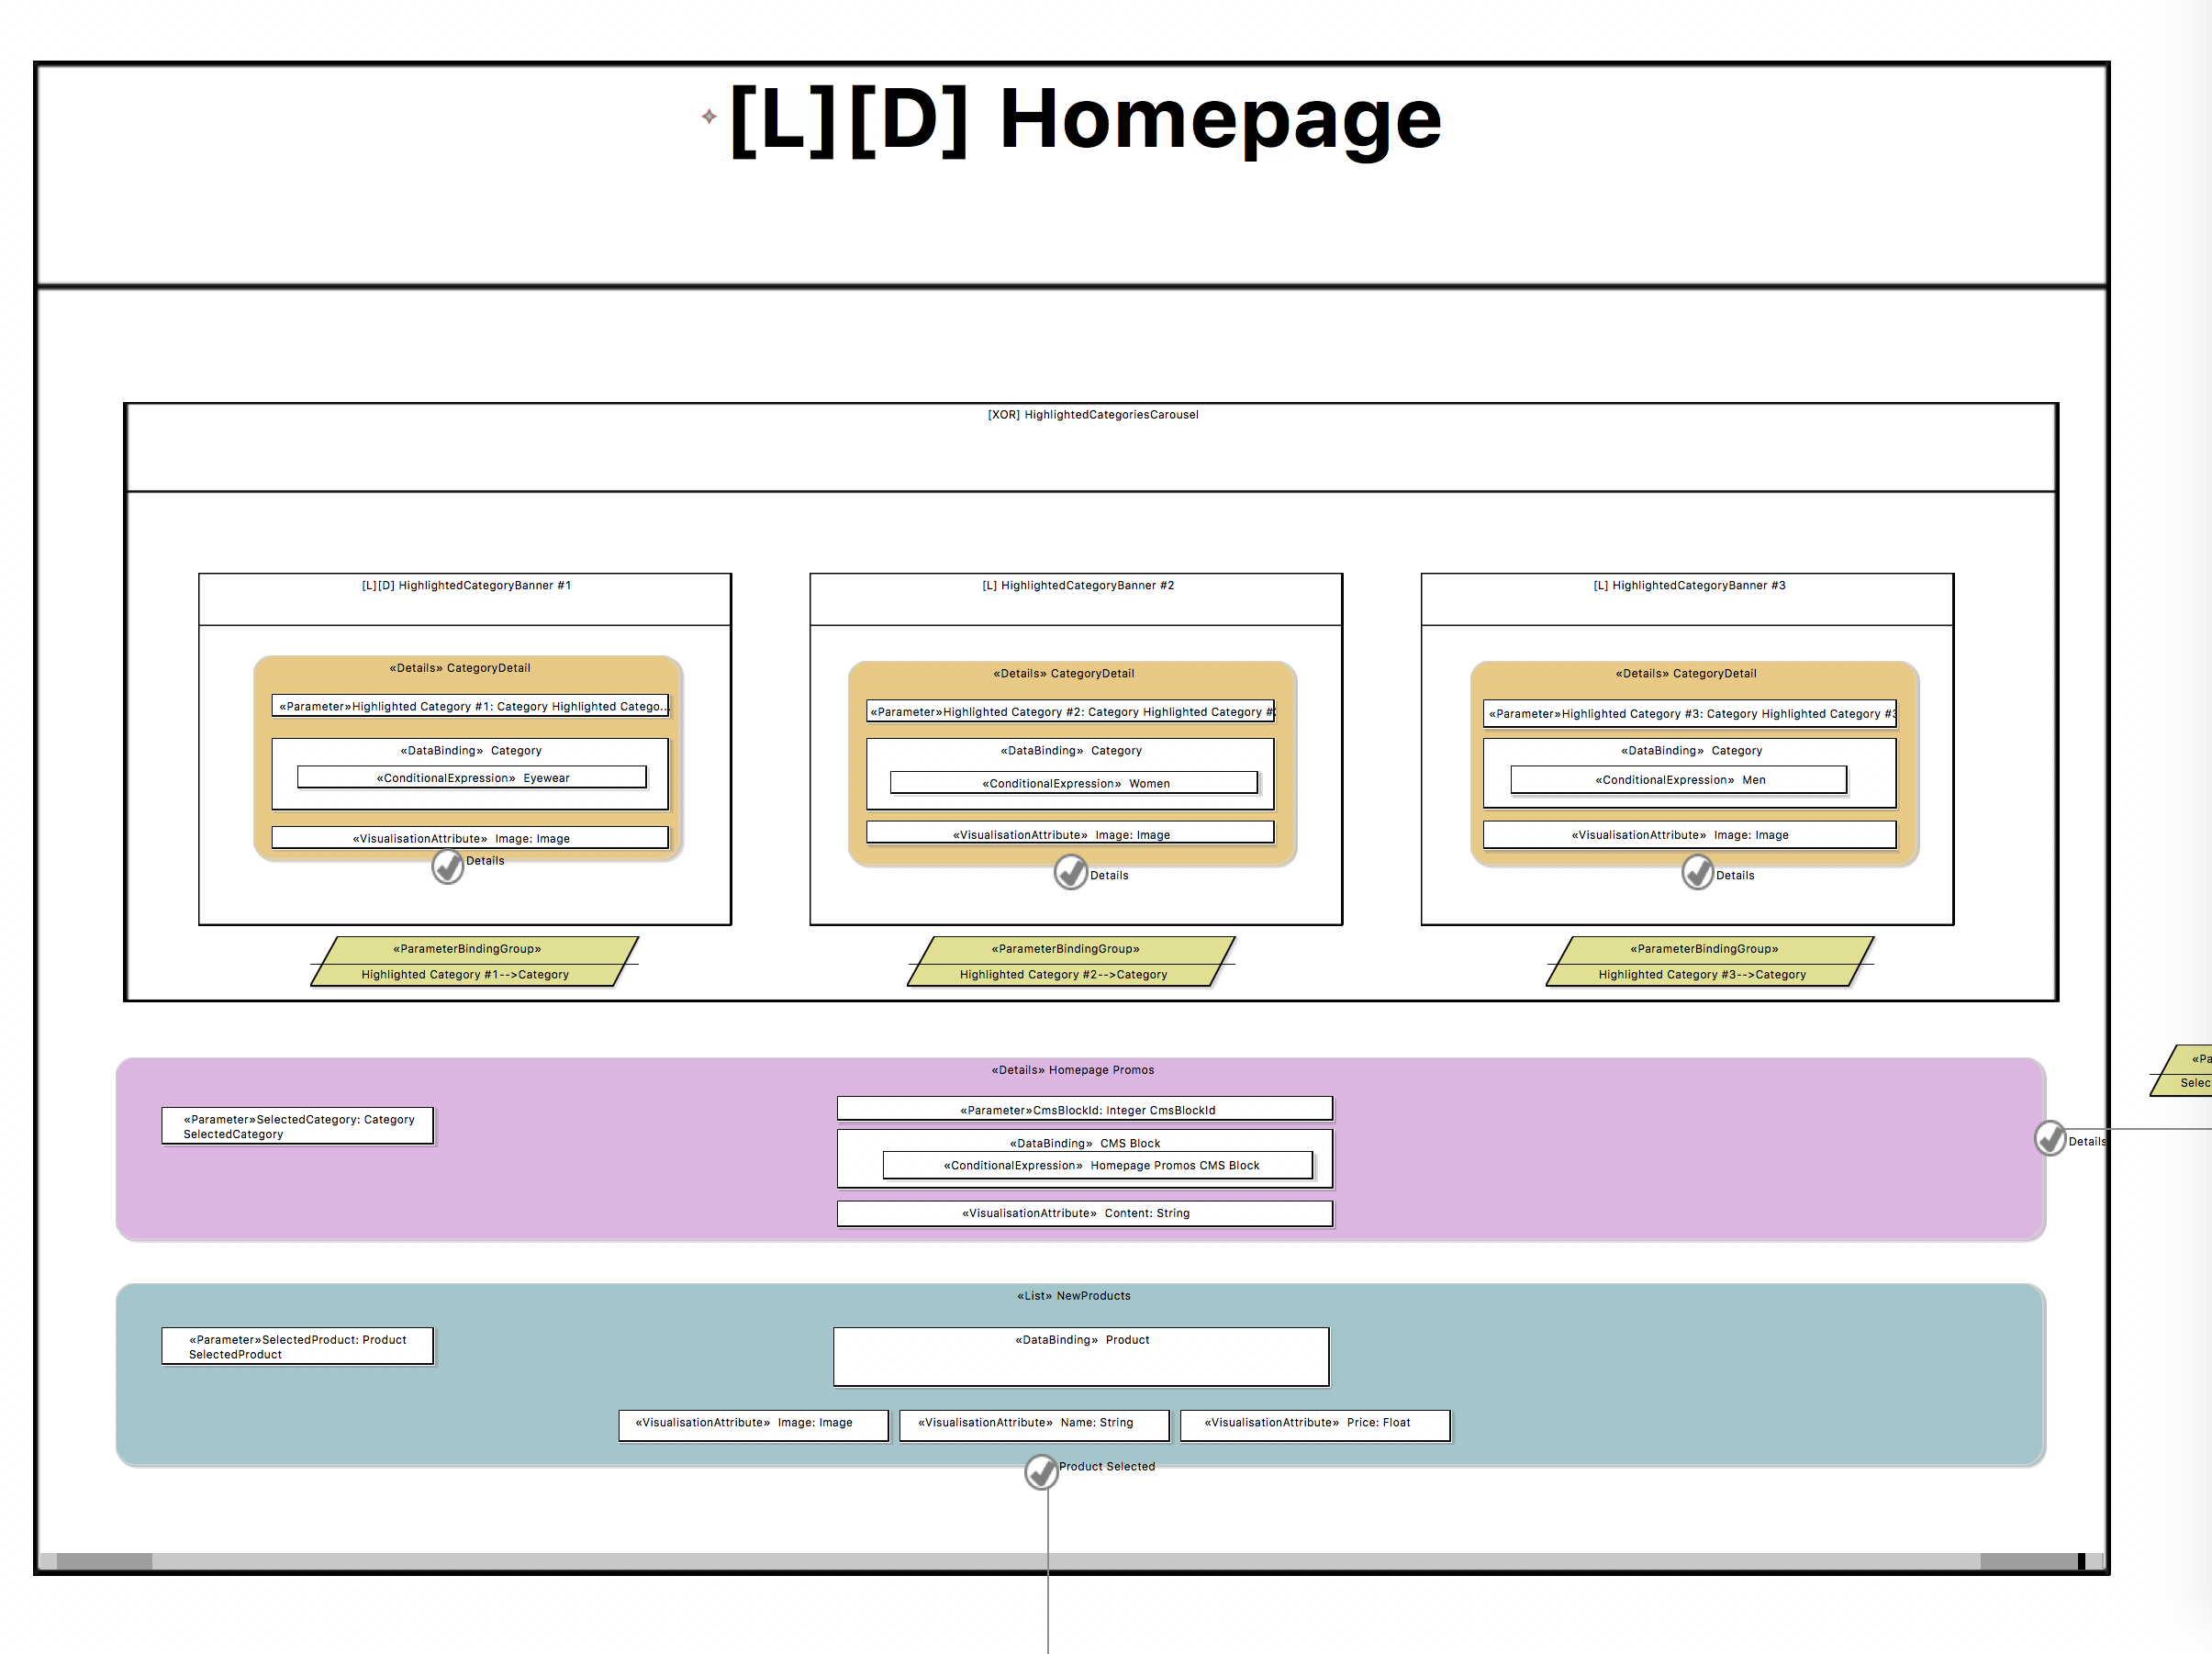
\includegraphics[width=14cm]{images/diagrams/before/ifml-homepage.png}
  \caption{Homepage IFML Diagram}
  \label{fig:ifml-before-homepage}
\end{figure}
\vspace{0.5cm}

The following snippet of code is an extract from the \textit{IFMLModel} for the first HighlighedCategoryBanner \textit{View Container} element: 
\vspace{0.5cm}
\lstset{language=XML}
\begin{lstlisting} 
      <viewElements xsi:type="ext:Details"  name="CategoryDetail">
        <parameters  name="Highlighted Category #1" direction="inout">
          <constraints  language="SQL" body="Category.ID=18"/>
        </parameters>
        <viewElementEvents xsi:type="ext:OnSelectEvent"  name="Details" viewElement="//@interactionFlowModel/@interactionFlowModelElements.0/@viewElements.0/@viewElements.0">
          <outInteractionFlows xsi:type="core:NavigationFlow"  targetInteractionFlowElement="//@interactionFlowModel/@interactionFlowModelElements.6">
            <parameterBindingGroup >
              <parameterBindings  sourceParameter="//@interactionFlowModel/@interactionFlowModelElements.0/@viewElements.0/@viewElements.0/@viewElements.0/@parameters.0" targetParameter="//@interactionFlowModel/@interactionFlowModelElements.6/@parameters.0"/>
            </parameterBindingGroup>
          </outInteractionFlows>
        </viewElementEvents>
        <viewComponentParts xsi:type="core:DataBinding"  name="Category" uniformResourceIdentifier="">
          <subViewComponentParts xsi:type="core:ConditionalExpression"  language="SQL" body="Category.ID=18" name="Eyewear"/>
        </viewComponentParts>
        <viewComponentParts xsi:type="core:VisualizationAttribute"  name="Image" featureConcept="//@domainModel/@domainElements.4"/>
      </viewElements>
    </viewElements>
\end{lstlisting}

The above snippet belongs to a more complex \textit{IFMLModel} hierarchy, as shown in \ref{fig:ifml-before-hierarchy-homepage}.

\vspace{0.5cm}
\begin{figure}[H]
  \centering
    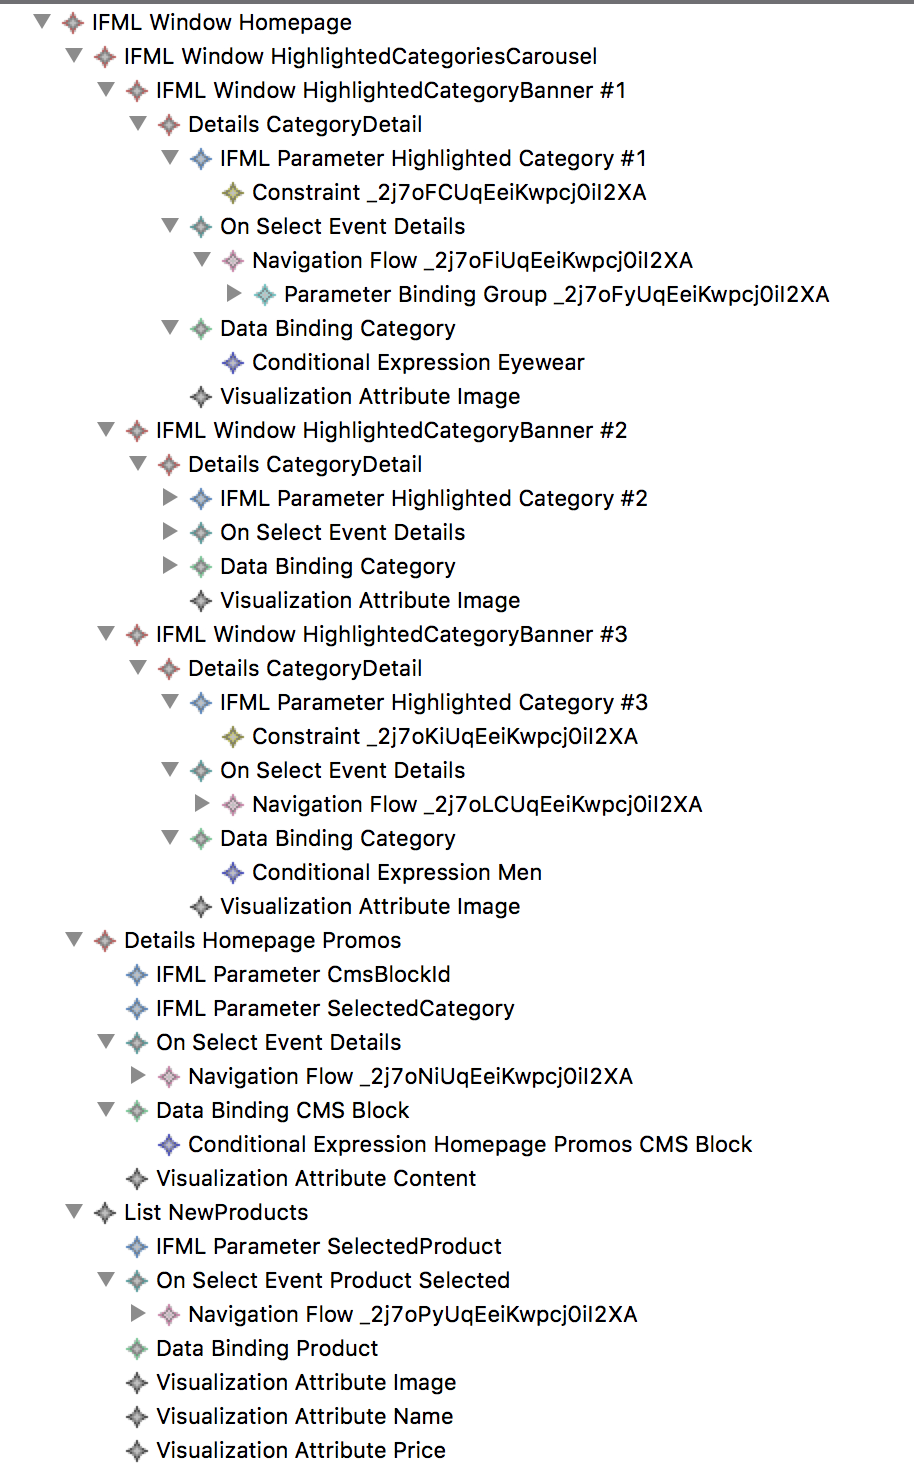
\includegraphics[width=10cm]{images/diagrams/before/ifml-hierarchy-homepage.png}
  \caption{Interaction Flow Homepage Model in EMF}
  \label{fig:ifml-before-hierarchy-homepage}
\end{figure}
\vspace{0.5cm}

\newpage
\subsubsection{Category Page}

The Madison Island Interaction Model for the Category Page (Figure \ref{fig:desktop-before-category} and \ref{fig:ifml-before-category}) is composed by a parent \textit{IFMLWindow} element with a true-ish \textit{isXOR} property, which presents information about the current category on the top of the page. Depending on the display mode property for the Category Entity, the user can be presented with two different \textit{View Containers} that are respectively activated using different \textit{Activation Expressions} based on the value of the property itself. Whilst the first scenario presents a \textit{Detail View Component} attached to a linked CMS Block, the second option shows two children view components representing both the filter sidebar and the products listing section with this last one having multiple \textit{Visualization Attribute} children nodes. These nodes indicate that the user is presented with an image used as thumbnail, a name and a price for each product belonging to the category shown.

\vspace{0.5cm}
\begin{figure}[H]
  \centering
  \subfloat[Category Page with Display Mode PAGE]{{
\includegraphics[width=8cm]{images/diagrams/before/desktop-category1.png} }}%
  \qquad
  \subfloat[Category Page with Display Mode PRODUCTS]{{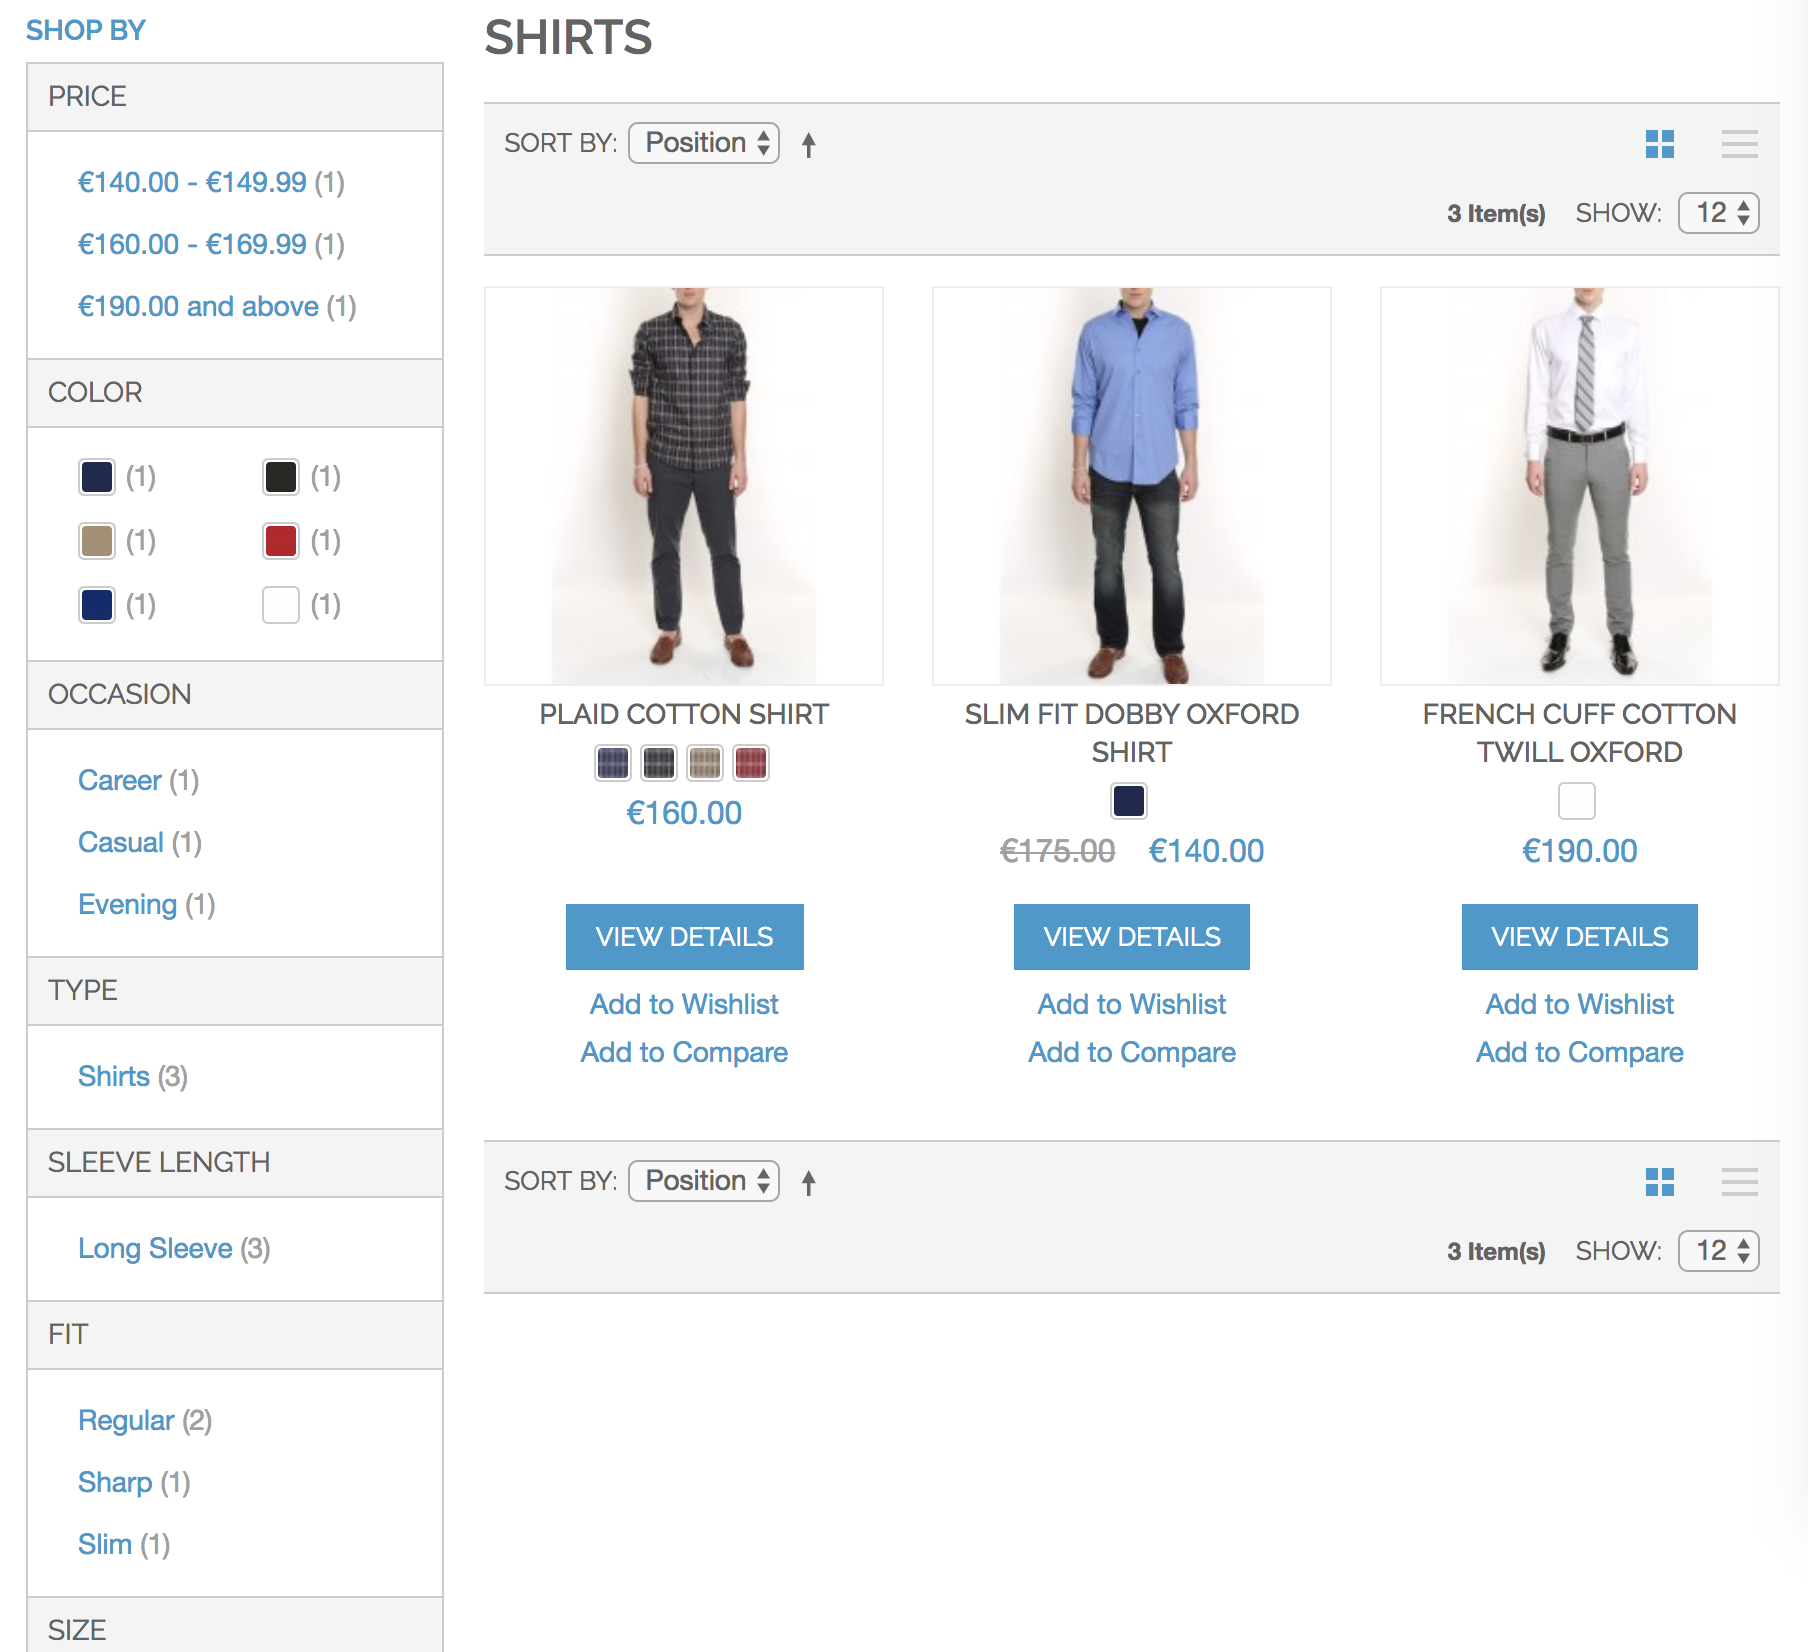
\includegraphics[width=8cm]{images/diagrams/before/desktop-category2.png} }}%
  \caption{Category Desktop Versions}%
  \label{fig:desktop-before-category}%
\end{figure}

\begin{figure}[H]
  \centering
    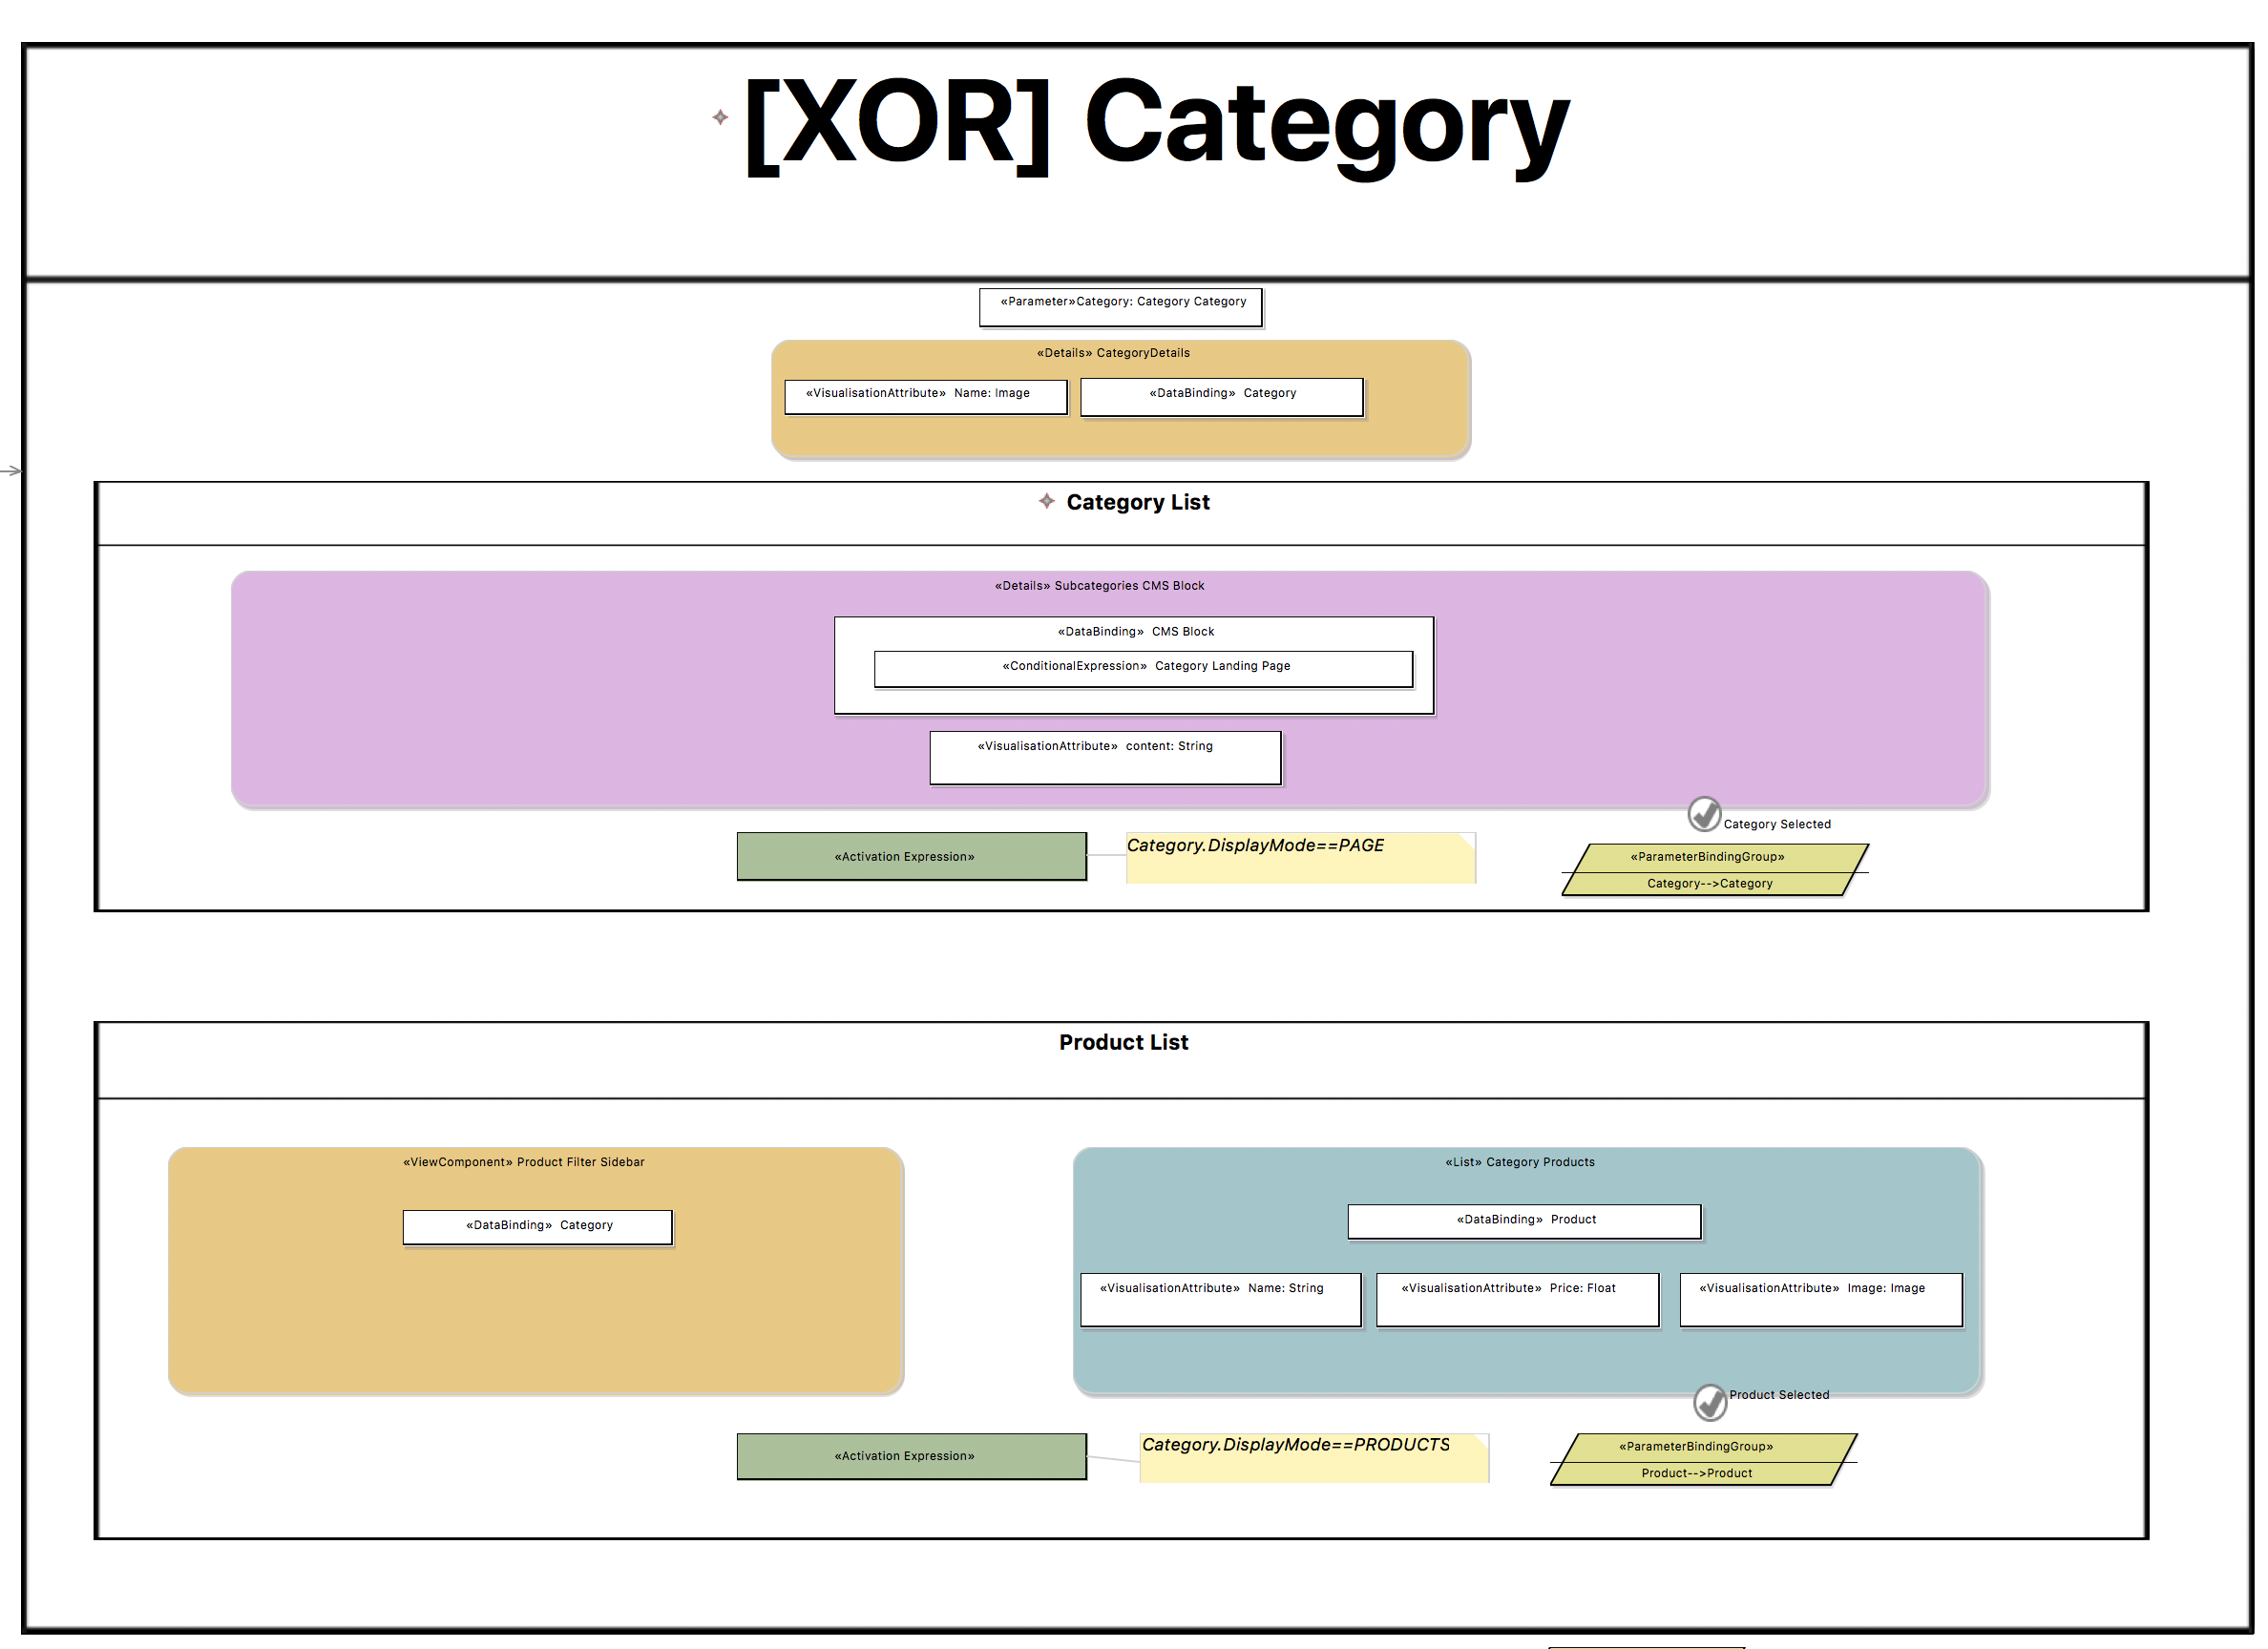
\includegraphics[width=14cm]{images/diagrams/before/ifml-category.png}
  \caption{Category IFML Diagram}
  \label{fig:ifml-before-category}
\end{figure}
\vspace{0.5cm}

The \textit{IFMLModel} code for the first Category Products List element we have just described takes this form: 
\vspace{0.5cm}
\lstset{language=XML}
\begin{lstlisting} 
    <viewElements xsi:type="ext:List"  name="Category Products">
    <viewElementEvents xsi:type="ext:OnSelectEvent"  name="Product Selected" viewElement="//@interactionFlowModel/@interactionFlowModelElements.6/@viewElements.1/@viewElements.0">
      <outInteractionFlows xsi:type="core:NavigationFlow"  targetInteractionFlowElement="//@interactionFlowModel/@interactionFlowModelElements.1">
        <parameterBindingGroup >
          <parameterBindings  sourceParameter="//@interactionFlowModel/@interactionFlowModelElements.1/@parameters.0" targetParameter="//@interactionFlowModel/@interactionFlowModelElements.1/@parameters.0"/>
        </parameterBindingGroup>
      </outInteractionFlows>
    </viewElementEvents>
    <viewComponentParts xsi:type="core:DataBinding"  name="Product" domainConcept="//@domainModel/@domainElements.3">
      <conditionalExpression  language="SQL" body="Category IN Product.Categories" name="Category Products"/>
    </viewComponentParts>
    <viewComponentParts xsi:type="core:VisualizationAttribute"  name="Image" featureConcept="//@domainModel/@domainElements.7"/>
    <viewComponentParts xsi:type="core:VisualizationAttribute"  name="Name" featureConcept="//@domainModel/@domainElements.8"/>
    <viewComponentParts xsi:type="core:VisualizationAttribute"  name="Price" featureConcept="//@domainModel/@domainElements.9"/>
  </viewElements>
  <viewElements xsi:type="core:ViewComponent"  name="Product Filter Sidebar">
    <viewComponentParts xsi:type="core:DataBinding"  name="Category"/>
  </viewElements>
</viewElements>
\end{lstlisting}

The full expanded model hierarchy for the \textit{IFMLWindow} Category element is shown in Figure \ref{fig:ifml-before-hierarchy-category}.

\vspace{0.5cm}
\begin{figure}[H]
  \centering
    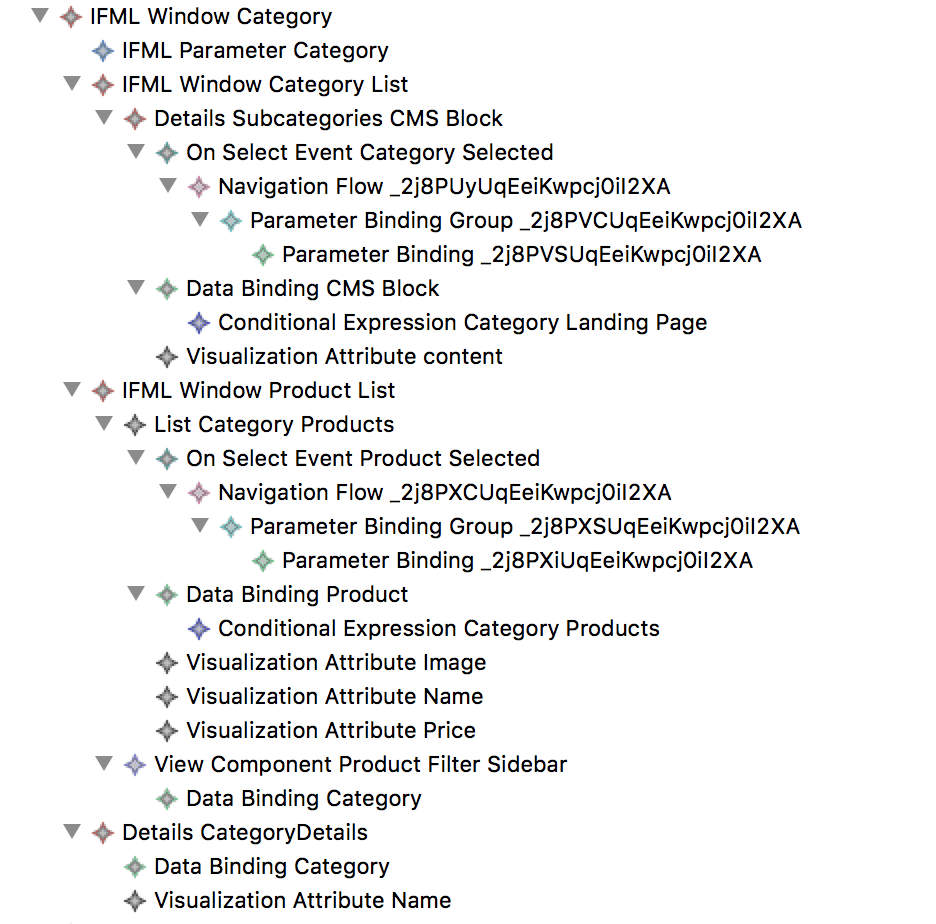
\includegraphics[width=13cm]{images/diagrams/before/ifml-hierarchy-category.png}
  \caption{Interaction Flow Category Model in EMF}
  \label{fig:ifml-before-hierarchy-category}
\end{figure}
\vspace{0.5cm}

\newpage
\subsubsection{Product Page}

The Madison Island Interaction Model for the Product page (Figure \ref{fig:desktop-before-product} and \ref{fig:ifml-before-product}) is mainly built with a single \textit{IFMLWindow} element that contains different types of \textit{View Component} nodes, the main one being a \textit{Detail View Component} instance bound to the current product data entity. The other two elements are the single \textit{Form View Component} describing the Add to Cart section and its possible interactions, and the \textit{List View Component} holding the information for the Related Product widget.

\vspace{0.5cm}
\begin{figure}[H]
  \centering
    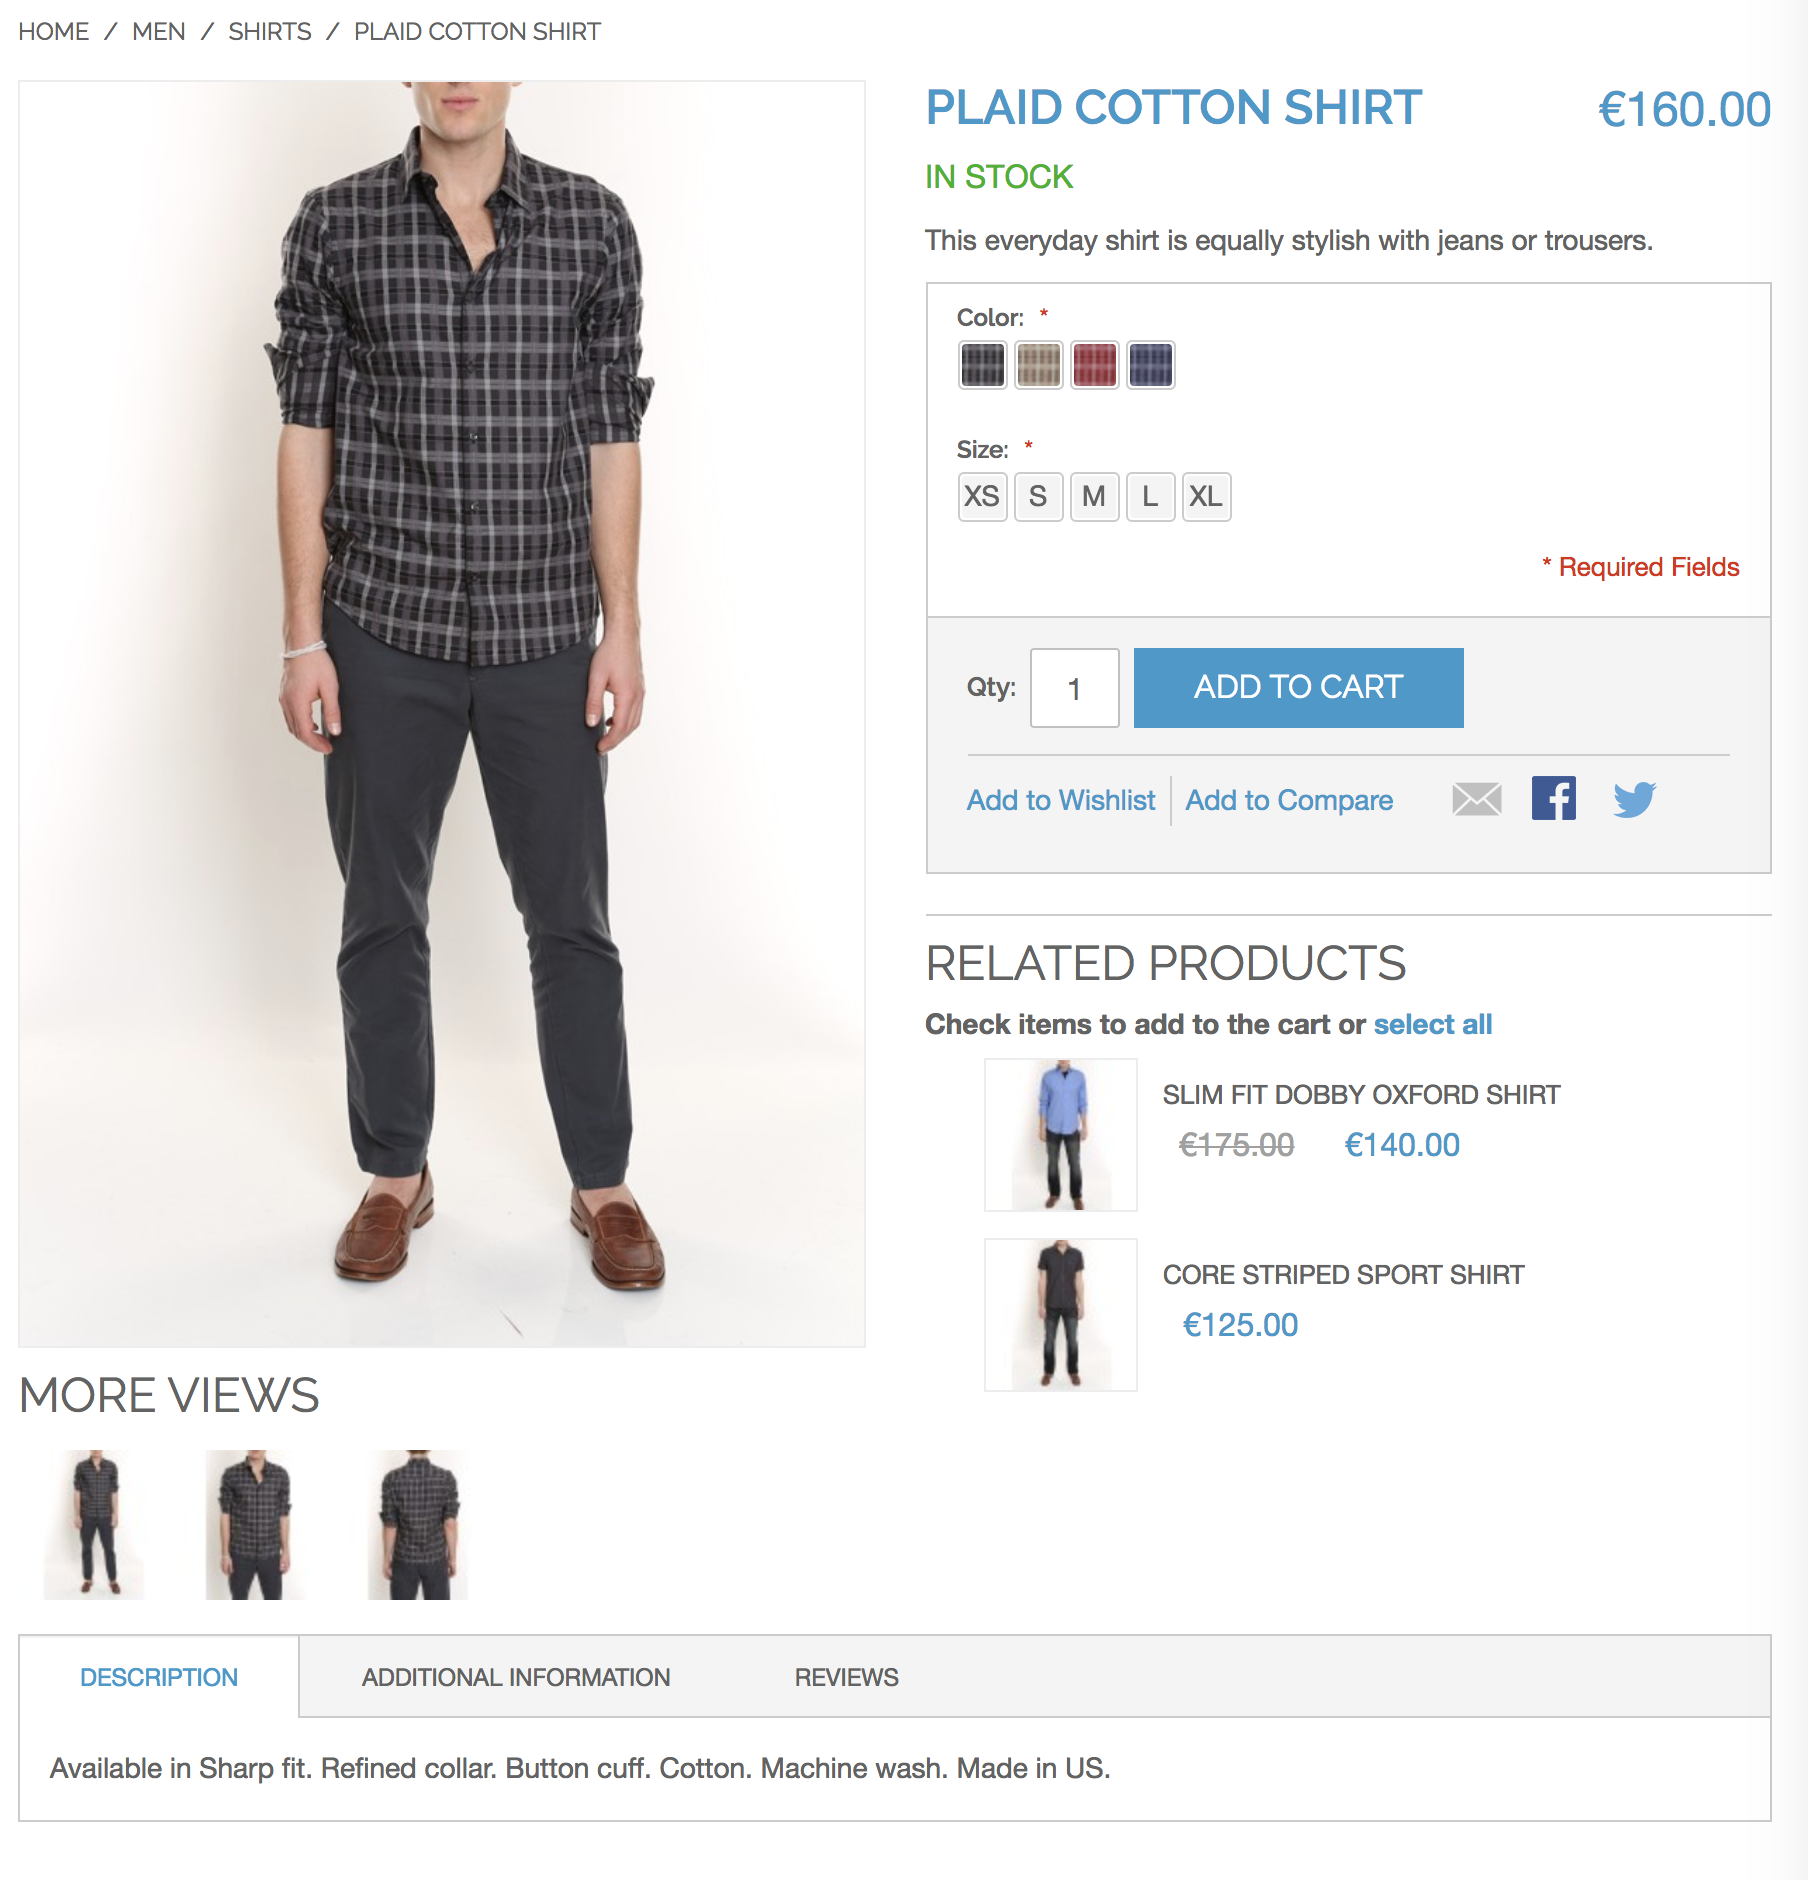
\includegraphics[width=14cm]{images/diagrams/before/desktop-product.png}
  \caption{Product Page Desktop Version}
  \label{fig:desktop-before-product}
\end{figure}

\vspace{0.5cm}
\begin{figure}[H]
  \centering
    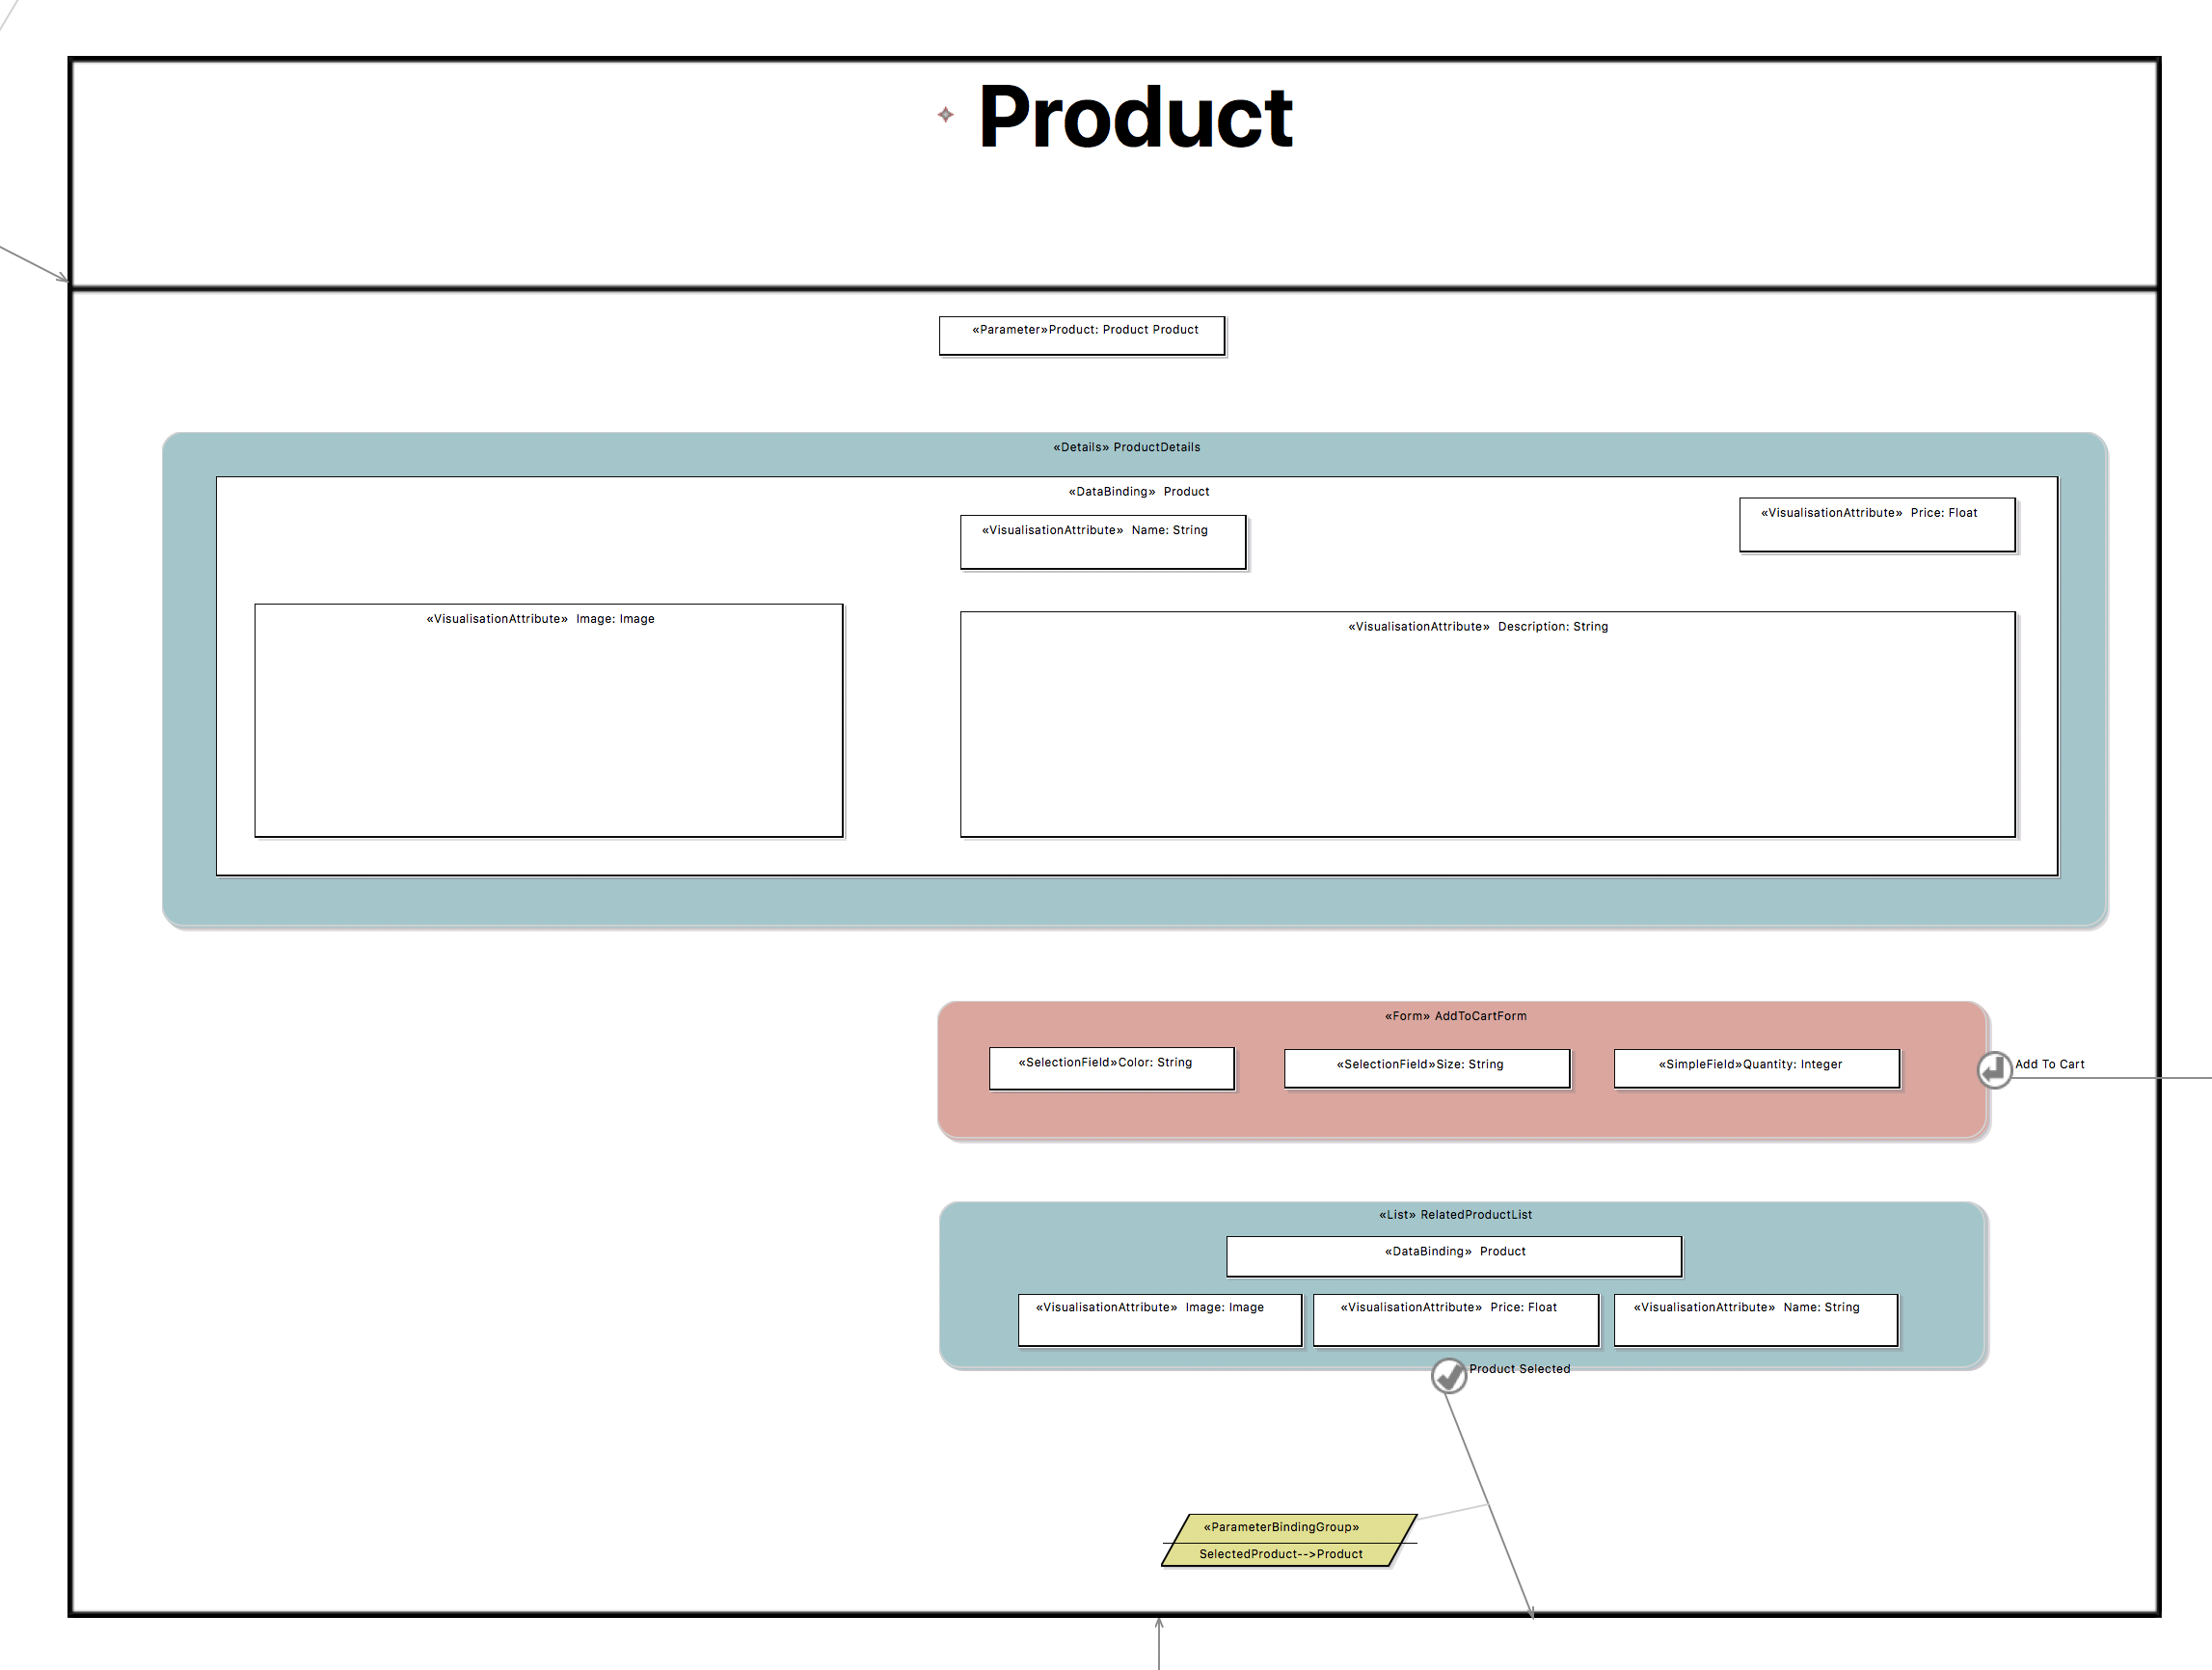
\includegraphics[width=14cm]{images/diagrams/before/ifml-product.png}
  \caption{Product Page IFML Diagram}
  \label{fig:ifml-before-product}
\end{figure}
\vspace{0.5cm}

The structure of the model just outlined produces the following \textit{IFMLModel} code:
\vspace{0.5cm}
\lstset{language=XML}
\begin{lstlisting} 
    <interactionFlowModelElements xsi:type="ext:IFMLWindow"  name="Product" inInteractionFlows="//@interactionFlowModel/@interactionFlowModelElements.1/@viewElements.2/@viewElementEvents.0/@outInteractionFlows.0 //@interactionFlowModel/@interactionFlowModelElements.0/@viewElements.2/@viewElementEvents.0/@outInteractionFlows.0 //@interactionFlowModel/@interactionFlowModelElements.10/@viewElements.0/@viewElementEvents.0/@outInteractionFlows.0 //@interactionFlowModel/@interactionFlowModelElements.6/@viewElements.1/@viewElements.0/@viewElementEvents.0/@outInteractionFlows.0">
      <parameters  name="Product" />
      <viewElements xsi:type="ext:Details"  name="ProductDetails">
        <viewComponentParts xsi:type="core:DataBinding"  name="Product" uniformResourceIdentifier="">
          <subViewComponentParts xsi:type="core:VisualizationAttribute"  name="Price" featureConcept="//@domainModel/@domainElements.9"/>
          <subViewComponentParts xsi:type="core:VisualizationAttribute"  name="Image" featureConcept="//@domainModel/@domainElements.7"/>
          <subViewComponentParts xsi:type="core:VisualizationAttribute"  name="Name" featureConcept="//@domainModel/@domainElements.8"/>
          <subViewComponentParts xsi:type="core:VisualizationAttribute"  name="Description" featureConcept="//@domainModel/@domainElements.10"/>
        </viewComponentParts>
      </viewElements>
      <viewElements xsi:type="ext:Form"  name="AddToCartForm">
        <viewElementEvents xsi:type="ext:OnSubmitEvent"  name="Add To Cart" viewElement="//@interactionFlowModel/@interactionFlowModelElements.1/@viewElements.1">
          <outInteractionFlows xsi:type="core:NavigationFlow"  targetInteractionFlowElement="//@interactionFlowModel/@interactionFlowModelElements.9">
            <parameterBindingGroup >
              <parameterBindings  sourceParameter="//@interactionFlowModel/@interactionFlowModelElements.1/@viewElements.1/@viewComponentParts.2" targetParameter="//@interactionFlowModel/@interactionFlowModelElements.1/@viewElements.1/@viewComponentParts.2"/>
            </parameterBindingGroup>
          </outInteractionFlows>
        </viewElementEvents>
        <viewComponentParts xsi:type="ext:SelectionField"  name="Color" />
        <viewComponentParts xsi:type="ext:SelectionField"  name="Size" />
        <viewComponentParts xsi:type="ext:SimpleField"  name="Quantity" />
      </viewElements>
      <viewElements xsi:type="ext:List"  name="RelatedProductList">
        <viewElementEvents xsi:type="ext:OnSelectEvent"  name="Product Selected" viewElement="//@interactionFlowModel/@interactionFlowModelElements.1/@viewElements.2">
          <outInteractionFlows xsi:type="core:NavigationFlow"  targetInteractionFlowElement="//@interactionFlowModel/@interactionFlowModelElements.1">
            <parameterBindingGroup >
              <parameterBindings  sourceParameter="//@interactionFlowModel/@interactionFlowModelElements.0/@viewElements.2/@parameters.0" targetParameter="//@interactionFlowModel/@interactionFlowModelElements.1/@parameters.0"/>
            </parameterBindingGroup>
          </outInteractionFlows>
        </viewElementEvents>
        <viewComponentParts xsi:type="core:DataBinding"  name="Product"/>
        <viewComponentParts xsi:type="core:VisualizationAttribute"  name="Image" featureConcept="//@domainModel/@domainElements.7"/>
        <viewComponentParts xsi:type="core:VisualizationAttribute"  name="Name" featureConcept="//@domainModel/@domainElements.8"/>
        <viewComponentParts xsi:type="core:VisualizationAttribute"  name="Price" featureConcept="//@domainModel/@domainElements.9"/>
      </viewElements>
    </interactionFlowModelElements>
\end{lstlisting}


The model representation of this product page structure is shown in Figure \ref{fig:ifml-before-hierarchy-product}

\vspace{0.5cm}
\begin{figure}[H]
  \centering
    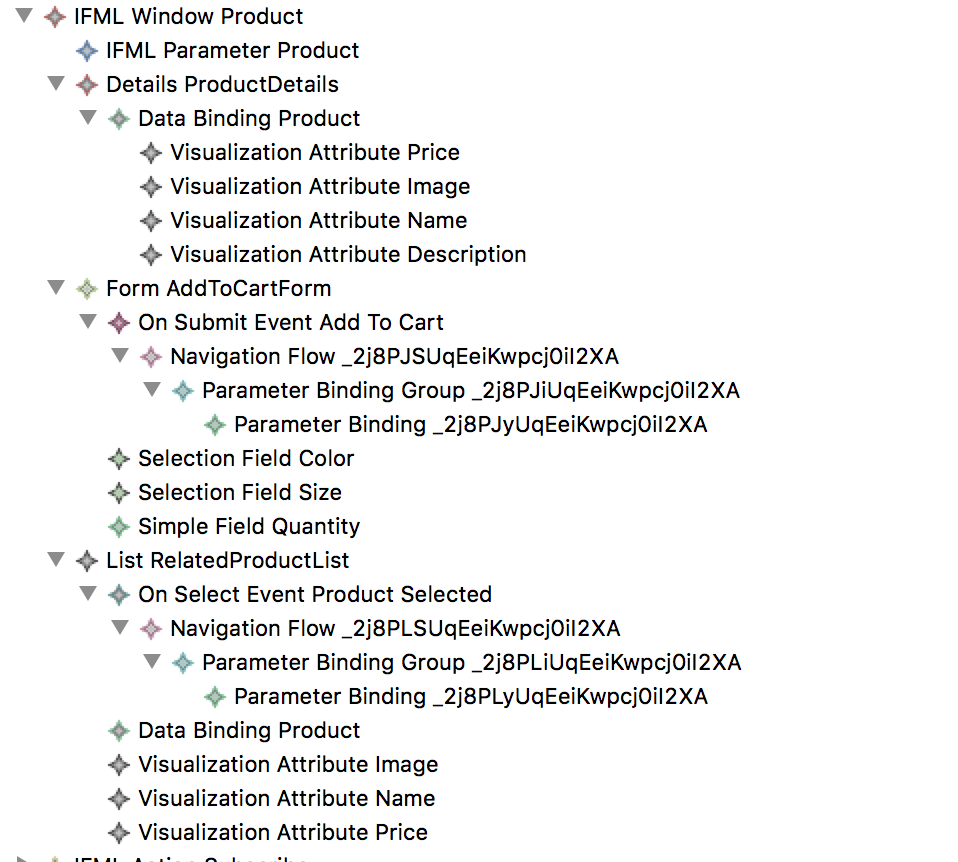
\includegraphics[width=13cm]{images/diagrams/before/ifml-hierarchy-product.png}
  \caption{Interaction Flow Product Model in EMF}
  \label{fig:ifml-before-hierarchy-product}
\end{figure}
\vspace{0.5cm}

\newpage
\subsubsection{Shopping Cart Page}
\label{shopping-cart-page-overview}
The Madison Island Interaction Model for the Shopping Cart page (Figure \ref{fig:desktop-before-shoppingcart} and \ref{fig:ifml-before-shoppingcart}) is  built with a single \textit{IFMLWindow} container with a true-ish \textit{isLandmark} property (flagging the window as accessible from everywhere) including multiple \textit{Form View Component} instances representing the sidebar interactions with the discount codes and shipping estimation widgets. Besides the sidebar, the area holding the cart status and the items in the cart information is displayed with an additional \textit{Form View Component} controlled by the \textit{Activation Condition} responsible for showing items only when the cart is not empty. The section is modelled with a \textit{Form View Component} because of the Qty \textit{SimpleInput} text fields, which allow the user to update the related item quantities or empty the whole cart at any time. Both interactions are controlled with specific \textit{IFMLAction} elements triggered on these \textit{Events}.

\vspace{0.5cm}
\begin{figure}[H]
  \centering
    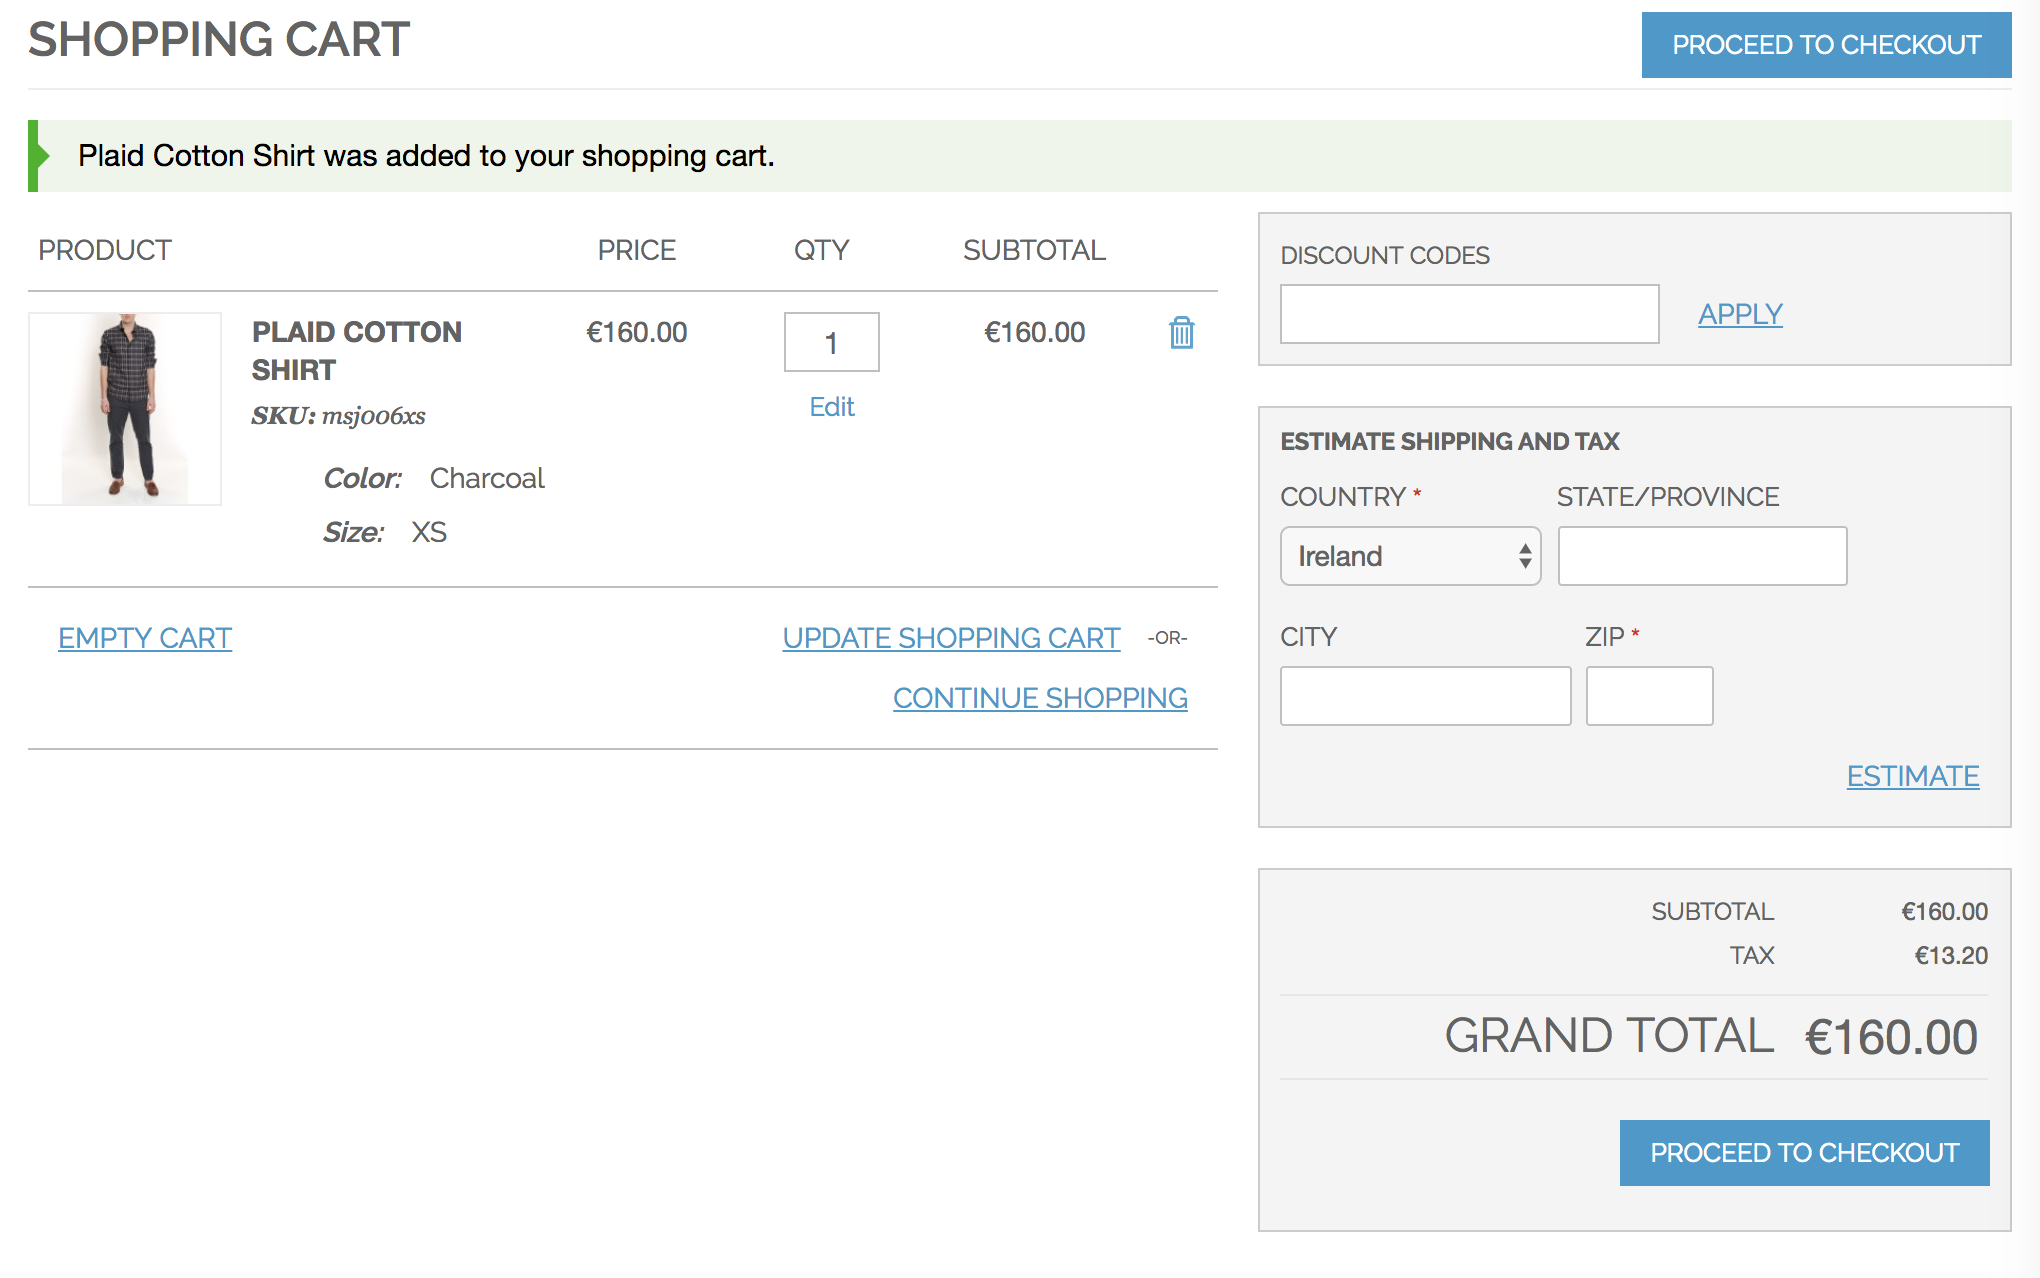
\includegraphics[width=14cm]{images/diagrams/before/desktop-shoppingcart.png}
  \caption{Shopping Cart Page Desktop Version}
  \label{fig:desktop-before-shoppingcart}
\end{figure}

\begin{figure}[H]
  \centering
    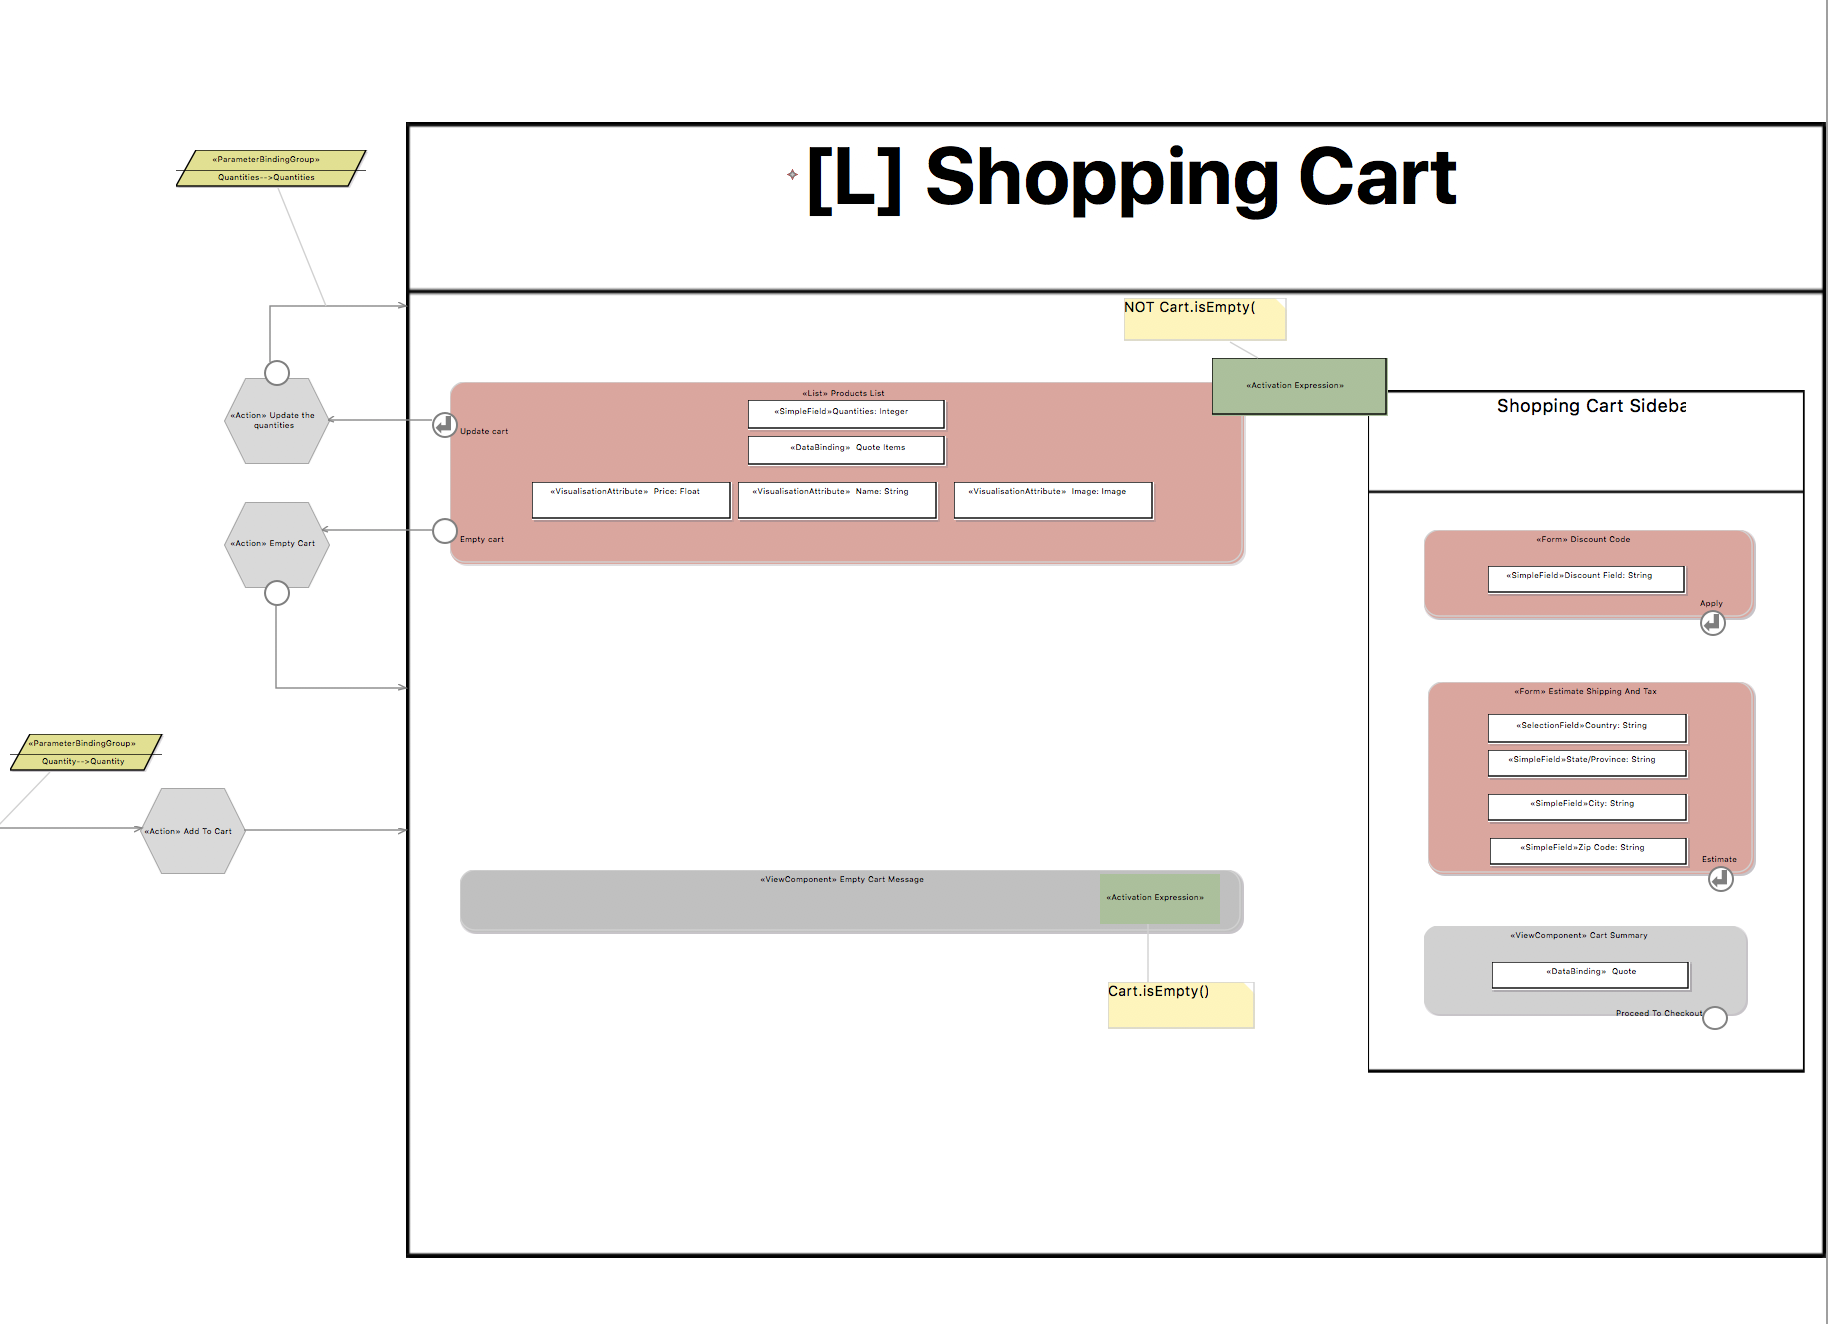
\includegraphics[width=14cm]{images/diagrams/before/ifml-shoppingcart.png}
  \caption{Shopping Cart Page IFML Diagram}
  \label{fig:ifml-before-shoppingcart}
\end{figure}

As shown in Figure \ref{fig:ifml-before-hierarchy-shoppingcart}, the Interaction Flow model representing the shopping page has the following form:
\vspace{0.5cm}
\lstset{language=XML}
\begin{lstlisting} 
    <interactionFlowModelElements xsi:type="ext:IFMLWindow"  name="Product" inInteractionFlows="//@interactionFlowModel/@interactionFlowModelElements.1/@viewElements.2/@viewElementEvents.0/@outInteractionFlows.0 //@interactionFlowModel/@interactionFlowModelElements.0/@viewElements.2/@viewElementEvents.0/@outInteractionFlows.0 //@interactionFlowModel/@interactionFlowModelElements.10/@viewElements.0/@viewElementEvents.0/@outInteractionFlows.0 //@interactionFlowModel/@interactionFlowModelElements.6/@viewElements.1/@viewElements.0/@viewElementEvents.0/@outInteractionFlows.0">
      <parameters  name="Product"/>
      <viewElements xsi:type="ext:Details"  name="ProductDetails">
        <viewComponentParts xsi:type="core:DataBinding"  name="Product" uniformResourceIdentifier="">
          <subViewComponentParts xsi:type="core:VisualizationAttribute"  name="Price" featureConcept="//@domainModel/@domainElements.9"/>
          <subViewComponentParts xsi:type="core:VisualizationAttribute"  name="Image" featureConcept="//@domainModel/@domainElements.7"/>
          <subViewComponentParts xsi:type="core:VisualizationAttribute"  name="Name" featureConcept="//@domainModel/@domainElements.8"/>
          <subViewComponentParts xsi:type="core:VisualizationAttribute"  name="Description" featureConcept="//@domainModel/@domainElements.10"/>
        </viewComponentParts>
      </viewElements>
      <viewElements xsi:type="ext:Form"  name="AddToCartForm">
        <viewElementEvents xsi:type="ext:OnSubmitEvent"  name="Add To Cart" viewElement="//@interactionFlowModel/@interactionFlowModelElements.1/@viewElements.1">
          <outInteractionFlows xsi:type="core:NavigationFlow"  targetInteractionFlowElement="//@interactionFlowModel/@interactionFlowModelElements.9">
            <parameterBindingGroup >
              <parameterBindings  sourceParameter="//@interactionFlowModel/@interactionFlowModelElements.1/@viewElements.1/@viewComponentParts.2" targetParameter="//@interactionFlowModel/@interactionFlowModelElements.1/@viewElements.1/@viewComponentParts.2"/>
            </parameterBindingGroup>
          </outInteractionFlows>
        </viewElementEvents>
        <viewComponentParts xsi:type="ext:SelectionField"  name="Color" />
        <viewComponentParts xsi:type="ext:SelectionField"  name="Size" />
        <viewComponentParts xsi:type="ext:SimpleField"  name="Quantity" />
      </viewElements>
      <viewElements xsi:type="ext:List"  name="RelatedProductList">
        <viewElementEvents xsi:type="ext:OnSelectEvent"  name="Product Selected" viewElement="//@interactionFlowModel/@interactionFlowModelElements.1/@viewElements.2">
          <outInteractionFlows xsi:type="core:NavigationFlow"  targetInteractionFlowElement="//@interactionFlowModel/@interactionFlowModelElements.1">
            <parameterBindingGroup >
              <parameterBindings  sourceParameter="//@interactionFlowModel/@interactionFlowModelElements.0/@viewElements.2/@parameters.0" targetParameter="//@interactionFlowModel/@interactionFlowModelElements.1/@parameters.0"/>
            </parameterBindingGroup>
          </outInteractionFlows>
        </viewElementEvents>
        <viewComponentParts xsi:type="core:DataBinding"  name="Product"/>
        <viewComponentParts xsi:type="core:VisualizationAttribute"  name="Image" featureConcept="//@domainModel/@domainElements.7"/>
        <viewComponentParts xsi:type="core:VisualizationAttribute"  name="Name" featureConcept="//@domainModel/@domainElements.8"/>
        <viewComponentParts xsi:type="core:VisualizationAttribute"  name="Price" featureConcept="//@domainModel/@domainElements.9"/>
      </viewElements>
    </interactionFlowModelElements>
\end{lstlisting}

The \textit{IFMLModel} representation of the Shopping Cart page structure is presented in Figure \ref{fig:ifml-before-hierarchy-shoppingcart}

\vspace{0.5cm}
\begin{figure}[H]
  \centering
    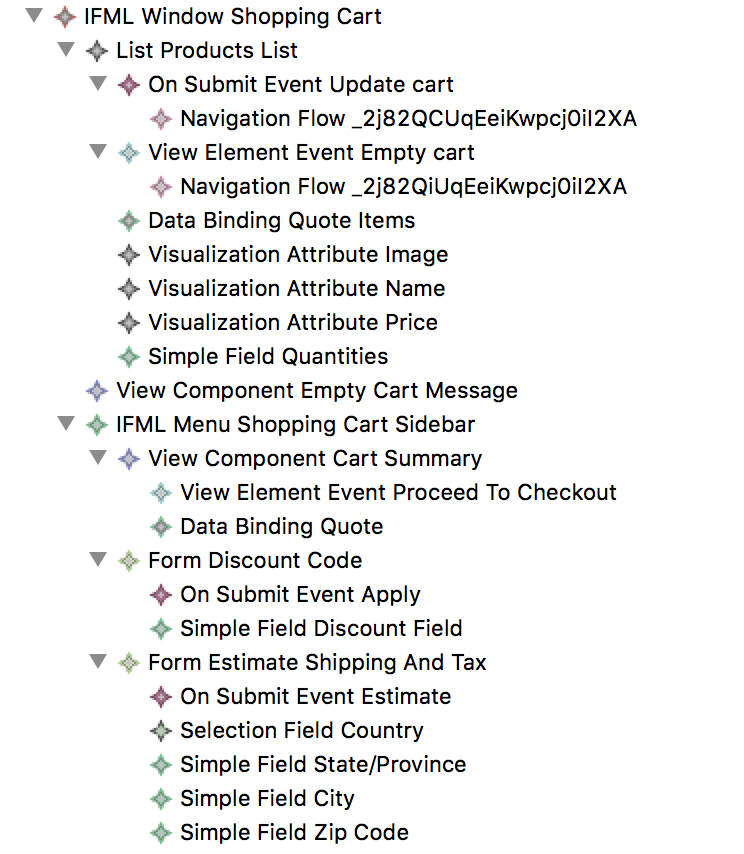
\includegraphics[width=12cm]{images/diagrams/before/ifml-hierarchy-shoppingcart.png}
  \caption{Interaction Flow Shopping Cart Model in EMF}
  \label{fig:ifml-before-hierarchy-shoppingcart}
\end{figure}
\vspace{0.5cm}

\subsubsection{Shared Elements and Interactions}

As mentioned previously, shared sections of the platform such as the Header and the Footer have been modelled as \textit{IFMLWindow} nodes reachable from any other area of the website, thus their \textit{isLandmark} attribute set to true. In more detail, the Header section contains a Navigation Menu in the form of a \textit{List View Component} with a children \textit{DataBinding} component correlated to the Category \textit{Domain Model} and a simple \textit{Form View Component} for the search mechanism. When the user performs a search submitting a keyword, the \textit{SearchKeyword} is triggered and the Search Keyword \textit{IFMLAction} is executed based on the parameters held in the associated \textit{ParameterBinding} element.  The resulting Search Results page, which presents a sidebar for filtering and a list of items matching the search, is another \textit{IFMLWindow}, whose structure resembles the "Product List Mode" for a Category Page described earlier (Figure \ref{fig:ifml-before-header-search}).

\vspace{0.5cm}
\begin{figure}[H]
  \centering
    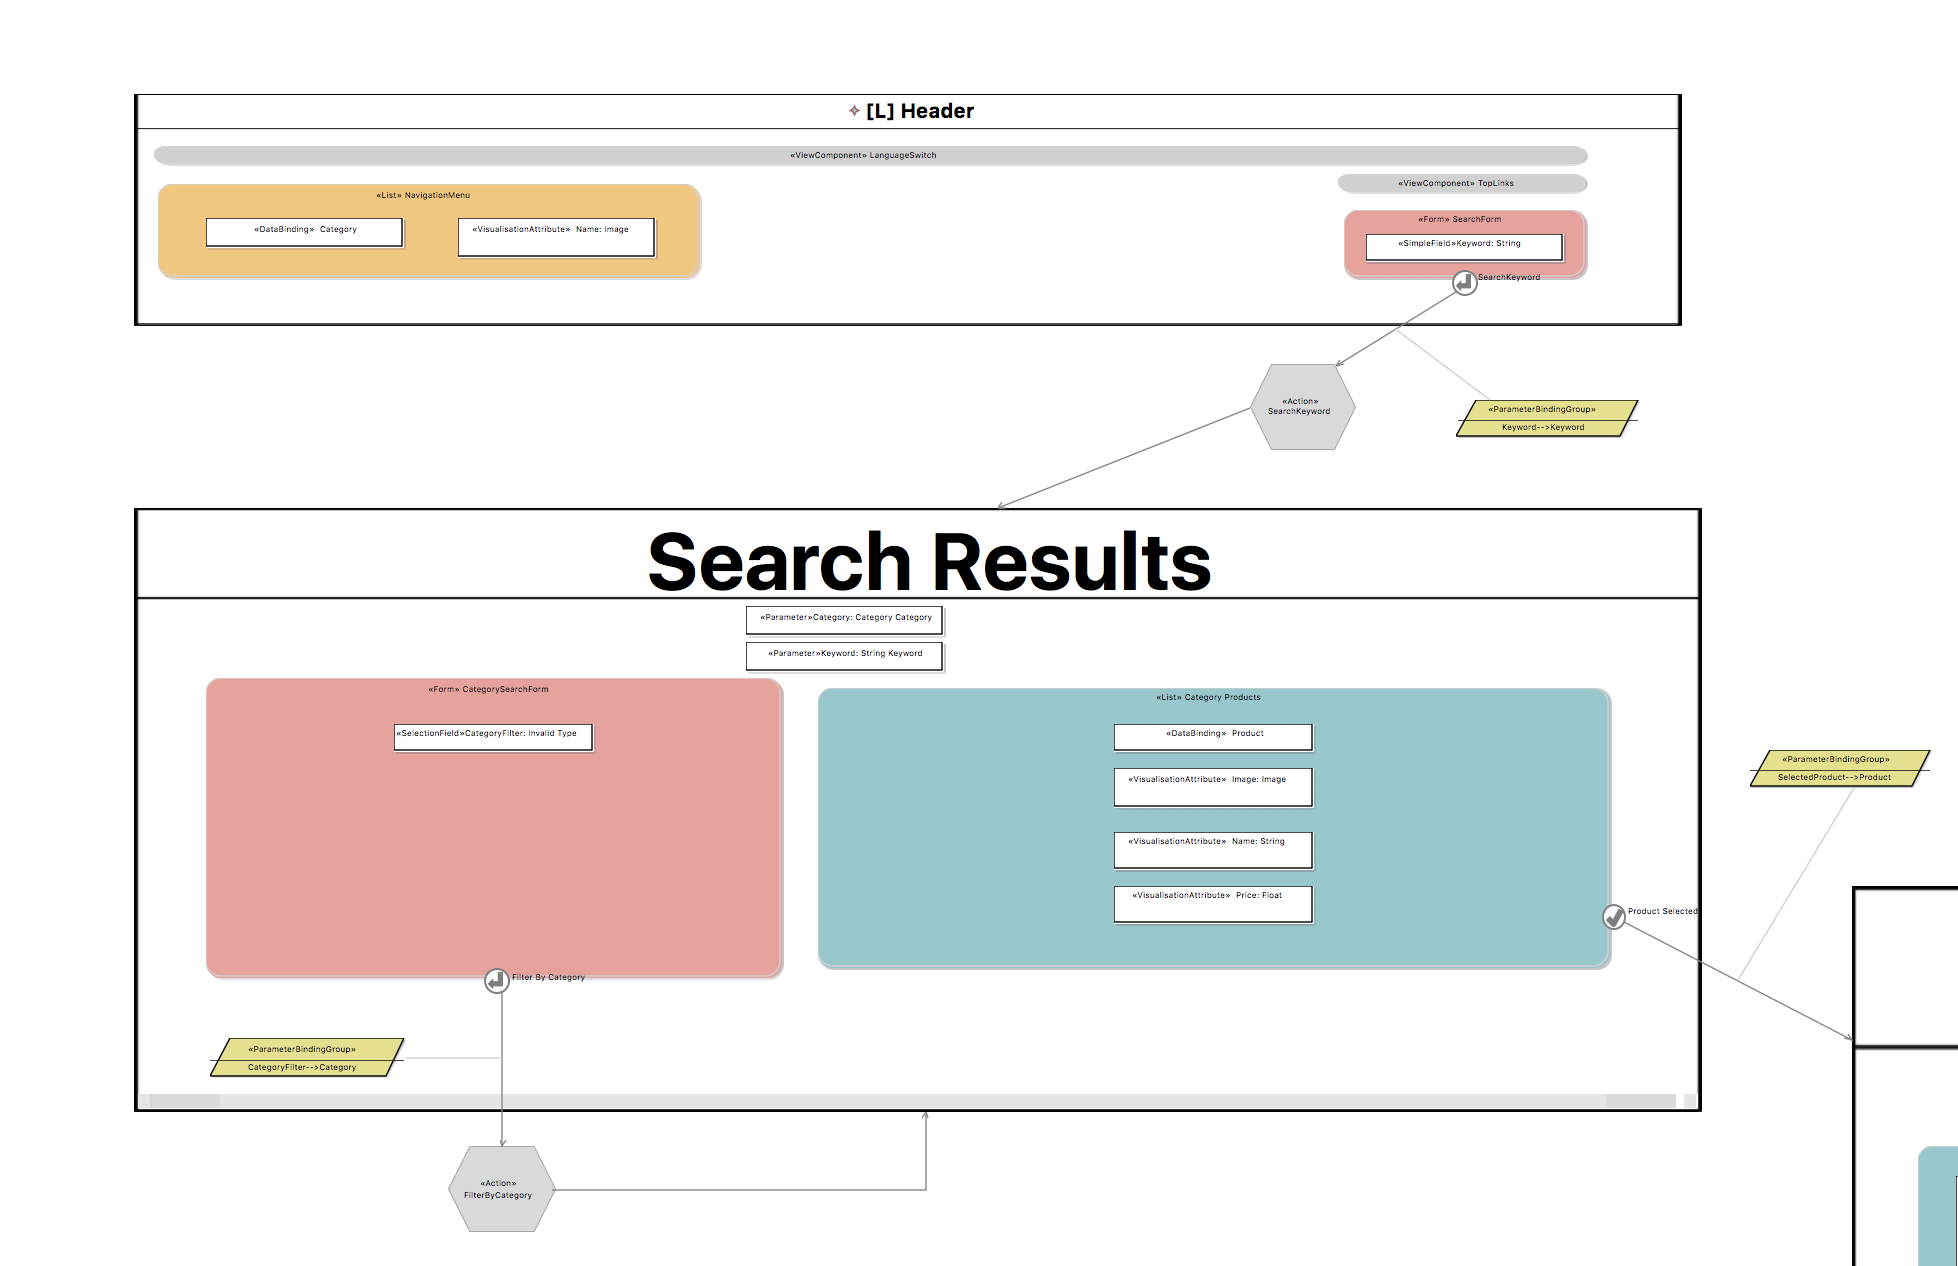
\includegraphics[width=12cm]{images/diagrams/before/ifml-header-search.png}
  \caption{Header and Search sections IFML Diagrams}
  \label{fig:ifml-before-header-search}
\end{figure}
\vspace{0.5cm}

The Footer \textit{IFMLWindow} model is quite straightforward. It retains the information about the footer links presented on the bottom of all the pages of the website in the form of a simple \textit{ViewComponent} and a Newsletter subscription \textit{Form View Component} reacting to SubscribeNewsletter submit \textit{Events}. Similarly to the header case we have just described, the email passed as an argument from the \textit{Event} is carried to the \textit{IFMLAction} which, in this specific case, performs the actual Customer subscription and redirects them to the current page.(Figure \ref{fig:ifml-before-footer}).

\vspace{0.5cm}
\begin{figure}[H]
  \centering
    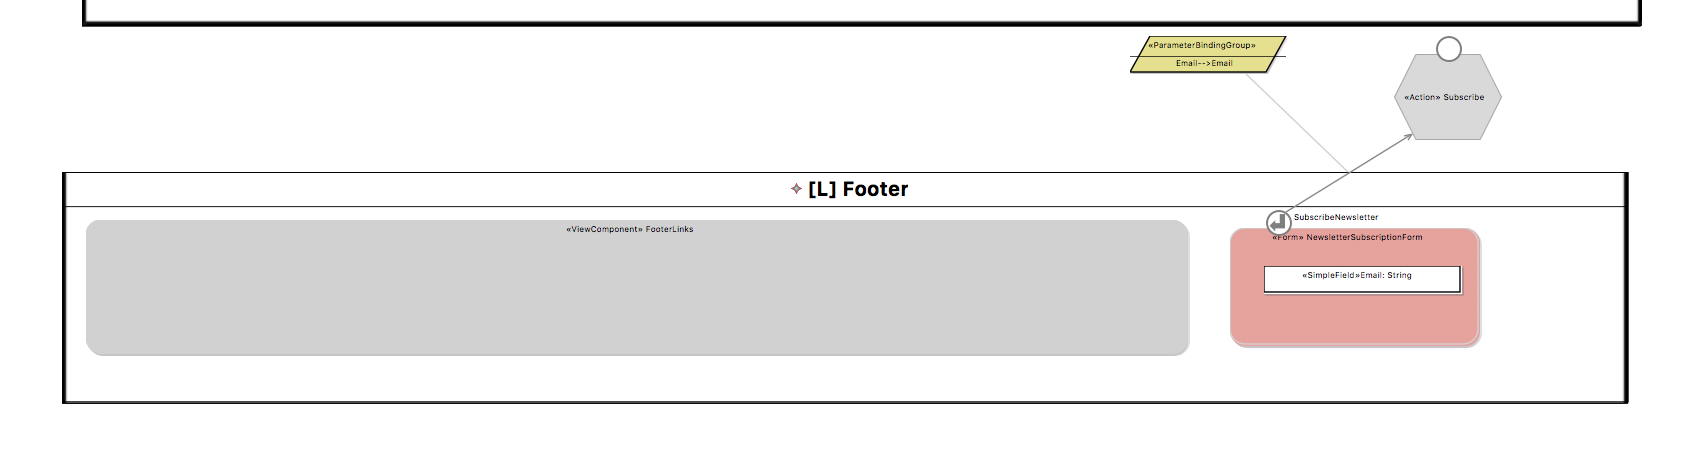
\includegraphics[width=12cm]{images/diagrams/before/ifml-footer.png}
  \caption{Footer section IFML Diagram}
  \label{fig:ifml-before-footer}
\end{figure}
\vspace{0.5cm}

\newpage
We conclude this chapter with both a snippet of the Header \textit{IFMLWindow} element code coming from the \textit{IFMLModel}, and an excerpt of the eCore diagram for the areas of the website we described in this subsection (Figure \ref{fig:ifml-before-hierarchy-headersearchfooter}).

\vspace{0.5cm}
\lstset{language=XML}
\begin{lstlisting} 
  <interactionFlowModelElements xsi:type="ext:IFMLWindow" id="_LvuL0BPREei3TrqMA9Bdvw" name="Header" isLandmark="true">
  <viewElements xsi:type="ext:List" id="_v0p5YA9BEeiZ14TmPBeBNA" name="NavigationMenu">
    <viewComponentParts xsi:type="core:DataBinding" id="__mcXIA9BEeiZ14TmPBeBNA" name="Category"/>
    <viewComponentParts xsi:type="core:VisualizationAttribute" id="_Kbzt3xIZEeijSslFDgCgZA" name="Name" featureConcept="//@domainModel/@domainElements.5"/>
  </viewElements>
  <viewElements xsi:type="ext:Form" id="_YWvrMA9GEeiZ14TmPBeBNA" name="SearchForm">
    <viewElementEvents xsi:type="ext:OnSubmitEvent" id="_ULm7WRIWEeijSslFDgCgZA" name="SearchKeyword" viewElement="//@interactionFlowModel/@interactionFlowModelElements.4/@viewElements.1">
      <outInteractionFlows xsi:type="core:NavigationFlow" id="_Y6uV1xIWEeijSslFDgCgZA" targetInteractionFlowElement="//@interactionFlowModel/@interactionFlowModelElements.3">
        <parameterBindingGroup id="_yCY84hPOEei3TrqMA9Bdvw">
          <parameterBindings id="_y5vbohPOEei3TrqMA9Bdvw" sourceParameter="//@interactionFlowModel/@interactionFlowModelElements.4/@viewElements.1/@viewComponentParts.0" targetParameter="//@interactionFlowModel/@interactionFlowModelElements.3/@parameters.0"/>
        </parameterBindingGroup>
      </outInteractionFlows>
    </viewElementEvents>
    <viewComponentParts xsi:type="ext:SimpleField" id="_lWoCAA9GEeiZ14TmPBeBNA" name="Keyword" direction="out" />
  </viewElements>
  <viewElements xsi:type="core:ViewComponent" id="_aQFfjQ9TEeiZ14TmPBeBNA" name="TopLinks"/>
  <viewElements xsi:type="core:ViewComponent" id="_ezXdfQ9TEeiZ14TmPBeBNA" name="LanguageSwitch"/>
</interactionFlowModelElements>
\end{lstlisting}
\vspace{0.5cm}


\vspace{0.5cm}
\begin{figure}[H]
  \centering
    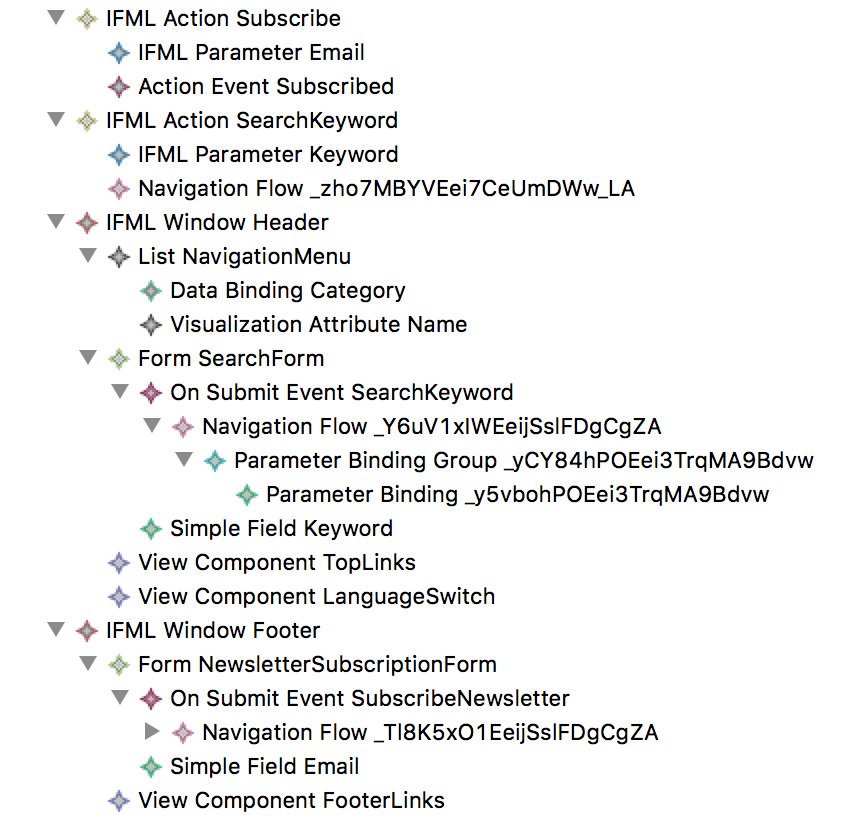
\includegraphics[width=12cm]{images/diagrams/before/ifml-hierarchy-headersearchfooter.png}
  \caption{Interaction Flow for the shared elements in EMF}
  \label{fig:ifml-before-hierarchy-headersearchfooter}
\end{figure}
\vspace{0.5cm}


\clearpage

 % !TEX root = Tesi.tex
\chead{}

\chapter{Enhancing web models via model transformations}
\label{enhancing-web-models-via-model-transformations}

In the previous chapter, after describing both metamodels for the Real Usage Data and the Interaction Flow Modeling Language, we proceeded with creating dynamic instances for both models, respectively describing the actual input data available for the customisation process and the initial \textit{IFMLModel} of the eCommerce Madison Island website. In this chapter, we illustrate a possible transformation for this model, based on the Real Usage instance data. Our goal is to upgrade the model version, taking into account customers preferences and their actions.


\section{Refactoring Actions}

In this section, we explain how each \textit{IFMLWindow} container of the starting website \textit{IFMLModel} can be potentially upgraded accordingly to the Real Usage Data model described in the previous chapter.

\subsection{Homepage}
\label{homepage-updates}

Considering the data coming from the Proximity sensors within the actual Madison Island retail store, we are aware of a set of regions corresponding to the customer preferred categories. That information will be used to change the content and, therefore, the \textit{IFMLModel} for the Homepage carousel.

For instance, we know that the \textbf{Blazers}, \textbf{Tees, Knits and Polos} and \textbf{Shoes} categories correspond to the \textit{sessionRegion} elements within the store in which the user spent more time after sorting the entries by \textit{maxSecondsInRegion} and \textit{maxProximity} attributes. In the case of the Blazers category for example, the data belonging to the \textit{RealUsageData:ProximityData} parent node takes this form:

\vspace{0.5cm}
\lstset{language=XML}
\begin{lstlisting} 
  <sessionRegions
  regionId="40"
  regionLabel="blazers"
  detectionCount="1"
  maxSecondsInRegion="195"
  maxProximity="immediate"
  firstDetectionTimeStamp="2018-02-21T18:11:01.000+0100"
  lastDetectionTimeStamp="2018-02-21T18:11:01.000+0100">
  <beaconData
    uuid="0686a88e-fed6-11e7-8be5-0ed5f89f718b"
    majorId="25911"
    minorId="27"/>
</sessionRegions>
\end{lstlisting}
\vspace{0.5cm}

By applying this knowledge, we can say that the \textit{subViewComponentParts} and the \textit{parameter} nodes of the first HightlightedCategoriesCarousel \textit{IFMLWindow} elements from the initial \textit{IFMLModel} can be modified from this:

\vspace{0.5cm}
\lstset{language=XML}
\begin{lstlisting} 
<parameters  name="Highlighted Category #1" direction="inout">
  <constraints  language="SQL" body="Category.ID=18"/>
</parameters>

...

<subViewComponentParts xsi:type="core:ConditionalExpression"  language="SQL" body="Category.ID=18" name="Eyewear"/>
\end{lstlisting}
\vspace{0.5cm}

to:

\vspace{0.5cm}
\lstset{language=XML}
\begin{lstlisting} 
  <parameters  name="Highlighted Category #1" direction="inout">
  <constraints  language="SQL" body="Category.ID=40"/>
</parameters>

...

<subViewComponentParts xsi:type="core:ConditionalExpression"  language="SQL" body="Category.ID=40" name="Blazers"/>
\end{lstlisting}
\vspace{0.5cm}

Besides updating the content by prioritising some categories, the \textit{IFMLModel} can also be changed to use different IFML elements under certain conditions. For example, the \textit{List View Component}, which is responsible for displaying the most recent products on the homepage, can be replaced by another \textit{List View Component}, responsible for presenting the latest products with which customers interacted in the physical store. Information about these products is available in the RealUsageData model under the \textit{RealUsageData:ActionData} section. In our specific example, \textit{RealUsageData:ActionData} contains the data about the product SKUs that the customer had scanned for collecting reward points.

\vspace{0.5cm}
\lstset{language=XML}
\begin{lstlisting} 
<sessionActions userAgent="iPhone 6S">
  <scannedItems 
  barcode="042100005264" name="Elizabeth Knit Top-Red-S" sku="wbk012c-Red-S"/>
  <scannedItems 
  barcode="042100005931" name="Plaid Cotton Shirt-Khaki-L" sku="msj006c-Khaki-L"/>
  <scannedItems 
  barcode="042100007717" name="Broad St Saddle Shoes" sku="shm00110"/>
</sessionActions>
\end{lstlisting}
\vspace{0.5cm}


The model transition in this case would occur not only replacing the IFML \textit{View Component} with a different type, but also adding a \textit{ConditionalExpression} that filters the items by their SKUs, as shown in Figure \ref{fig:ifml-transformation-example}.

\vspace{0.5cm}
\begin{figure}[H]
  \centering
    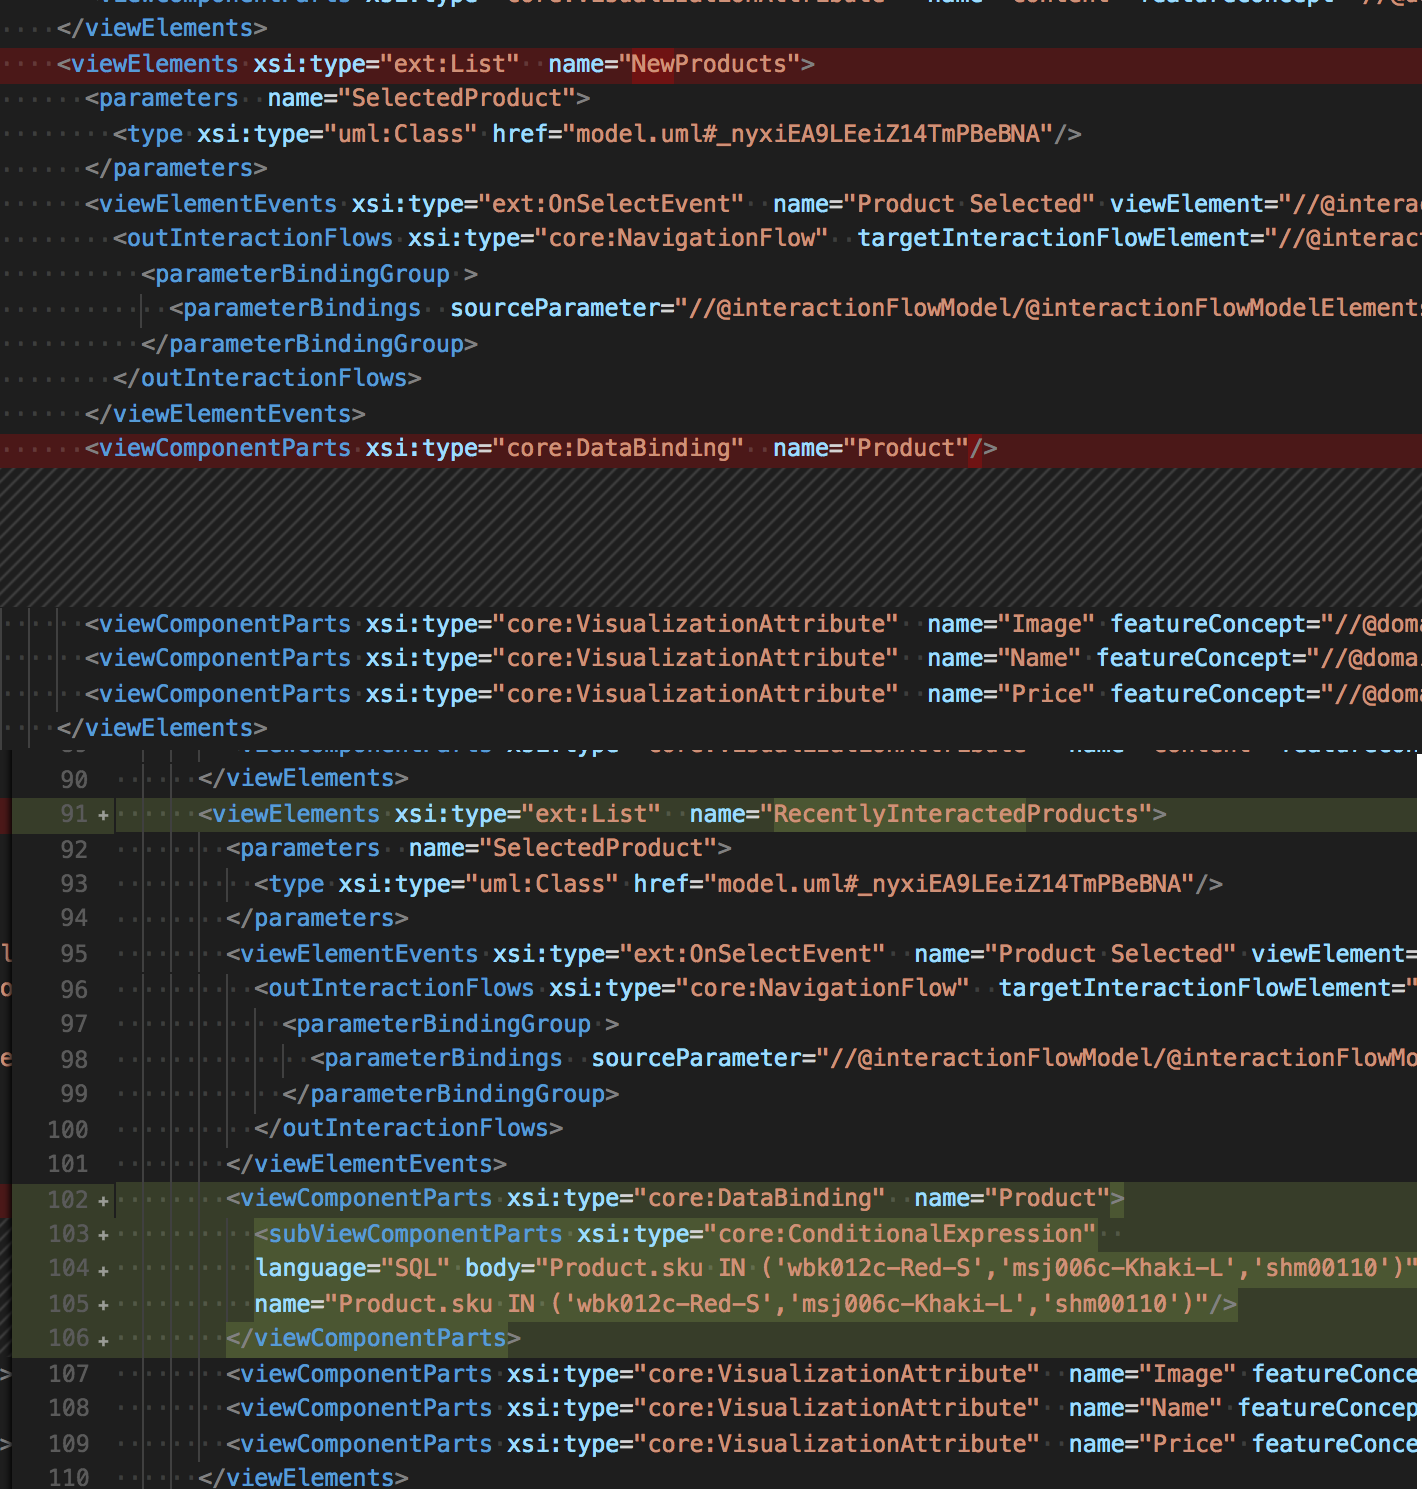
\includegraphics[height=10cm]{images/madison/ifm-homepage-transformation.png}
  \caption{IFML Homepage transformation example}
  \label{fig:ifml-transformation-example}
\end{figure}
\vspace{0.5cm}

\subsection{Header}
\label{header-updates}

Leveraging once more the \textit{RealUsageData:ActionData}, the Header node of the \textit{IFMLModel} describing the top area in the Madison Island website could also be enhanced to show a list of recent actions performed by customers in the physical stores that generated reward points.  This can be achieved by appending an instance of \textit{List View Component} to the \textit{interactionFlowModelElements} parent node, called \textit{RecentRewardActions}. This instance is then linked to the Rewards \textit{Data Binding} entity, which allows the visualization of the \textit{Action Name} and \textit{Points Attribution} properties to the front-end, as shown in the following snippet of \textit{IFMLModel} code:

\vspace{0.5cm}
\lstset{language=XML}
\begin{lstlisting} 
  <interactionFlowModelElements xsi:type="ext:IFMLWindow"  name="Header" isLandmark="true">
  <viewElements xsi:type="ext:List"  name="NavigationMenu">
   ...
  </viewElements>
  <viewElements xsi:type="ext:Form"  name="SearchForm">
   ...
  </viewElements>
  <viewElements xsi:type="core:ViewComponent"  name="TopLinks"/>
  <viewElements xsi:type="core:ViewComponent"  name="LanguageSwitch"/>

  <!-- ADDED NODE -->
  <viewElements xsi:type="ext:List"  name="RecentRewardActions">
    <viewComponentParts xsi:type="core:DataBinding"  name="Rewards" domainConcept="//@domainModel/@domainElements.13"/>
    <viewComponentParts xsi:type="core:VisualizationAttribute"  name="Action Name" featureConcept="//@domainModel/@domainElements.15"/>
    <viewComponentParts xsi:type="core:VisualizationAttribute"  name="Points Attribution" featureConcept="//@domainModel/@domainElements.14"/>
  </viewElements>
  <!-- ADDED NODE -->

  </interactionFlowModelElements>

  <domainModel name="MadisonIsland">
   ....
   <!-- ADDED NODES -->
    <domainElements xsi:type="core:UMLDomainConcept" name="Rewards" dataBinding="//@interactionFlowModel/@interactionFlowModelElements.4/@viewElements.4/@viewComponentParts.0"/>
    <domainElements xsi:type="core:UMLStructuralFeature"  name="RewardPoints" visualizationAttribute="//@interactionFlowModel/@interactionFlowModelElements.4/@viewElements.4/@viewComponentParts.2"></domainElements>
    <domainElements xsi:type="core:UMLStructuralFeature"  name="RewardName">
    </domainElements>
   <!-- ADDED NODES -->
   ...
 </domainModel>
\end{lstlisting}
\vspace{0.5cm}

Additionally, since we are introducing references to new \textit{domainElements} nodes linked to the added \textit{viewComponentParts} children nodes, they must be appended to the \textit{domainModel} node as part of the transformation.

\subsection{Category Page}
\label{category-page-updates}

In light of the information gathered in the Real Usage Data model about the recently viewed products available in the \textit{RealUsageData:WebData} node, the Category page can be enhanced by appending an additional visual element to the user interface for tracking that information.

To do so, we filter out the RealUsageData model, fetching the nodes containing a \textit{parameterBindingGroup} property and including a Product reference like the following entries:

\vspace{0.5cm}
\lstset{language=XML}
\begin{lstlisting} 
      <data xsi:type="RealUsageData:WebData"
      ID="3"
      name="AccessLog"
      userID="3045678"
      date="2017-11-29T07:08:40.000+0100"
      viewContainer="Category #15"
      viewComponent="ProductList"
      eventType="click"
      parameterBindingGroup="Product/404"
      logEntry="GET /men/shirts/plaid-cotton-shirt-476.html 200 0 - 29505"/>
      
      <data xsi:type="RealUsageData:WebData"
      ID="4"
      name="AccessLog"
      userID="3045678"
      date="2017-12-04T06:37:15.000+0100"
      viewContainer="Product #404"
      viewComponent="RelatedProductList"
      eventType="click"
      parameterBindingGroup="Product/413"
      logEntry="GET /core-striped-sport-shirt-551.html 200 0 - 29505"/>

      <data xsi:type="RealUsageData:WebData"
      ID="8"
      name="AccessLog"
      userID="3045678"
      date="2017-12-04T06:38:20.000+0100"
      viewContainer="Search Results"
      viewComponent="ProductList"
      eventType="click"
      parameterBindingGroup="Product/407"
      logEntry="GET /stretch-cotton-blazer-587.html 200 0 - 29505"/>
\end{lstlisting}
\vspace{0.5cm}

With the data described above, we can then proceed with transforming the initial \textit{IFMLModel} for the Category page, appending to it a \textit{RecentlyViewedProducts} section in the form of a \textit{List View Component} bound to the Product \textit{Data Binding} entity.

This new IFML item would be responsible for presenting customers with the thumbnails, names, and prices of these products, separating them through a distinct \textit{ConditionalExpression}. That expression maps the children node of the \textit{RealUsageData:WebData} dataset shown previously, before finally returning the items in the order they were browsed, and regardless of the display mode property of the Category itself (Figure \ref{fig:recently-viewed-ifml-definition}).

\vspace{0.5cm}
\begin{figure}[H]
  \centering
    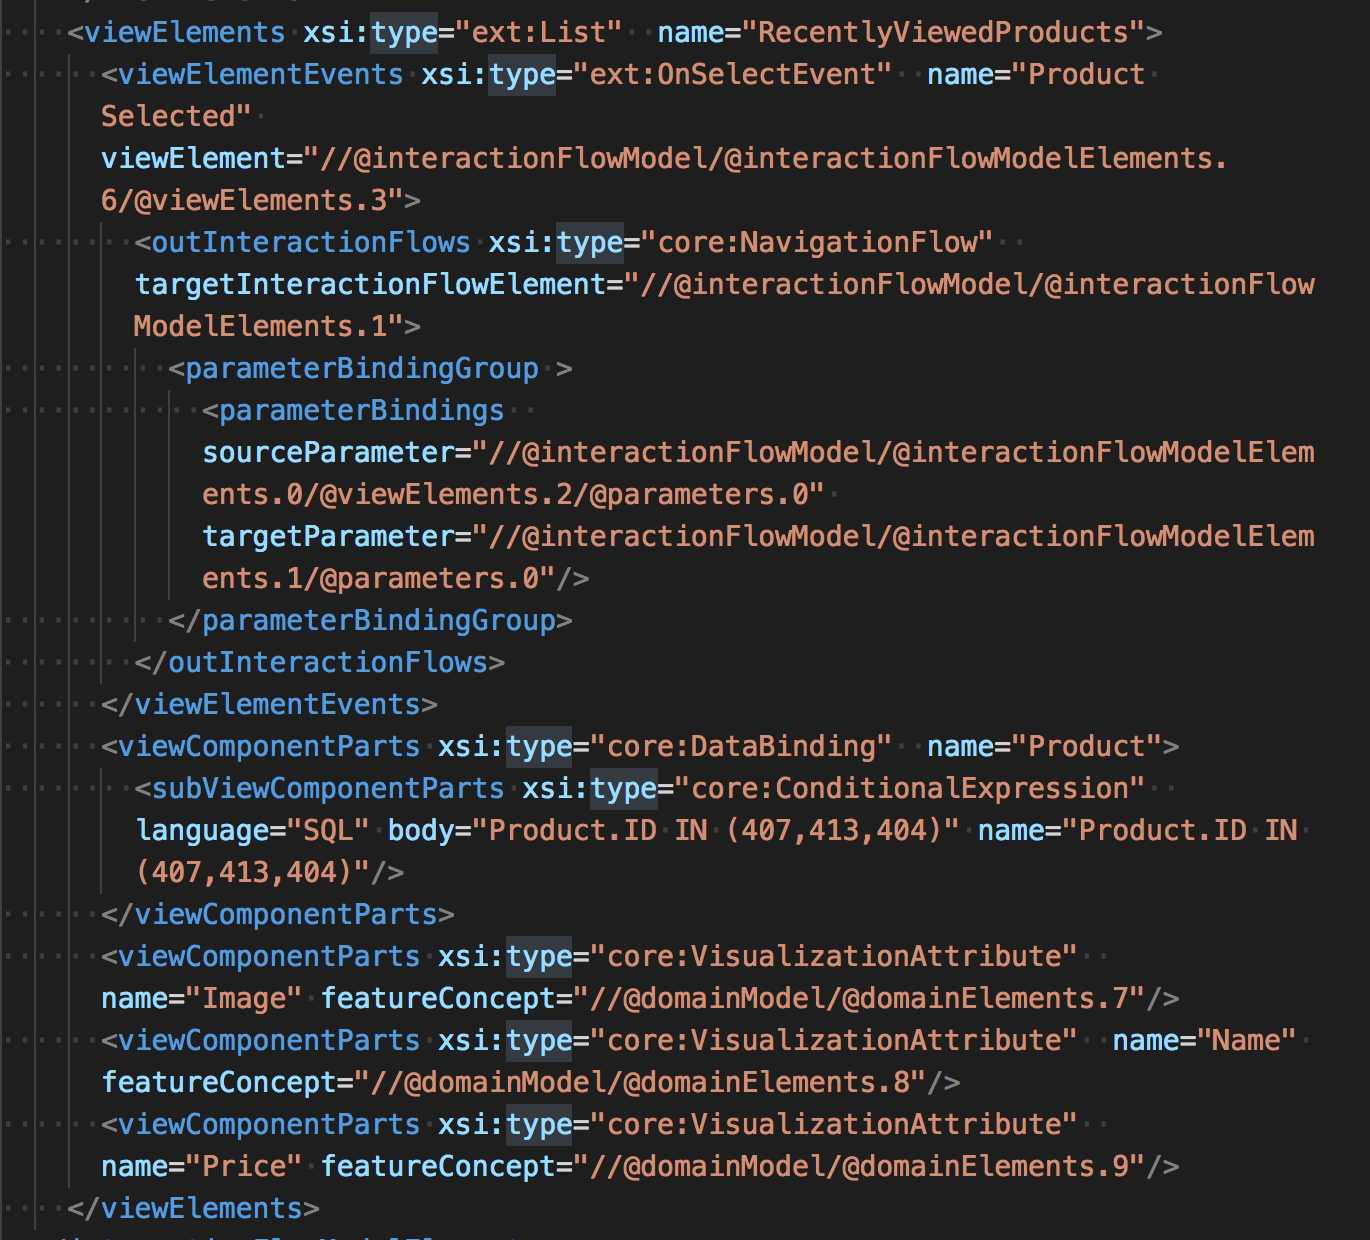
\includegraphics[height=10cm]{images/madison/ifml-recently-viewed.png}
  \caption{Recently Viewed IFML definition snippet}
  \label{fig:recently-viewed-ifml-definition}
\end{figure}
\vspace{0.5cm}

\subsection{Product Page}
\label{product-page-updates}

As far as the possible improvements on the product page of the Madison Island website are concerned, we concentrated on the Related Products widget shown below the Add To Cart section. In the first \textit{IFMLModel}, the list of products related to the currently shown item has no particular assigned logic. Our potential transformation is to extend the \textit{viewElements} node of the \textit{IFMLModel}, taking into account users browsing patterns that have been identified by examining the RealUsageData instances entries.

For example, we could have discovered that, during a same recorded sessions, the \textbf{Core Striped Sport Shirt} and the \textbf{Plaid Cotton Shirt} product pages are frequently browsed together. That could be done by analysing the values set in the \textit{viewContainer}, \textit{viewComponent}, and \textit{parameterBindingGroup} properties for the nodes belonging to the \textit{RealUsageData:WebData} dataset. Such change allows us to take advantage of this correlation, pushing specific products on the Related Products section and consequently offering a more tailored user experience.

The change on the starting \textit{IFMLModel} that would occur in that case restricts the \textit{Data Binding} scope, appending a \textit{subViewComponentParts} to it. That change limits the products collection to the computed set of related products SKUs. The additional \textit{ConditionalExpression} would also be bound to a specific \textit{ActivationExpression}, which would enable the above mentioned filtering only when a customised collection is available for the current product. 

From a \textit{IFMLModel} code perspective, we would transition from the following node configuration for the \textit{List View Component} that controls the Related Product widget:

\vspace{0.5cm}
\lstset{language=XML}
\begin{lstlisting} 
  <viewElements xsi:type="ext:List"  name="RelatedProductList">
  <viewElementEvents xsi:type="ext:OnSelectEvent"  name="Product Selected" viewElement="//@interactionFlowModel/@interactionFlowModelElements.1/@viewElements.2">
    ...
  </viewElementEvents>
  <viewComponentParts xsi:type="core:DataBinding"  name="Product"/>
  <viewComponentParts xsi:type="core:VisualizationAttribute"  name="Image" featureConcept="//@domainModel/@domainElements.7"/>
  <viewComponentParts xsi:type="core:VisualizationAttribute"  name="Name" featureConcept="//@domainModel/@domainElements.8"/>
  <viewComponentParts xsi:type="core:VisualizationAttribute"  name="Price" featureConcept="//@domainModel/@domainElements.9"/>
</viewElements>
\end{lstlisting}
\vspace{0.5cm}

\newpage
to this one:

\vspace{0.5cm}
\lstset{language=XML}
\begin{lstlisting} 
  <viewElements xsi:type="ext:List"  name="RelatedProductList">
  <viewElementEvents xsi:type="ext:OnSelectEvent"  name="Product Selected" viewElement="//@interactionFlowModel/@interactionFlowModelElements.1/@viewElements.2">
      ...
  </viewElementEvents>
  <viewComponentParts xsi:type="core:DataBinding"  name="Product">
    <subViewComponentParts xsi:type="core:ConditionalExpression"  language="SQL" body="Product.ID IN getCustomizedRelatedProducts()" name="Product.ID IN getCustomizedRelatedProducts" activationExpression="//@interactionFlowModel/@interactionFlowModelElements.17"/>
  </viewComponentParts>
  <viewComponentParts xsi:type="core:VisualizationAttribute"  name="Image" featureConcept="//@domainModel/@domainElements.7"/>
  <viewComponentParts xsi:type="core:VisualizationAttribute"  name="Name" featureConcept="//@domainModel/@domainElements.8"/>
  <viewComponentParts xsi:type="core:VisualizationAttribute"  name="Price" featureConcept="//@domainModel/@domainElements.9"/>
</viewElements>
\end{lstlisting}
\vspace{0.5cm}

Moreover, the \textit{ActivationExpression} defined by the \textit{interactionFlowModelElements} XPath expression presented above links to a node responsible for controlling the feature with the following content:

\vspace{0.5cm}
\lstset{language=XML}
\begin{lstlisting} 
<interactionFlowModelElements 
  xsi:type="core:ActivationExpression" id="CurrentProduct.hasCustomizedRelatedProduct" language="SQL" body="CurrentProduct.hasCustomizedRelatedProduct()">
</interactionFlowModelElements>

\end{lstlisting}
\newpage
\vspace{0.5cm}
\subsection{Shopping Cart}
\label{shopping-cart-updates}

As described in \ref{shopping-cart-page-overview}, the Shopping Cart page model includes two main sections. The first is a \textit{List Product List} component, responsible for the interactions with the cart items. The second is the \textit{IFMLWindow}, used for grouping the actions triggered by customers when they apply discounts or estimate shipping and taxes for their current quote.

\vspace{0.5cm}
\begin{figure}[H]
  \centering
    \includegraphics[width=12cm]{images/madison/ifml-shopping-cart-sidebar.png}
  \caption{Shopping Cart Sidebar IFML definition snippet}
  \label{fig:shopping-cart-sidebar-ifml-definition}
\end{figure}
\vspace{0.5cm}

Along with the cases analysed previously and by applying the data from the Real Data Usage model, we can modify and extend the interaction flow of this page by adding a new \textit{View Component}. That component shows the Reward points accumulated by the user in the Shopping Cart Sidebar (Figure \ref{fig:shopping-cart-sidebar-ifml-definition}). The component not only displays the information by the \textit{Data Binding} with the Reward entity, but also controls the \textit{Event} associated with the \textbf{``Apply Discount"} button and the \textit{Action} connected to it. 
The structure of this new node, which gets appended to its parent \textit{IFMLMenu}, is as follows:

\vspace{0.5cm}
\lstset{language=XML}
\begin{lstlisting} 
  <viewElements xsi:type="core:ViewComponent" name="Applicable Reward Points">
    <viewElementEvents xsi:type="ext:OnSelectEvent" name="Apply Reward Points" viewElement="//@interactionFlowModel/@interactionFlowModelElements.11/@viewElements.2/@viewElements.3">
        <outInteractionFlows xsi:type="core:NavigationFlow" targetInteractionFlowElement="//@interactionFlowModel/@interactionFlowModelElements.18/@actionEvents.0"/>
    </viewElementEvents>
    <viewComponentParts xsi:type="core:DataBinding" name="Reward"/>
    <viewComponentParts xsi:type="core:VisualizationAttribute"  name="Available Reward Points" featureConcept="//@domainModel/@domainElements.14"/>
</viewElements>
\end{lstlisting}
\vspace{0.5cm}

\newpage
\section{The \textit{IFMLRUD2IFML} Model Transformation}

In this section, we illustrate the model-to-model transformation that allows to update web models according to the above described refactoring actions. A fragment of the \textit{IFMLRUD2IFML} transformation implemented in ATL\cite{ATL} is depicted in Listing~\ref{lst:IFMLRUD2IFML}. It takes as input two models, \textit{IN}
conforms to the IFML metamodel and  \textit{IN2} conforms to the Real Usage Data (RUD) metamodel, and generate an \textit{OUT} model conforms to the IFML metamodel. The listing contains the following rules: 

\begin{itemize}
	\item[-] The rule \textit{ConditionalExpressionUpdated} matches the element of type \textit{ConditionalExpression} named \textit{``HighlightedCategoryBanner \#1"} and modifies its name and category. To this end, the helper \textit{getMaxSecondsInRegion()} is used to get the element of type \textit{SessionRegion} belonging to the RUD model that has the higher value of seconds in region among the ones having \textit{maxSecondsInRegion} greater than 100.

	\item[-] The rule \textit{IFMLWindow} matches the element of type \textit{IFMLWindow} and modifies it as follows: 
\begin{itemize}
	\item[-] if the element is named \textit{``Header"} and the helper \textit{hasSectionActions()} (that verify if the element of type \textit{SectionAction} contains at least one element of type \textit{ScannedItems}) is true, then the new elements defined in the rule \textit{RecentRewardActions()} are added; 
	\item[-] if the element is named \textit{``Category"} and the helper \textit{hasWebData()} (that verify if the element of type \textit{WebData} contains a  \textit{parameterBindingGroup}) is true, then the new elements defined in the rule \textit{RecentViewedProducts()} are added; 
\end{itemize} 
\end{itemize}

Such rules implement the refactoring actions illustrated in Sections \ref{homepage-updates}, \ref{header-updates} and \ref{category-page-updates}.
\vspace{0.5cm}

\begin{lstlisting}[breaklines,style=AMMA,language=ATL,mathescape,rulesepcolor=\color{black},caption={ A fragment of the transformation},captionpos=b, aboveskip=0.2cm, belowskip=0cm, label={lst:IFMLRUD2IFML}]
module IFMLRUD2IFML;

create OUT : IFML from IN : IFML, IN2: RUD;

helper def : inElements : Set(IFML!"ecore::EObject") = 		
	IFML!"ecore::EObject".allInstancesFrom('IN');

-- getMaxSecondsInRegion()
helper def : getMaxSecondsInRegion() : RUD!SessionRegion = 
	RUD!SessionRegion.allInstancesFrom('IN2')->select(e|e.maxSecondsInRegion > 100).first();

-- hasSectionActions()
helper def : hasSectionActions() : Boolean = 
	RUD!SessionAction.allInstancesFrom('IN2')->select(e|e.scannedItems->notEmpty())->notEmpty();

-- hasWebData()
helper def : hasWebData() : Boolean = 
	RUD!WebData.allInstancesFrom('IN2')->select(e| not e.parameterBindingGroup->oclIsUndefined())->notEmpty();
...
-- Homepage Refactoring
rule ConditionalExpressionUpdated {
	from s : IFML!"IFML::Core::ConditionalExpression" 		
		(thisModule.inElements->includes(s) 
		and s->refImmediateComposite()->refImmediateComposite()->refImmediateComposite().name = 'HighlightedCategoryBanner #1')
	to t : IFML!"IFML::Core::ConditionalExpression" (
		__xmiID__ <- s.__xmiID__,
		id <- s.id,
		language <- s.language,
		body <- s.body,
		constraints <- s.constraints,
		annotations <- s.annotations,
		parameters <- s.parameters,
		outInteractionFlows <- s.outInteractionFlows,
		inInteractionFlows <- s.inInteractionFlows,
		viewElementEvents <- s.viewElementEvents,
		activationExpression <- s.activationExpression,
		subViewComponentParts <- s.subViewComponentParts)
	do {
		t.name <- thisModule.getMaxSecondsInRegion().regionLabel;
		t.body <- 'Category.ID=' + thisModule.getMaxSecondsInRegion().regionId;
	}
}
....
-- Header Refactoring + Category Page Refactoring
rule IFMLWindow {
	from s : IFML!"IFML::Extensions::IFMLWindow" 	
		(thisModule.inElements->includes(s))
	to t : IFML!"IFML::Extensions::IFMLWindow" (
		__xmiID__ <- s.__xmiID__,
		id <- s.id,
		name <- s.name,
		isLandmark <- s.isLandmark,
		isDefault <- s.isDefault,
		isXOR <- s.isXOR,
		isModal <- s.isModal,
		isNewWindow <- s.isNewWindow,
		constraints <- s.constraints,
		annotations <- s.annotations,
		parameters <- s.parameters,
		outInteractionFlows <- s.outInteractionFlows,
		inInteractionFlows <- s.inInteractionFlows,
		viewElementEvents <- s.viewElementEvents,
		activationExpression <- s.activationExpression,
		viewElements <- s.viewElements,
		actions <- s.actions)
	do {
		if (s.name = 'Header' and thisModule.hasSectionActions()) {
			t.viewElements <- thisModule.RecentRewardActions();
		} 
		if (s.name = 'Category' and thisModule.hasWebData()){
			t.viewElements <- thisModule.RecentViewedProducts();
		}
	}		
}

-- create an additional node to header
rule RecentRewardActions() {
	to v : IFML!"IFML::Extensions::List" (
		name <- 'RecentRewardActions',
		viewComponentParts <- Sequence{w,y,z}
	),
	w : IFML!"IFML::Core::DataBinding" (
		name <- 'Rewards'
	),
	y : IFML!"IFML::Core::VisualizationAttribute" (
		name <- 'Action Name'
	),
	z : IFML!"IFML::Core::VisualizationAttribute" (
		name <- 'Points Attribution'
	)
	do {
		v;
	}
}

-- create an additional node to category page
rule RecentViewedProducts() {
	to v : IFML!"IFML::Extensions::List" (
		name <- 'RecentlyViewedProducts',
		viewComponentParts <- Sequence{w,y,z1,z2,z3}
	),
	w : IFML!"IFML::Extensions::OnSelectEvent" (
		name <- 'Product Selected'
	),
	y : IFML!"IFML::Core::DataBinding" (
		name <- 'Product'
	),
	z1 : IFML!"IFML::Core::VisualizationAttribute" (
		name <- 'Image'
	),
	z2 : IFML!"IFML::Core::VisualizationAttribute" (
		name <- 'Name'
	),
	z3 : IFML!"IFML::Core::VisualizationAttribute" (
		name <- 'Price'
	)
	do {
		v;
	}
}
.....
\end{lstlisting}
\vspace{0.5cm}


\newpage
\section{Updated web models}

In this section, we present an overview of the updated \textit{IFMLModel}s for the Madison Island website based on the transformations discussed in the last chapter. We also describe how their IFMLDiagrams and corresponding website front-end screens would look like.

\subsection{Homepage}

According to what we described in \ref{homepage-updates}, the enhanced homepage presented to the customer would show a custom banner carousel and a product widget, both containing items and categories with which the user interacted in the retail store.

\vspace{0.5cm}
\begin{figure}[H]
  \centering
    \includegraphics[width=16cm]{images/diagrams/after/ifml-homepage.png}
  \caption{Updated Homepage IFML Diagram}
  \label{fig:ifml-after-homepage}
\end{figure}

\begin{figure}[H]
  \centering
    \includegraphics[width=16cm]{images/diagrams/after/desktop-homepage.png}
  \caption{Updated Homepage Desktop}
  \label{fig:desktop-after-homepage}
\end{figure}
\vspace{0.5cm}

\newpage
\subsection{Header}

After transforming its \textit{IFMLModel} component (\ref{header-updates}), the shared header section on the website reveals new information through a new widget. This widget is aligned on the right side of the area used for advertising the actions taken by the user in the retail store and their respective rewarded points.

\vspace{0.5cm}
\begin{figure}[H]
  \centering
    \includegraphics[width=14cm]{images/diagrams/after/ifml-header.png}
  \caption{Updated Header IFML Diagram}
  \label{fig:ifml-after-header}
\end{figure}

\begin{figure}[H]
  \centering
    \includegraphics[width=14cm]{images/diagrams/after/desktop-header.png}
  \caption{Updated Header Desktop Version}
  \label{fig:desktop-after-header}
\end{figure}
\vspace{0.5cm}

\newpage
\subsection{Category Page}

Regardless of the DisplayMode property set for each Category Page on the eCommerce platform, the updated web model presents a vertical section on the right sidebar. That section maps the URLs browsed recently in a same user session that have been identified during the model transformation phase (\ref{category-page-updates}).

\vspace{0.5cm}
\begin{figure}[H]
  \centering
    \includegraphics[width=14cm]{images/diagrams/after/ifml-category.png}
  \caption{Updated Category Page IFML Diagram}
  \label{fig:ifml-after-category}
\end{figure}

\begin{figure}[H]
  \centering
    \includegraphics[width=14cm]{images/diagrams/after/desktop-category.png}
  \caption{Updated Category Page Desktop Version}
  \label{fig:desktop-after-category}
\end{figure}
\vspace{0.5cm}

\newpage
\subsection{Product Page}

Differently from the other page enhancements presented so far, the modified web model for the Product Page does not offer any additional visual segments to the page when compared to its starting \textit{IFMLModel}. As discussed in \ref{product-page-updates}, the change focused on improving the logic behind the related products selection by filtering the items on top of which a browsing correlation was detected. In Figure \ref{fig:desktop-after-product}, we can see an example of this behaviour, where the \textbf{Plaid Cotton Shirt} product is placed as the first one in the Related Products region on the \textbf{Core Striped Sport Shirt} product page.

\vspace{0.5cm}
\begin{figure}[H]
  \centering
    \includegraphics[width=14cm]{images/diagrams/after/ifml-product.png}
  \caption{Updated Product Page IFML Diagram}
  \label{fig:ifml-after-product}
\end{figure}

\begin{figure}[H]
  \centering
    \includegraphics[width=14cm]{images/diagrams/after/desktop-product.png}
  \caption{Updated Product Page Desktop Version}
  \label{fig:desktop-after-product}
\end{figure}
\vspace{0.5cm}

\newpage
\subsection{Shopping Cart}

In \ref{shopping-cart-updates}, we outlined how the visual aspects of the shopping cart sidebar would be transformed through an \textit{IFMLModel} change. This change would result in a new form element within the sidebar, which would be responsible for controlling the application of the reward points available to the customer at that point. Those reward points --- generated through actions recorded as part of the real usage data profiling --- would be converted into discounts that the customer could apply to their current quote at any time. As shown by the attached action in the IFML Diagram, the customer is redirected to the shopping cart page after the discount is applied.

\vspace{0.5cm}
\begin{figure}[H]
  \centering
    \includegraphics[width=14cm]{images/diagrams/after/ifml-shopping-cart.png}
  \caption{Updated Shopping Cart Page IFML Diagram}
  \label{fig:ifml-after-shopping-cart}
\end{figure}

\begin{figure}[H]
  \centering
    \includegraphics[width=14cm]{images/diagrams/after/desktop-shopping-cart.png}
  \caption{Updated Shopping Cart Page Desktop Version}
  \label{fig:desktop-after-shopping-cart}
\end{figure}
\vspace{0.5cm}





%\addcontentsline{toc}{chapter}{}

\clearpage

% !TEX root = Tesi.tex
\chead{}

\chapter{From models to code, a case study.}

This chapter covers a case study based on the applications of the notions previously retrieved describing the Magento platform the Madison Island eCommerce website would run on and proposing a possible automation for code generation compatible with the platform ecosystem and architecture.

\section{Magento overview}

Magento is one of the most powerful and feature-rich online eCommerce platform that was launched on March 31, 2008. 

The platform grants merchants complete flexibility and control over the look, content and functionality of their online store. Thanks to its intuitive administration interface for content management and robust marketing and merchandising tools it gives merchants the ability to create sites that are fully fit their unique business needs, putting no constraints on business processes and flow.

From a technical perspective, the platform incorporates the core architectural principles of an object-oriented, PHP-based application that can be easily used to personalize and expand the existing and already ample out of the box set of features.
In fact, central to the Magento model of software development is the strategy of replacing or extending core code rather than editing it to support maintainability and flexibility. 

To achieve this goal Magento software architecture has been built around the concept of self-contained modules holding discrete code organized by feature, thereby reducing each module’s external dependencies.

The Magento frontend is designed to optimize storefront customization, with highly extensible themes being the central customization mechanism so that merchants can easily extend and transform the appearance of their storefronts.

\vspace{0.5cm}
\begin{figure}[H]
  \centering
    \includegraphics[height=12cm]{images/magento/magento-architecture.jpg}
  \caption{Magento Architecture Overview}
  \label{fig:magento-architecture-overview}
\end{figure}
\vspace{0.5cm}

Interacting with the product and its appearance on a Magento web interface means interacting with presentation layer code composed by both view elements (layouts, blocks, templates) and controllers, which process commands to and from the user interface. 

We can extensively customize this user interface by extending Magento themes capabilities personalizing its content modifying this presentational layer accordingly to the requirements because the theme is responsible for organizing both the visual aspect of the interface and the product behavior.

Each Magento theme resides in a specific directory and includes custom page layouts, templates, skins, and language files that work together to create a distinct user experience.

In our case study example, the Madison Island frontend is built around the technology that we just described using a personalized and customized Magento theme for the user experience on the website. 

\subsection{Layout Updates XML}

Magento offers great flexibility and re-usability of design by layouts defined in XML files. In fact, each Magento module may define its own layout XML file and participate in the process of building the page output. This result is accomplished through a set of instructions contained in these XML files and grouped in \textit{layout handle}s. These directions play a fundamental role to determine the final look and feel of the page returned back to the user.
For example, the handle \textit{catalog\_product\_view} is used to add content to the product detail page, and \textit{checkout\_cart\_index} to the shopping cart page. The following is an excerpt of the \textit{catalog\_category\_default} and  \textit{catalog\_product\_gallery} layout handle instructions contained in the layout XML file liked to the module Magento uses for all the catalog related functionalities (Mage\_Catalog):

\vspace{0.5cm}
\lstset{language=XML}
\begin{lstlisting} 

  <catalog_category_default translate=``label">
  <label>Catalog Category (Non-Anchor)</label>
  <reference name=``left">
      <block type="catalog/navigation" name="catalog.leftnav" after=``currency" template="catalog/navigation/left.phtml"/>
  </reference>
  <reference name=``content">
      <block type="catalog/category_view" name="category.products" template="catalog/category/view.phtml">
          <block type="catalog/product_list" name="product_list" template="catalog/product/list.phtml">
              <block type="catalog/product_list_toolbar" name="product_list_toolbar" template="catalog/product/list/toolbar.phtml">
                  <block type="page/html_pager" name="product_list_toolbar_pager"/>
                  <!-- The following code shows how to set your own pager increments -->
                  <!--
                      <action method=``setDefaultListPerPage"><limit>4</limit></action>
                      <action method=``setDefaultGridPerPage"><limit>9</limit></action>
                      <action method=``addPagerLimit"><mode>list</mode><limit>2</limit></action>
                      <action method=``addPagerLimit"><mode>list</mode><limit>4</limit></action>
                      <action method=``addPagerLimit"><mode>list</mode><limit>6</limit></action>
                      <action method=``addPagerLimit"><mode>list</mode><limit>8</limit></action>
                      <action method=``addPagerLimit" translate=``label"><mode>list</mode><limit>all</limit><label>All</label></action>
                  -->
              </block>
              <action method=``addColumnCountLayoutDepend"><layout>empty</layout><count>6</count></action>
              <action method=``addColumnCountLayoutDepend"><layout>one_column</layout><count>5</count></action>
              <action method=``addColumnCountLayoutDepend"><layout>two_columns_left</layout><count>4</count></action>
              <action method=``addColumnCountLayoutDepend"><layout>two_columns_right</layout><count>4</count></action>
              <action method=``addColumnCountLayoutDepend"><layout>three_columns</layout><count>3</count></action>
              <action method=``setToolbarBlockName"><name>product_list_toolbar</name></action>
          </block>
      </block>
  </reference>
</catalog_category_default>

...

<catalog_product_gallery translate=``label">
        <label>Catalog Product Image Gallery Popup</label>
        <!-- Mage_Catalog -->
        <reference name=``root">
            <action method=``setTemplate"><template>page/popup.phtml</template></action>
        </reference>
        <reference name=``content">
            <block type="catalog/product_gallery" name="catalog_product_gallery" template="catalog/product/gallery.phtml"/>
        </reference>
    </catalog_product_gallery>


\end{lstlisting}
\vspace{0.5cm}

As shown above, child nodes are created inside these \textit{layout handle}s to determine which content should appear on any distinct page where these layout handles gets added to an XML structure called \textit{page tree}.

These child nodes are called \textit{block}s, which may, in turn, contain child \textit{block}s of their own. 
Magento blocks can be structural or content blocks depending on whether they have a template associated with them or not.
Usually, structural blocks, as shown in Figure \ref{fig:magento-term-blocks}, define the primary structure of the page and they do not explicitly render anything to the screen mostly acting as wrappers for their children blocks.
Finally, each non-structural \textit{block} would contain a template associated to it which would be responsible for displaying some specific content.

\vspace{0.5cm}
\begin{figure}[H]
  \centering
  \subfloat[Structural Blocks]{{\includegraphics[width=11cm]{images/magento/term-blocks-structural.png} }}%
  \qquad
  \subfloat[Content Blocks]{{\includegraphics[width=11cm]{images/magento/term-blocks-content.png} }}%
  \caption{Magento Blocks Page Structure}%
  \label{fig:magento-term-blocks}%
\end{figure}


In summary, each page of the website can be thought as a composition of Magento \textit{block}s representing a specific page tree configuration. As shown in \ref{fig:magento-madison-island-theme} for the Madison Island theme example, each one of these blocks holds its associated rendering template that gets assembled and internally rendered before being returned to the user browser in the HTTP response.

\vspace{0.5cm}
\begin{figure}[H]
  \centering
    \includegraphics[width=14cm]{images/magento/madison-island-theme.png}
  \caption{Madison Island templates composition}
  \label{fig:magento-madison-island-theme}
\end{figure}
\vspace{0.5cm}

The versatility offered by the Magento rendering engine through the layout update XML mechanism allows us to dynamically append block children under certain conditions or pass parameters to the existing blocks that would affect their rendering behavior. This behavior is beneficial to map the changes we identified through the personalization process integrated within the updated \textit{IFMLModel} describing the enhanced interface offered to the customers on the platform.

In fact, we are in a position now to generate and forward customized XML updates to Magento to reflect those requested changes and efficiently see them implemented on the website.

\newpage
\section{An approach for code generation}

The main idea behind the code generation method is to use the updated \textit{IFMLModel} processed in the previous stage and use it as the input document of an additional transformation capable of generating code understandable by the target platform, in this case, Magento. This generated code would have the form of the Layout Update XML instructions described in the previous section. Finally, these automatically generated XML update snippets will be interpreted and treated from the Magento rendering engine as any other layout update XML file.

\vspace{0.5cm}
\begin{figure}[H]
  \centering
    \includegraphics[width=14cm]{images/code-generation.png}
  \caption{Code generation overview}
  \label{fig:code-generation}
\end{figure}
\vspace{0.5cm}

\subsection{XML Metadata Interchange overview}

XMI (XML Metadata Interchange) is a proposed use of the Extensible Markup Language (XML) that is intended to provide a standard way for programmers and other users to exchange information about metadata (essentially, information about what a set of data consists of and how it is organized)\cite{xmi}. 

Both the \textit{RealDataUsage} and \textit{IFML} models and metamodels definition presented in the previous chapters have been using and persisted throught the XMI specification.

\vspace{0.5cm}
\begin{figure}[H]
  \centering
    \includegraphics[width=15cm]{images/xmi-header.png}
  \caption{XMI definition for the updated IFMLModel}
  \label{fig:xmi-header}
\end{figure}
\vspace{0.5cm}


Since XMI is XML-based, we decided to employ XSLT to transformat the XMI representation of the enhanced \textit{IFMLModel} for code generation of the target documents. 

\subsection{Applying XSL Transformations}

XSL Transformations (XSLT 2.0) is a language for transforming XML documents into other XML documents, text documents or HTML documents\cite{xslt} whose detailed language specifications are beyond the scope of this work.

Still, in our journey towards code generation, we considered XSLT a suitable tool because we are effectively looking for a valid XMI-XML transformation. Specifically, our proposed approach limits itself to this XML documents conversion only, leaving the Magento rendering engine to implement the rest of the operations as usual. In fact, Magento would still be the authority for building up the final HTML response after merging all the layout updates collected and recursively rendering all the associated block templates.

The goal described above is achievable thanks to XSLT functionalities for adding nodes and attributes to or from the target file, rearranging and sorting elements and making decisions about which items to hide and display.In fact, XSLT is capable of efficiently transforming an XML source-tree (our \textit{IFMLModel} XMI in our case) into an XML result-tree (Magento layout update XML in our case).

Because XSLT uses \textit{XPath} to define parts of the source document that should match some predefined templates to be converted into some others (\ref{xslt-processing}), our objective is to identify those templates from the source XMI document and propose a possible transformation definition resulting in a valid layout update XML instruction Magento will take care of.

 

\vspace{0.5cm}
\begin{figure}[H]
  \centering
    \includegraphics[width=10cm]{images/xslt-processing.jpg}
  \caption{XSLT output processing}
  \label{fig:xslt-processing}
\end{figure}
\vspace{0.5cm}


\subsection{Practical examples}




%\addcontentsline{toc}{chapter}{}

\clearpage


%%%%%%%%%%%%%%%%%%%%CONCLUSIONS

 % !TEX root = Tesi.tex
\chapter*{Conclusions}

This work has presented a practical approach to the development of a eCommerce platform in which customer actions become the basis for an improved and customised user experience.

iBeacon technologies have proven to be an asset in converting geolocalisation into detail-rich information not only on customer position but also on their behaviour and preferences. In this scenario, the Internet of Things and web-based data mining have been coupled to create a source of knowledge able to effectively inform business strategies in both virtual and physical stores.

Besides discussing which actions from these two streams of data would improve the user experience on the digital platform, we have also demonstrated how to model and apply the gathered data leveraging Model driven techniques for the necessary transformations. By leveraging on the flexibility and scalability of the Magento platform, we were also able to propose a code generation approach capable of propagating these updates to an eCommerce website and effectively shape its frontend layer for each user.

In a world where user data becomes increasingly abundant and yet valuable, pervasive technologies and machine-learning processes become the tools by which brands and marketers can differentiate themselves and stand out. Offering data-driven user experiences becomes vital in increasing brand awareness and in fostering strong and long brand relationships.

The possibilities on this field are still to be explored and extended. Our goal in starting this discussion has been achieved, but further work is still to be done.

\addcontentsline{toc}{chapter}{Conclusions}

\clearpage

%%%%%%%%%%%%%%%%%%%%%%%%BIBLIOGRAPHY

% !TEX root = Tesi.tex
%\chapter*{Bibliografia}


\begin{thebibliography}{90}

\bibitem{IFML-1}
Marco Brambilla, Eric Umuhoza and Roberto Acerbis - Model-driven development of user interfaces for IoT systems via domain-specific components and patterns

\url{https://jisajournal.springeropen.com/articles/10.1186/s13174-017-0064-1ß}
    
\bibitem{IFML-2}                                                        %comando per la bibliografia
"IFML Specification document". OMG - Object Management Group. Retrieved 9 April 2013.


\bibitem{Bo}
La Sacra Bibbia
\end{thebibliography}
\addcontentsline{toc}{chapter}{Biblyography}



\clearpage

\end{document}
